\pdfoutput=1 %for arxiv
% Header for MNRAS template
% v3.0 released 14 May 2015
% (version numbers match those of mnras.cls)
%
% Copyright (C) Royal Astronomical Society 2015
% Authors:
% Keith T. Smith (Royal Astronomical Society)

% Change log
%
% v3.0 May 2015
%    Renamed to match the new package name
%    Version number matches mnras.cls
%    A few minor tweaks to wording
% v1.0 September 2013
%    Beta testing only - never publicly released
%    First version: a simple (ish) template for creating an MNRAS paper

%%%%%%%%%%%%%%%%%%%%%%%%%%%%%%%%%%%%%%%%%%%%%%%%%%
% Basic setup. Most papers should leave these options alone.
\documentclass[a4paper,twocolumn,fleqn,usenatbib]{mnras}
% MNRAS is set in Times font. If you don't have this installed (most LaTeX
% installations will be fine) or prefer the old Computer Modern fonts, comment
% out the following line
%\usepackage{newtxtext,newtxmath}
% Depending on your LaTeX fonts installation, you might get better results with one of these:
%\usepackage{mathptmx}
%\usepackage{txfonts}

% Use vector fonts, so it zooms properly in on-screen viewing software
% Don't change these lines unless you know what you are doing
\usepackage[T1]{fontenc}
\usepackage{ae,aecompl}
\usepackage{caption}


%%%%% AUTHORS - PLACE YOUR OWN PACKAGES HERE %%%%%

% Only include extra packages if you really need them. Common packages are:
\usepackage{graphicx}	% Including figure files
\usepackage{amsmath}	% Advanced maths commands
\usepackage{amssymb}	% Extra maths symbols

%%%%%%%%%%%%%%%%%%%%%%%%%%%%%%%%%%%%%%%%%%%%%%%%%%

%%%%% AUTHORS - PLACE YOUR OWN COMMANDS HERE %%%%%

% Please keep new commands to a minimum, and use \newcommand not \def to avoid
% overwriting existing commands. Example:
%\newcommand{\pcm}{\,cm$^{-2}$}	% per cm-squared





% Gleich mit Dach obendrauf
%\newcommand{\entspricht}{\mathrel{\widehat{=}}}
% Atanh
%\newcommand {\arctanh}{\mathrm{arctanh}}
% Acotanh
%\newcommand{\arccot}{\mathrm{arccot }}
% Limes von etwas gegen null
%\newcommand{\limz}[1]{\lim\limits_{#1 \rightarrow 0}}
%Bold font in math
%\newcommand{\bm}{\boldmath}
%\newcommand{\dps}{\displaystyle}
% e noncursive in math mode
%\newcommand{\e}{\mbox{e}}
% partial diff operator
\newcommand{\del}{\partial}
%differential d
\newcommand{\de}{\mathrm{d}}

%\newcommand{\ramses}{\textsc{ramses}}
%\newcommand{\phew}{\textsc{phew}}
%\newcommand{\dice}{\textsc{dice}}
\newcommand{\ramses}{\texttt{RAMSES}}
\newcommand{\phew}{\texttt{PHEW}}
\newcommand{\dice}{\texttt{DICE}}

\newcommand{\exc}{\texttt{exclusive}}
\newcommand{\inc}{\texttt{inclusive}}
\newcommand{\sad}{\texttt{strictly bound}}
\newcommand{\nosad}{\texttt{loosely bound}}

\newcommand{\gsmall}{\texttt{G69}}
\newcommand{\glarge}{\texttt{G100}}

\newcommand{\dt}{\texttt{dice-twobody}}
\newcommand{\ds}{\texttt{dice-levels}}
\newcommand{\cosmo}{\texttt{cosmo}}
\newcommand{\simple}{\texttt{simple}}
\newcommand{\neigh}{\texttt{neighbours}}
\newcommand{\iter}{\texttt{iter}}
\newcommand{\phewon}{\texttt{PHEW only}}
\newcommand{\msol}{M_{\sun}}











%%%%%%%%%%%%%%%%%%%%%%%%%%%%%%%%%%%%%%%%%%%%%%%%%%

%%%%%%%%%%%%%%%%%%% TITLE PAGE %%%%%%%%%%%%%%%%%%%

% Title of the paper, and the short title which is used in the headers.
% Keep the title short and informative.
\title[ACACIA]{{ACACIA}: a new method to produce on-the-fly merger trees in the RAMSES code }

% The list of authors, and the short list which is used in the headers.
% If you need two or more lines of authors, add an extra line using \newauthor
\author[Mladen Ivkovic]{
    Mladen Ivkovic,$^{1}$$^{2}$\thanks{E-mail: mladen.ivkovic@epfl.ch}
    Romain Teyssier$^{3}$
    \\
    % List of institutions
    $^{1}$Laboratoire d'Astrophysique, \'Ecole Polytechnique F\'ed\'erale de Lausanne, 1290 Versoix, Switzerland\\
    $^{2}$Observatoire de Gen\`eve, Universit\'e de Gen\`ve, Chemin Pegasi 51, 1290 Versoix, Switzerland\\
    $^{3}$Institute for Computational Science, University of Zurich, 8057 Zurich, Switzerland\\
}

% These dates will be filled out by the publisher
\date{Accepted XXX. Received YYY; in original form ZZZ}

% Enter the current year, for the copyright statements etc.
\pubyear{2021}






% Don't change these lines
\begin{document}
    \label{firstpage}
    \pagerange{\pageref{firstpage}--\pageref{lastpage}}
    \maketitle
    
    \begin{abstract}
	\section*{Abstract}
	
	The implementation of an algorithm to identify dark matter halo merger trees into the adaptive mesh refinement code \ramses\ is presented.
	The algorithm is fully parallel using MPI and works on the fly.
	It tracks dark matter substructure individually through particle IDs, thus allowing to follow the formation history of dark matter clumps up to the point where they dissolve beyond the possibility of identification as substructure.	
	Once a clump merges into another, it is still being tracked by marking the most strongly bound particle of that clump at the last snapshot where it was identified.
	This allows to check at later snapshots whether the identified merging event truly was one, or whether a misidentification by the density field gradient based clump finding algorithm might have occured.
    The influence of various definitions of substructure and the maximal number of particles tracked per clump have been tested.	
	
	With the known formation history of dark matter structure, galaxies can be introduced in a simulation containing only dark matter particles through use of a parametrised stellar-mass-to-halo-mass (SMHM) relation.
	In this work, the SMHM relation published by \cite{Behroozi} was used. 
	The obtained stellar mass functions of central galaxies from $z\sim 0 - 8$ and correlation functions at $z \sim 0$ are compared to observational data.
	Taking into account that the simulations used to obtain these mock galaxy catalogues didn't have particularly high resolutions with $512^3$ particles and that the main focus of this work is to demonstrate that a merger tree algorithm and the generation of mock galaxy catalogues can be done on the fly, the results show satisfactory agreement with observational data.

		
		
%	To demonstrate the influence of user-defined parameters of the merger tree algorithm, the results of tests similar to those of the ``sussing merger tree'' paper series \parencite{SUSSING_COMPARISON} are shown.
	

\end{abstract}
    
    % Select between one and six entries from the list of approved keywords.
    % Don't make up new ones.
    \begin{keywords}
    	methods: numerical -- galaxies: evolution -- galaxies: haloes -- dark matter
    \end{keywords}
    

     
    
    
    
%%%%%%%%%%%%%%%%%%%%%%%%%%%%%%%%%%%%%%%%%%%%%%%%%%

%%%%%%%%%%%%%%%%% BODY OF PAPER %%%%%%%%%%%%%%%%%%
    
    
    %==================================
\section{Introduction}
%==================================

Mock galaxy catalogues generated using N-body or hydrodynamical
simulations are important tools for extragalactic astronomy and
cosmology.  They are used to test current theories of galaxy
formation, to explore systematic and statistical errors in large scale
galaxy surveys and to prepare analysis codes for future dark energy
mission such as Euclid or LSST.  There is a large variety of methods
to generate such mock galaxy catalogues.  The most ambitious line of
products is based on full hydrodynamical simulations, where dark
matter, gas, and star formation are directly simulated
\citep[e.g.][]{duboisDancingDarkGalactic2014,
  khandaiMassiveBlackIISimulationEvolution2015,
  vogelsbergerPropertiesGalaxiesReproduced2014,
  schayeEAGLEProjectSimulating2015}.
The intermediate approach is based on semi-analytic modelling
(hereafter SAM) \citep[e.g.][]{SA-white,
  SA-durham, SA-Somerville, SA-Kaufmann,
  kangSemianalyticalModelGalaxy2005,crotonManyLivesActive2006} for
which galaxy formation physics, although simplified, is still at the
origin of the mock galaxy properties. Finally, the simplest and most
flexible approach is based on a purely empirical modelling of galaxy
properties, sometimes called Halo Occupation Density (HOD hereafter)
\citep[e.g.][]{HOD-Seljak, HOD-Berlind,
  peacockHaloOccupationNumbers2000,
  bensonNatureGalaxyBias2000,wechslerGalaxyFormationConstraints2001,
  scoccimarroHowManyGalaxies2001}.
The last two techniques (SAM and HOD) both require the complete
formation history of dark matter
haloes, and possibly their sub-haloes. This formation history is
described by halo `\emph{merger trees}'
\citep{roukemaSpectralEvolutionMerging1993,
  roukemaFailureSimpleMerging1993, laceyMergerRatesHierarchical1993}.
Accurate merger trees are essential to obtain realistic mock galaxy
catalogues, and constitute the backbone of SAM and HOD models.


The advantage of using SAM and HOD techniques to generate mock galaxy
catalogues is that one does not need to model explicitly the gas
component, but only the dark matter component.  The corresponding
N-body simulations are commonly referred to as `\emph{dark matter
only}' (DMO) simulations.  With growing processing power, improved
algorithms and the use of parallel computing tools and architectures,
larger and better resolved DMO simulations are becoming possible.  The
current state-of-the-art is the Flagship simulation performed for the
preparation of the Euclid mission \citep{PKDGRAV} and featured 2
trillion dark matter particles.  Such extreme simulations make
post-processing analysis tool such as merger tree algorithms
increasingly difficult to develop and to use, mostly because of the
sheer size of the data to store on disk and to load up later from the
same disk back into the processing unit memory.  In some extreme
cases, the amount of data that needs to be stored to perform a merger
tree analysis in post-processing is simply too large.  Storing just
particle positions and velocities in single precision for trillions of
particles requires dozens of terabytes per snapshot.  Another issue is
that most modern astrophysical simulations are executed on large
supercomputers which offer large distributed memory.  Post-processing
the data they produce may also require just as much memory, so that
the analysis will also have to be executed on the distributed memory
infrastructures as well.  The reading and writing of such vast amount
of data to a permanent storage remains a considerable bottleneck,
particularly so if the data needs to be read and written multiple
times.  One way to reduce the computational cost is to include
analysis tools like halo-finding and the generation of merger trees in
the simulations and run them ``\textit{on the fly}'', i.e. run them
during the simulation, while the necessary data is already in memory.

The main motivation for this work is precisely the necessity for such
a merger tree tool for future ``beyond trillion particle''
simulations. While many state-of-the-art N-body simulation codes include
structure finders that are run on-the-fly, codes like \texttt{Gadget4}
\cite{springelSimulatingCosmicStructure2021a} who are able to build
merger trees on-the-fly are still a relative rarity. It is crucial that
multiple, distinct, codes have the capacity to do this to provide the
possibility to cross-check results and their convergence.
To this end, a new algorithm that we named
\texttt{ACACIA} was designed to work on the fly within the parallel
AMR code \ramses.  One novel aspect of this work is the use of the
halo finder \phew\ \citep{PHEW} for the parent halo catalogue.
Different halo finders have been shown to have a strong impact on the
quality of the resulting merger trees \citep{SUSSING_HALOFINDER}.
\phew\ falls into the category of ``watershed'' algorithms that are
not so common in the cosmological halo finding literature.  This type
of algorithm assigns particles (or grid cells) to density peaks above
a prescribed density threshold and according to the so-called
``watershed segmentation'' of the negative density field.

This paper is structured as follows.  In Section \ref{chap:phew}, a
brief description of the \phew\ halo finder and its new particle
unbinding method is given. Section \ref{chap:making_trees} describes
some common difficulties that arise when making merger trees and the
way we address them in our merger algorithm \texttt{ACACIA}, which is
ultimately described in detail in Section \ref{chap:my_code}.
Section \ref{chap:tests} shows test results to
determine what parameters give the best results.  Using the halo
catalogue and its corresponding merger tree generated on the fly by a
cosmological N-body simulation, we use the stellar-mass-to-halo-mass
(SMHM) relation from \cite{Behroozi} to produce a mock galaxy
catalogue. We analyse in Section~\ref{chap:mock_catalogues} the
properties of our mock galaxy catalogue and show that the introduction
of orphan galaxies improve the comparison to observations considerably.
Finally, a detailed comparison with the other halo finding and
tree-building algorithms presented in \citet{SUSSING_HALOFINDER} is
given in Appendix \ref{app:performance_comparison}.

    %=====================================================================
\section{Halo Finding and Particle Unbinding}\label{chap:phew}
%=====================================================================

Halo finding plays a central role in the exploitation of N-body
simulations. Paradoxically, a unique definition of what is a halo or a
sub-halo has never been adopted so far.  The current state of affairs
in the halo finding business is quite the opposite, with a multitude
of definitions emerging over the last decades, each definition
corresponding to a different halo finding algorithm.  The Halo Finder
Comparison Project \citep{MAD} lists 29 different codes and roughly
divides them into two distinct groups:
\begin{enumerate}
\item Percolation algorithms, for which particles are linked together
  if closer to each other than some specified linking length. The
  typical example is the algorithm ``\emph{friends-of-friends}''
  (thereafter FOF) \citep{FOF}.
\item Segmentation algorithms, for which space is segmented into
  separate regions around local peaks of the density field. Particles
  within these regions are then collected and assigned to the same
  halo or sub-halo. The typical example is the ``\emph{Spherical
  Overdensity}'' method (thereafter SOD) \citep{SO}.
\end{enumerate}
The outer boundary of the haloes are defined in both method by a
density iso-surface, whose exact value determines the properties of
the resulting halo statistics.  Halo catalogues derived from FOF and
SOD and their corresponding merger trees have been studied quite
extensively in the literature \citep[see e.g.][]{SUSSING_HALOFINDER}.

\subsection{The PHEW halo finder}

In this paper, we extend these earlier studies to the \phew\ halo
finder \citep{PHEW} developed specifically for the \ramses\ code
\citep{ramses}.  The \phew\ algorithm belongs to the category of
segmentation methods.  Particle masses are first deposited to the AMR
grid using the ``\emph{cloud-in-cell}'' technique. All density maxima
are then marked as potential sites for a \emph{clump}. Clumps are what
we call any structure, haloes and sub-haloes, in contexts where we
don't need to differentiate between them. The volume is then segmented
into peak patches by assigning each cell of the grid to the closest
density maximum in the direction of the steepest density gradient.

This segmentation method provides well defined regions separated by
density saddle surfaces. The minimum density in the saddle surface
between two adjacent peaks marks the saddle point between the two
peaks.  This well known method is often called `\emph{watershed
segmentation}`. In order to define proper halo boundaries, \phew\ uses
an outer density isosurface, like most methods described
above. Sub-haloes, on the other hand, are just the ensemble of all
peak patches within the halo boundaries. This allows to identify
haloes and sub-haloes without the assumption of spherical symmetry,
unlike other popular methods such as SOD.

Sub-haloes can be organised into a hierarchy of sub-structures based
on the same steepest gradient technique, for which individual clumps
can be assigned to the closest densest peak.  After this first pass,
only a few sub-haloes survived the merging process, which is then
repeated a second time, assigning these surviving sub-haloes to their
densest neighbours.  Ultimately, all sub-haloes will be collected into
a single peak that corresponds to the main halo. Each pass defines a
level in the hierarchy of sub-haloes. More details can be found in the
original \phew\ paper \citep{PHEW}.  As a consequence, a halo can have
a number of sub-haloes, each one of them containing sub-sub-haloes and
so on.  This well defined hierarchy is a very important feature for us
to uniquely assign particles to haloes and sub-haloes based on a
binding energy criterion.
 
There are four parameters that \phew\ requires a user to choose in
order to identify clumps and haloes.  Firstly, a ``relevance
threshold'' needs to be defined.  If for any given peak patch the
ratio of the peak's density to the maximal density of the entire
saddle surface of the respective peak patch is smaller than the chosen
relevance threshold, then the peak patch is considered to be noise,
not a genuine structure.  The peak patch is then merged into a
neighbour.  Secondly, a density threshold determines the minimal
density a cell needs to have to be part of any peak patch.  Thirdly, a
``saddle threshold'' defines the maximal density for a saddle surface
between two peak patches for the two patches to be considered parts of
two different haloes.  If the saddle surface density is above the
threshold, then the peak patches will be parts of the same halo (but
different sub-haloes within the host halo).  Finally, a mass threshold
determines the minimal mass a peak patch needs to have to be kept.  We
list the parameters that we used throughout this paper in Table~\ref{tab:phew-parameters}.

\begin{table}
\centering
\caption{Parameters used for the \phew\ clump finder throughout this
  paper.  The numerical values given can be directly used in the
  namelist file that \ramses\ uses to read in runtime parameters.
  Here $\bar \rho$ here is the mean background density and $m_p$ is
  the particle mass.}
\label{tab:phew-parameters}
\begin{tabular}[c]{l l l}
  parameter				&	value		& units \\
  \hline
  relevance threshold			&	3		& 1		\\
  density threshold			& 80			& $\bar \rho$ 	\\
  saddle threshold			& 200			& $\bar \rho$	\\
  mass threshold			& 10			& $m_p$		\\
  \hline
\end{tabular}
\end{table}
 
%Structure identified in this manner needs to be checked for being true condensations as opposed to arising from Poisson noise.	
%Such ``\emph{noise}'' peak patches are detected by computing the ratio of the density of each peak to the highest density of any cell of the peak patch that borders on another peak patch.
%If the ratio is sufficiently low, the patch is deemed to be noise and merged into the peak patch with whom it shares the aforementioned cell on its border with the highest density.
%Once the noise is identified and removed, the remaining structure consists only of peak patches, essentially clumps of particles, which satisfy the relevance condition. 
%These clumps represent the structure on the lowest scale.
%A large halo for example, which can very roughly be described as ``a large clump'' in a first approximation, would be decomposed into many small clumps at this point.
%The low level structure needs to be merged into composite clumps to form large scale haloes. 
%This merging is done iteratively and in doing so the hierarchy of substructure is established.
%A consequence, however, is that by construction, substructure will always have at least one neighbouring parent structure, which will have influence on the definition of when a particle is bound to the substructure.
	
%==========================================================
%\subsection{Particle Unbinding}\label{chap:unbinding}
%==========================================================

\subsection{Particle unbinding}

We now describe how we assign each dark matter particle to a given
sub-halo, a process that has not been implemented so far in the
\phew\ code.  For this, we follow a physically motivated criterion,
quite common in the halo finding literature, based on the binding
energy of the particle \citep[e.g.][]{AHF, subfind, skid}.  If a
particle is not bound to the first sub-halo of the hierarchy, it is
then passed recursively to the next sub-halo in the hierarchy, where
the binding energy is checked again and so on.  If the particle is not
bound to any sub-halo, it is assigned to the main halo.

In the previous hierarchical unbinding process, the key component is
the criterion adopted for deciding whether a particle is bound to a
sub-halo or not.  Traditionally, this is done using the {\it static}
gravitational potential, since we are dealing with a single time step
and we have to assume that the N-body system is stationary.  In this
case, a particle at position ${\bf r}$ is considered as unbound if its
velocity ${\bf v}$ exceeds the escape velocity given by
\begin{equation}
v_{\rm esc} = \sqrt{- 2\Phi(\mathbf{r})} 
\label{eq:boundv}
\end{equation}
More precisely, this means that the particle will be able to travel to
infinity where the potential goes to  zero. If the velocity is smaller
than the escape  velocity, the particle will follow a  bound orbit and
come back to its current location.  Note that this orbit can leave the
boundaries of the  sub-halo.  The particle will stay for  some time in
the sub-halo,  but can visit at  a later time a  neighbouring sub-halo
and then come back along the  same bound orbit.  This kind of particle
does not {\it exclusively} belong  to its original sub-halo. It should
be in fact assigned to the parent sub-halo in the hierarchy.  In order
to identify particles as more  strictly bound, we re-define the escape
velocity using the potential of the closest saddle point $\Phi_S$.
\begin{equation}
v_{\rm esc} = \sqrt{- 2(\Phi(\mathbf{r})-\Phi_S)} 
\label{eq:boundv_corr}
\end{equation}
This new  escape velocity is  smaller than the previous  one, allowing
more particle to  exceed it and leak out of  the current sub-halo into
neighbouring ones.  In what  follows, we will  use these two unbinding
criteria, calling the first method the ``loosely bound'' criterion and
calling   the   second   one   the   ``strictly   bound''   criterion.
Figure~\ref{fig:potentials} illustrates  the difference  between these
two  criteria.   The  gravitational  potential  of   two  neighbouring
sub-haloes labelled A  and B is represented.  We show  an example of a
strictly bound particle in each sub-halo,  and an example of a loosely
bound particle that can wander from one sub-halo to the other one.  If
one uses the first binding criterion, this loosely bound particle
will be  assigned to sub-halo A,  because this is where  it is located at
the present time.  If one uses the second, stricter binding criterion,
then the loosely bound particle will be assigned to the parent halo, but
not to sub-halo A nor B.


%A typical definition of a 'bound particle' can be obtained by considering an isolated clump in a time-independent scenario, where energy is conserved, a particle $i$ is considered to be bound if its velocity is smaller than the escape velocity:
%\begin{equation}
%	v_i < \sqrt{- 2 \cdot \Phi(\mathbf{r}_i)}  \quad \Leftrightarrow \quad \text{ particle is bound }\label{eq:boundv}
%\end{equation}

%where $\Phi$ is the gravitational potential, $\mathbf{r}_i$ is the particle's position and $v_i = ||\mathbf{v}_i||$ is the magnitude of the particle's velocity of each particle $i$, both given in the frame of reference of the centre of mass of the clump.
%An approximation for the potential $\Phi$ can be found by assuming spherical symmetry and solving the Poisson equation in the centre of mass frame of the clump.
%\begin{equation}
%	\Delta \Phi = \frac{1}{r^2}\frac{\del}{\del r} \left(r^2 \frac{\del}{\del r} \Phi \right) = 4 \pi G \rho
%\end{equation}



%One problem with condition \ref{eq:boundv} is that it assumes that clumps will be isolated, which by construction of the clump finder \phew\ sub-haloes will never be.
%The issues that arise from this fact can be understood by considering the boundaries of a particle's trajectory.
%These boundaries in a given potential $\Phi$ can be estimated using the conservation of energy:
%
%\begin{align}
%	E/m_p = \frac{1}{2} v^2 + \Phi = const.
%\end{align}
%

\begin{figure}
  \centering
  \fbox{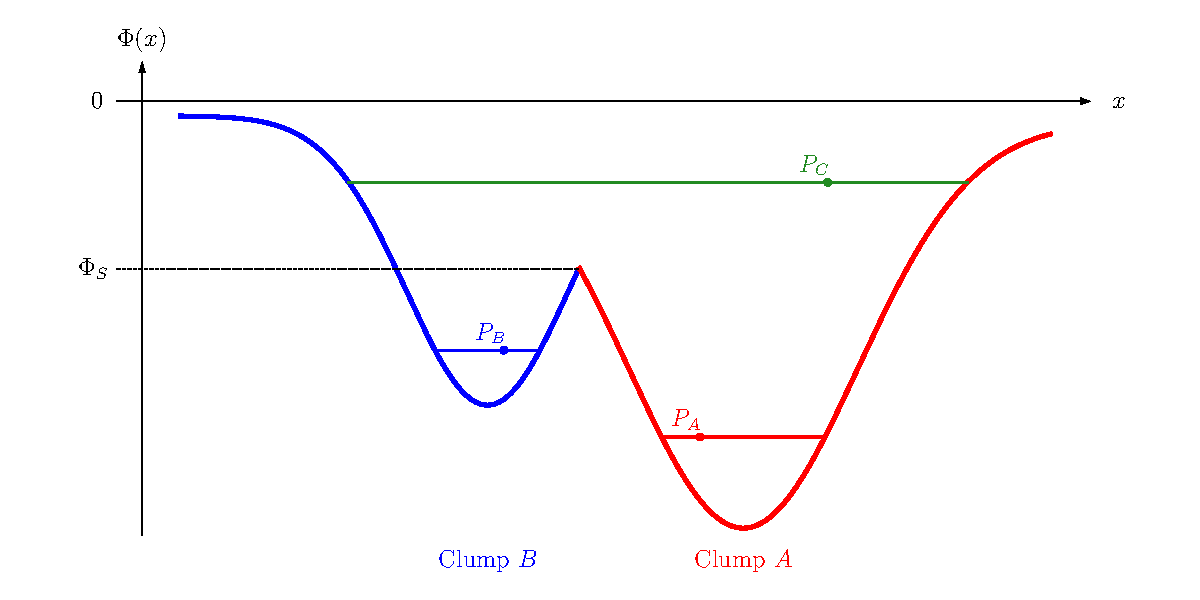
\includegraphics[width=.95\linewidth, keepaspectratio]{images/potentials_new.pdf}}%
  \caption{Simple sketch of the gravitational potential of a halo that
    consists of two clumps, $A$ and $B$.  The position of the
    horizontal lines marks the energies of three example particles,
    $P_A$, $P_B$, and $P_C$, while the length of the lines shows the
    spatial extent of the orbits.  We call particles like $P_A$ and
    $P_B$ ``strictly bound'', as their predicted orbit boundaries
    don't allow them to escape from the clump they are assigned to.
    Particle $P_C$ however, although energetically bound to clump $A$,
    can wander off deep into clump $B$, and for that reason is called
    ``loosely bound''. To discriminate between these two types of
    particles, we use the potential of the saddle point between clump
    $A$ and $B$ marked as $\Phi_S$.
  }%
  \label{fig:potentials}
  %	\endminipage\hspace*{\fill} 
\end{figure}
%
%Consider an isolated halo that consists of two clumps, $A$ and $B$, where $B$ is a smaller clump nested within clump $A$.
%Their potentials are qualitatively depicted in Figure \ref{fig:potentials}.
%The total energy per particle mass $E/m_p$ of the particle on the graph is the difference between the plotted norm of the potential and the kinetic energy on the $y$-axis.
%Because $v^2\geq 0$, the spatial boundaries of a particle's trajectory can be found by following the curve of allowed kinetic energies of the particle to the points where $v^2 = 0$.
%The marked particle $P$, even though initially assigned to clump $B$ and considered bound by condition \ref{eq:boundv}, is energetically allowed to leave the boundaries of clump $B$ and wander off deep into the neighbouring clump $A$.
%Should that occur in between two consecutive snapshots, then the particle $P$ will be rightfully found to belong to clump $A$ in the following snapshot.
%As such, the particle $P$ shouldn't be considered strictly bound to clump $B$.



%Three particles assigned to $B$ with different kinetic energies are marked, representing three different cases:
%%
%\begin{itemize}
%	\item Particle $\alpha$ has a kinetic energy higher than the potential, it is clearly not bound to the clump $B$.
%	\item Particle $\beta$ has a kinetic energy lower than the potential at that distance from the centre of mass, so it will remain bound on an elliptic trajectory around the centre of mass.
%	\item Particle $\gamma$ is considered energetically bound to the clump just like $\beta$, i.e. it satisfies condition \eqref{eq:boundv}, but it won't necessarily remain on an elliptic trajectory around clump $B$'s centre of mass: Because of clump $A$'s neighbouring potential, the particle can leave the boundaries of clump $B$ and wander off deep into clump $A$.
%\end{itemize}
%%

%To address this occurrence the condition for a particle to be bound needs to be modified appropriately: its trajectory must never reach the common surface between any two clumps.
%Defining $\Phi_S$ to be the potential of clump $B$ at the interface to any neighbouring structure that is closest to $B$'s centre of mass, the condition for a particle to be bound \emph{exclusively} to a particular clump can be written as
%
%\begin{equation}
%	v < \sqrt{ - 2(\Phi - \Phi_S) } \label{eq:boundv_corr}
%\end{equation}


%We have verified that according to expectations, demanding particles to be exclusively bound, i.e. satisfying condition \ref{eq:boundv_corr}, will tend to find more unbound particles than not doing so, where particles close to the centre of mass are be more likely to be exclusively bound than the particles closer to the outer boundary of the sub-halo.

When computing the velocity of the particle, it is important to use
the velocity {\it relative} to the velocity of the sub-halo centre of
mass (also called the bulk velocity of the sub-halo).  Because of this
requirement, the unbinding process has to be performed iteratively,
since removing a particle that is unbound requires to recompute the
centre of mass velocity.  Let us finally repeat that the particle
unbinding is performed recursively, following the sub-halo hierarchy
from the bottom up.  Starting with the lowest (finest) level of
sub-haloes, unbound particles are assigned to the higher (coarser)
level of parent sub-halo for unbinding, and so on following the
structure hierarchy.  Particles that are unbound from all sub-haloes
are collected into the main halo, marking the end of the hierarchical
unbinding process.



    %====================================================================
\section{Merger Trees: Basic Principles}\label{chap:my_code}
%====================================================================

In this work, we adopt the terminology set by the ``Sussing Merger
Tree Comparison Project'' \citep{SUSSING_COMPARISON,
  SUSSING_CONVERGENCE, SUSSING_HALOFINDER,leeSussingMergerTrees2014a}.
For sake of clarity, we repeat here some important definitions:

\begin{itemize}
  
\item For two snapshots at different times, a halo from the first one
  (i.e. higher redshift) is always referred to using the capital
  letter $A$ and a halo from the second one (i.e. lower redshift)
  using $B$.
  
\item Recursively, $A$ itself and progenitors of $A$ are all
  \emph{progenitors} of $B$.  When it is necessary to distinguish $A$
  from earlier progenitors, the term \emph{direct progenitor} will be
  used.
  
\item Recursively, $B$ itself and descendants of $B$ are all
  \emph{descendants} of $A$.  When it is necessary to distinguish $B$
  from later descendants, the term \emph{direct descendant} will be
  used.
  
\item In this work, we restrict ourselves to merger trees for which
  there is \emph{precisely one direct descendant for every halo}.
  
\item When there are multiple direct progenitors, it is required that
  one of these is identified as the \emph{main progenitor}.
  
\item The \emph{main branch} of a halo is a complete list of main
  progenitors tracing back along its cosmic history.
  
\end{itemize}
We finally define an important convention we use here: when no
distinction between sub-haloes and main haloes is necessary, they are
collectively referred to as \emph{clumps}.

\subsection{Linking Clumps Across Snapshots}

The aim of a merger tree code is to link haloes from an earlier
snapshot to haloes in the consecutive snapshot, i.e. to find all the
descendants of the haloes in the earlier snapshot. If we do this 
successfully each snapshot, then we can follow the formation history of 
haloes throughout the simulation. In particular, this will enable us
to track the mass growth of haloes as well as the merging of different
sub-haloes during the course of the simulation. 
To illustrate the idea, a merger tree of a main halo generated by 
\texttt{ACACIA} during a simulation is shown in Figure~\ref{fig:mergertree}.
In this particular case, we were able to track the formation history of the 
main halo down to redshifts $z > 3$. By linking progenitors and descendants 
throughout the simulation many branches of the tree are revealed. 
Each branch represents a clump that eventually merged into the main halo 
which we chose as the root of the tree at redshift zero.

Merger events occur when a clump, identified as such in a previous
snapshot, disappears from the list of clumps in the next snapshot. In
the case of a halo, it usually first becomes the sub-halo of another
halo and can be followed as such in many subsequent snapshots. After
some time, this sub-halo can merge into another sub-halo or dissolve
completely due to numerical over-merging. In both cases, the sub-halo
disappears completely from the clump catalogue.

\begin{figure}
  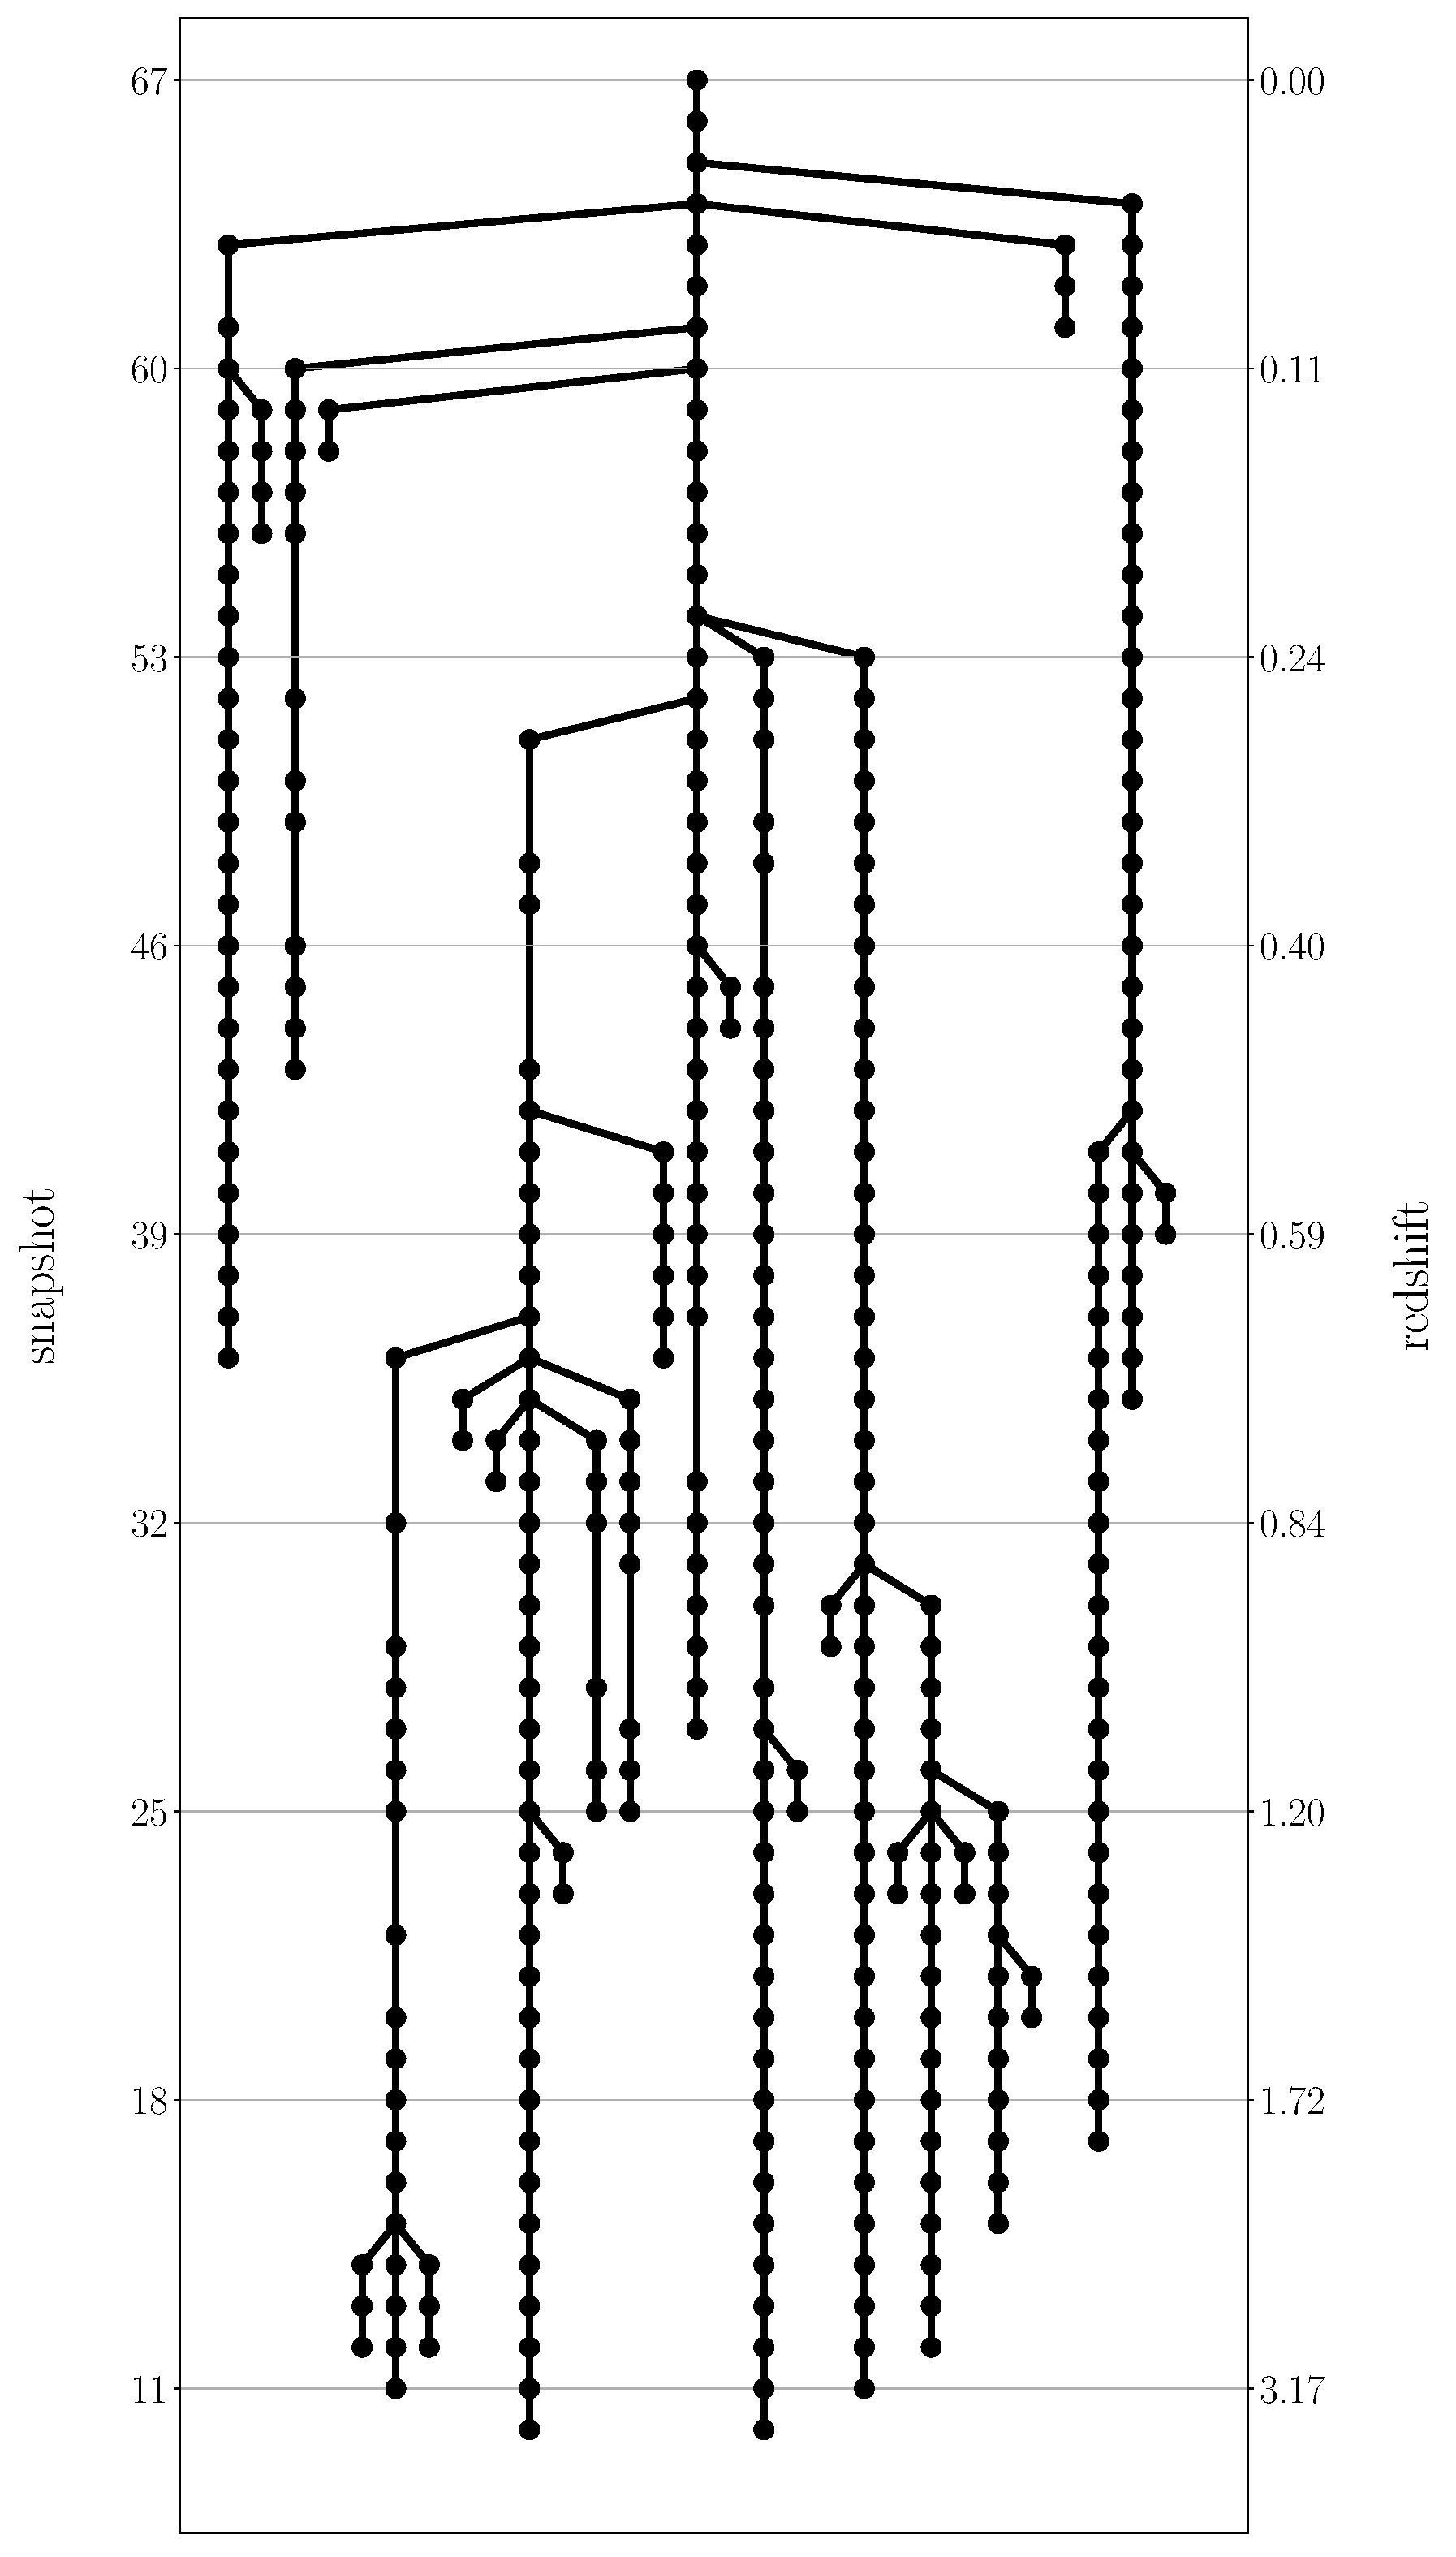
\includegraphics[width=\linewidth]{images/merger_tree_example.pdf}%
  \caption{The merger tree of a main halo at redshift zero as found by
    \texttt{ACACIA}.  This tree was extracted from a low resolution
    cosmological DMO simulation containing $64^3$ particles for
    illustrative purposes. Using higher resolutions quickly leads to
    hundreds and thousands of branches, resulting in a rather messy
    plot. On the $y$ axis, the snapshot numbers and their
    corresponding redshifts are given.  The $x$ axis has no physical
    meaning.  Each dot represents a clump identified at the given
    snapshot.  Two dots connected by a vertical line represent clumps
    that have been linked as main progenitor and main descendant.
    Diagonal lines depict merging events. In this tree, a few links
    between two dots are larger than others.  These are cases where
    clumps merge temporarily, but then re-emerge later as separate
    clumps (see the example shown in Figure~\ref{fig:jumper-demo}).
    We discuss these cases and how they are dealt with in
    Section~\ref{sect:jumpers}. }
  \label{fig:mergertree}
\end{figure} 

A straightforward method to link progenitors with descendants in two
consecutive snapshots is to trace individual particles using their
unique particle ID. All merger tree codes use this simple technique
\citep[][]{ConsistentTrees, LHaloTree, D_Trees,
  knebeImpactBaryonicPhysics2010, tweedBuildingMergerTrees2009,
  elahiPeaksMaxwellianSea2011, jungEffectsLargescaleEnvironment2014,
  rodriguez-gomezMergerRateGalaxies2015} with the notable exception of
the code \texttt{JMERGE} described and tested in
\cite{SUSSING_COMPARISON}.

Linking a progenitor to a descendant means checking how many particles
of the progenitor halo or sub-halo end up in the descendant halo or
sub-halo.  Naturally, these tracer particles may end up in multiple
clumps, giving multiple descendant candidates for a progenitor.  In
such cases, the most promising descendant candidate will be called the
\emph{main descendant}.  To find a main progenitor and a main
descendant, a merit function $\mathcal{M}$ has to be defined, which is
to be maximised or minimised, depending on its definition.  An
overview of the merit functions that are used in other merger tree
algorithms is given in Table~1 of \cite{SUSSING_COMPARISON}.  The
merit function used in our implementation is given in
Equation~\ref{eq:merit}.

Sometimes, unfortunately, linking progenitors to descendants is not as
straightforward as described so far. We now discuss two circumstances
where special care must be taken to define robust links between
different snapshots: fragmentation events and temporary merger events.

%Because galaxies form inside the potential well dark matter haloes,
%knowledge of how many merging events a halo underwent during its
%lifetime is crucial for accurate mock galaxy catalogues.  After a
%merging event, the galaxy of the smaller halo that has been
%``swallowed up'' by a bigger one has no reason to simply vanish
%without a trace.  The ``swallowed up'' halo might become a sub-halo,
%or, if it is small enough or after some time, it might not be
%detectable as substructure in the simulation any more.  Galaxies of
%haloes that dissolve in this manner are referred to as ``\emph{orphan
%galaxies}'' \citep[e.g.][]{subfind}.

\begin{figure}
  \centering
  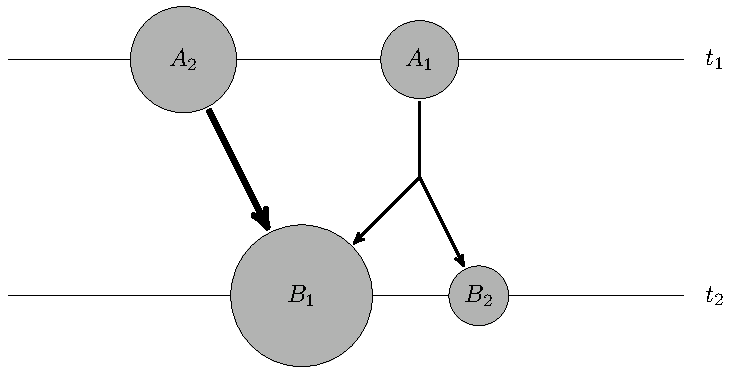
\includegraphics[width=.9\linewidth]{./images/tikz/fracture.pdf}
  \caption{Illustration of a progenitor $A_1$ at time $t_1$ which is
    partially merged into a descendant $B_1$ at time $t_2 > t_1$, but
    some other part $B_2$ isn't.  Because $A_1$ is not the main
    progenitor of $B_1$, by assigning its descendant only according to
    the merit function \eqref{eq:merit} would not pass on its
    formation history to $B_2$, but treat it as newly formed.  The
    size of the circles represents the haloes' masses, the $x$-axis
    has no physical meaning.  }
  \label{fig:fracture}
\end{figure}

\subsection{Fragmentation Events}
\label{sect:frag}

%See https://arxiv.org/pdf/2010.03567.pdf Fig. 34
In our current approach, each progenitor can have only one
descendant\footnote{Note that \cite{springelSimulatingCosmicStructure2020a}
proposed another approach that allows explicitly fragmentation
events to be included in the merger tree analysis.}. We therefore need
to pick only one descendant within a possibly large ranked list of
descendant candidates, that all contain particles coming from the
progenitor.

Normally, this choice is performed according to the ranking provided
by the merit function, where the main descendant is ranked number 1.
Problems arise for example when the progenitor $A_1$ is not the main
progenitor of its main descendant $B_1$, but also has fragmented into
another viable descendant candidate $B_2$.  This situation is
schematically shown in Figure~\ref{fig:fracture}.

Relying only on the merit function \eqref{eq:merit}, progenitor $A_1$
will seem to have merged with $A_2$, the direct progenitor of $B_1$,
in order to form $B_1$.  The other fragment, $B_2$, will be treated as
a newly formed clump and the entire formation history of $B_2$ would
be lost. In order to preserve this history, we choose to prioritize the 
link from $A_1$ to $B_2$ over of merging progenitor $A_1$ into $B_1$.


It is simpler to deal with this case directly in the algorithm
than via the merit function. The resulting logic can be summarized as
follows: If $A_1$ is not the main progenitor of its main descendant
$B_2$, then we don't merge it into $B_2$ but we link it instead with
the first secondary descendants that considers $A_1$ as its
main progenitor.

%This way, we give priority to $A_1$ for being a progenitor to some descendant which is
%not its main descendant over merging it into its main descendant.  In
%other words: being a main progenitor will have more weight on the tree
%building scheme than being a main descendant.

\subsection{Temporary Merger Events}
\label{sect:jumpers}

\begin{figure}[!htbp]
    {
%        \renewcommand{\arraystretch}{0.1}
        \setlength\tabcolsep{0em}
    	\centering	
    	\begin{tabular}{|p{5.3cm}p{5.3cm}p{5.3cm}|}
    		\hline
    		%		 
    		{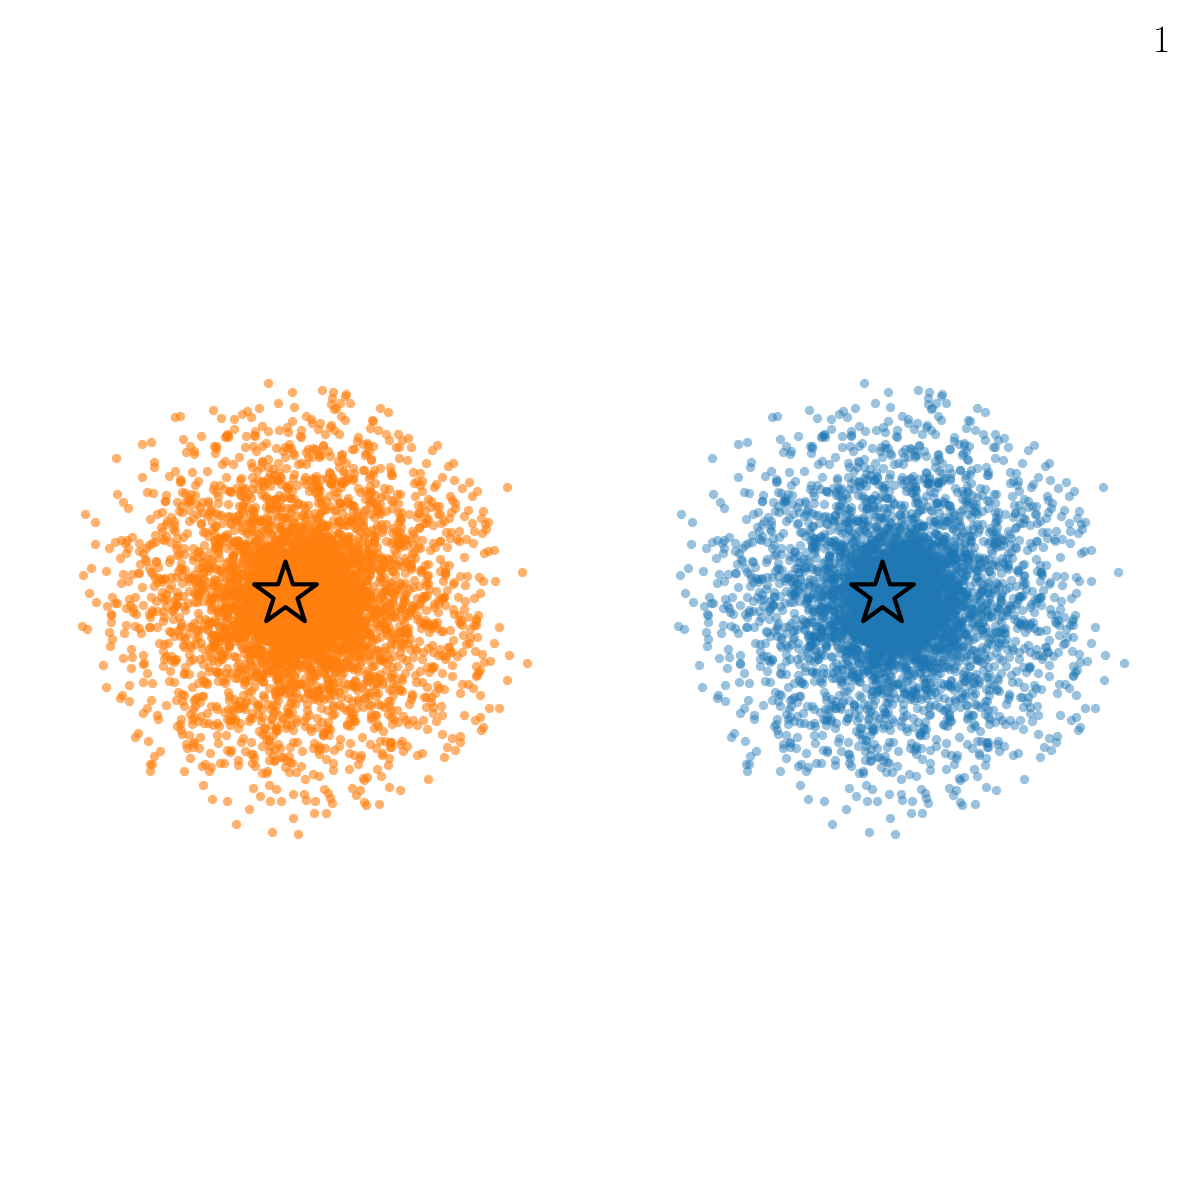
\includegraphics[width = 5.3cm]{images/jumper-demo/particleplot_00001.png}}	& 
    		{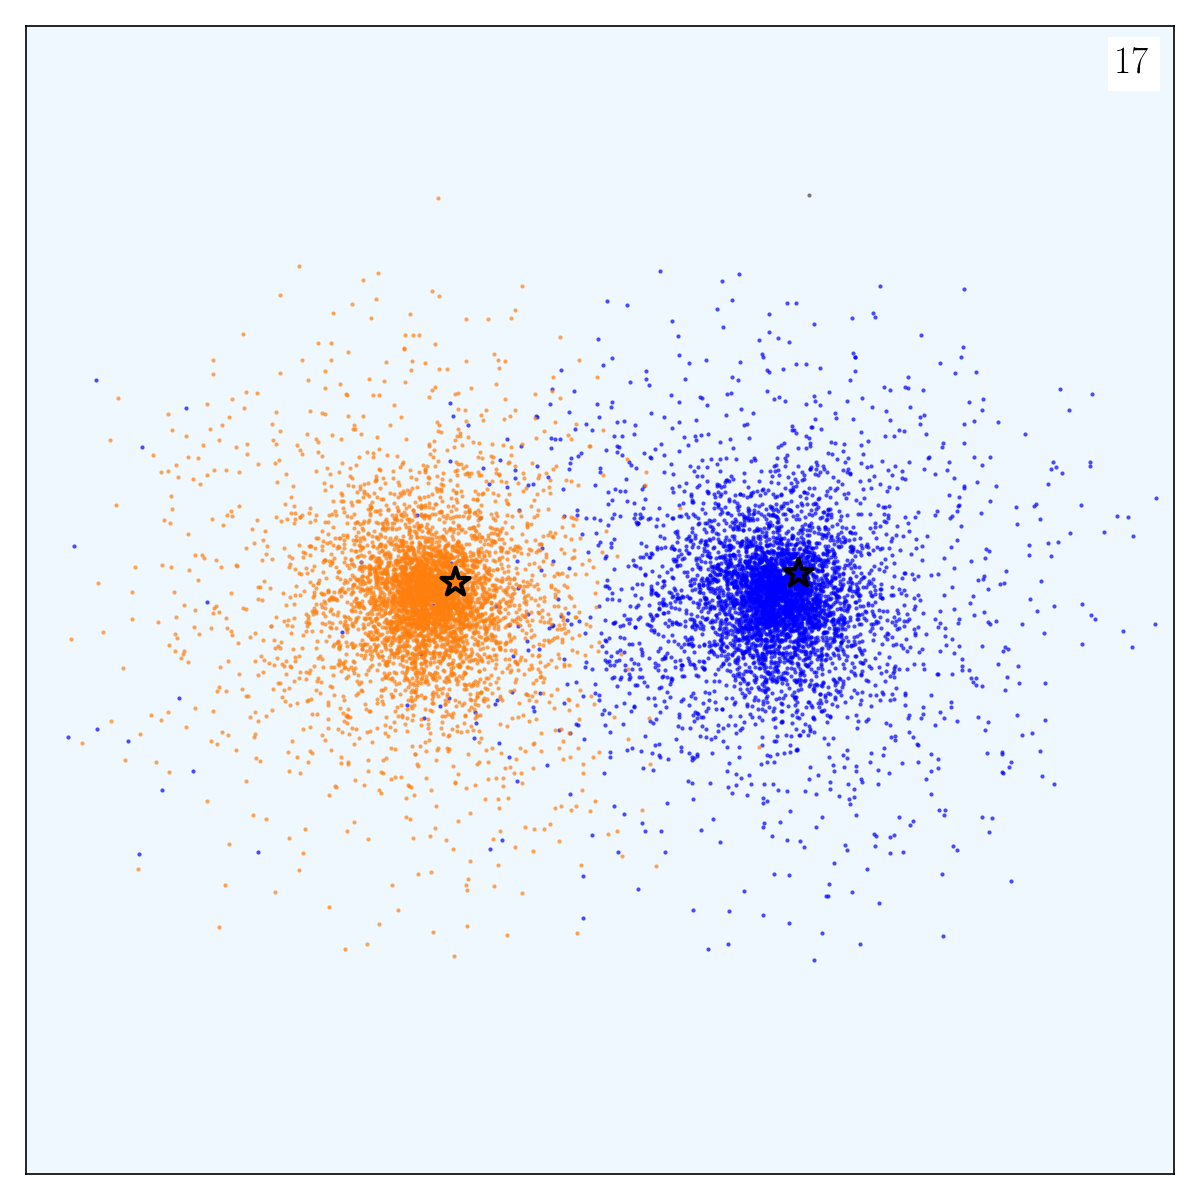
\includegraphics[width = 5.3cm]{images/jumper-demo/particleplot_00017.png}}	& 
    		{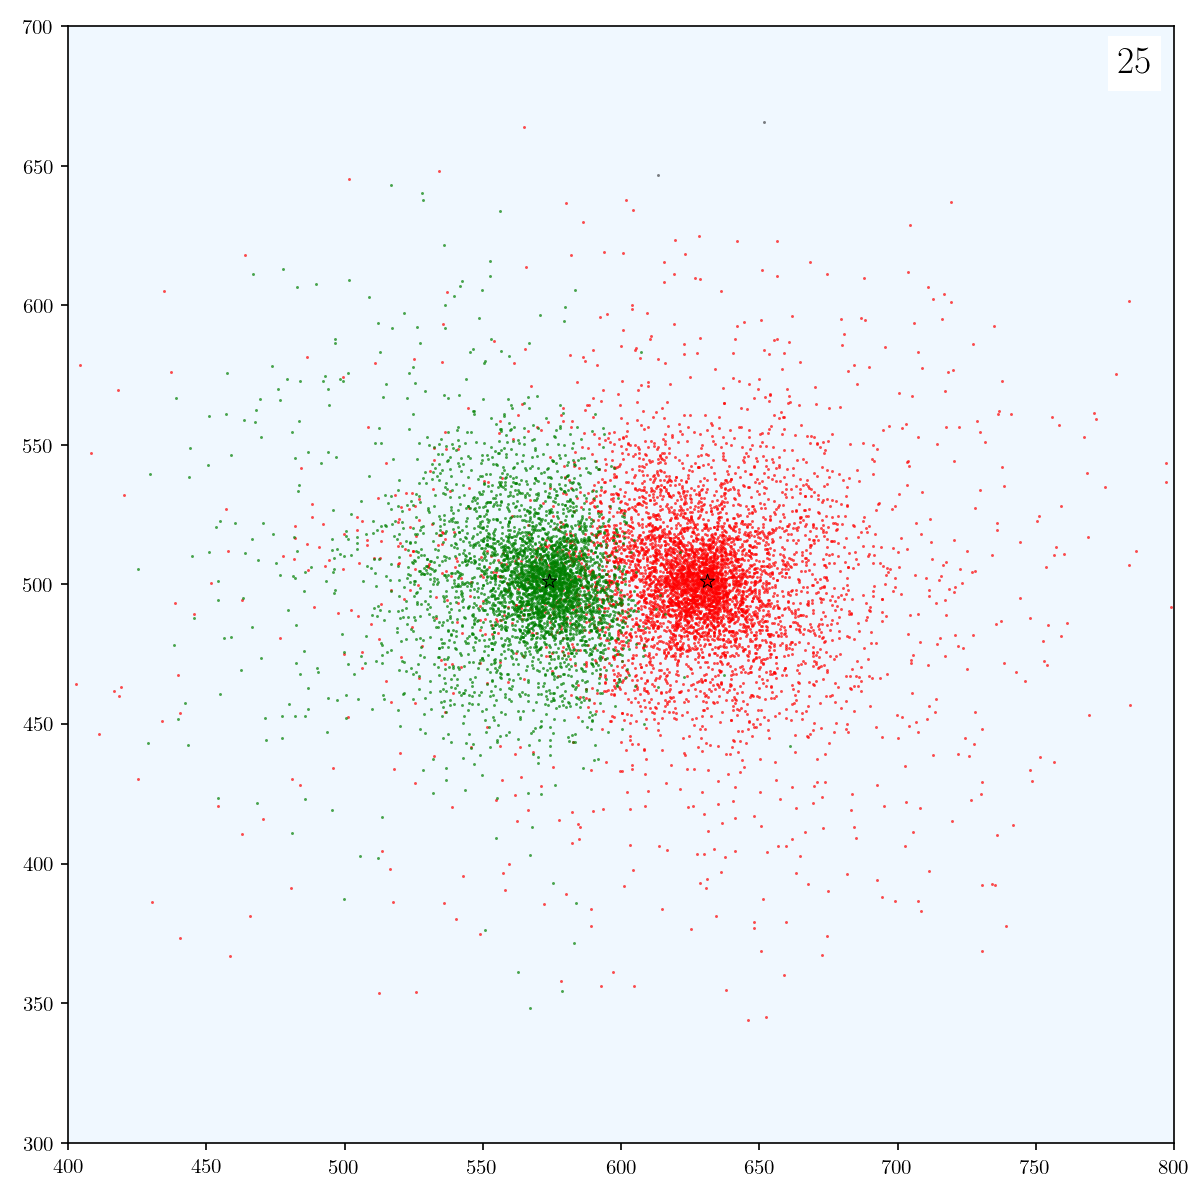
\includegraphics[width = 5.3cm]{images/jumper-demo/particleplot_00025.png}}  \\[-0.5em]
    		%
    		%
    		{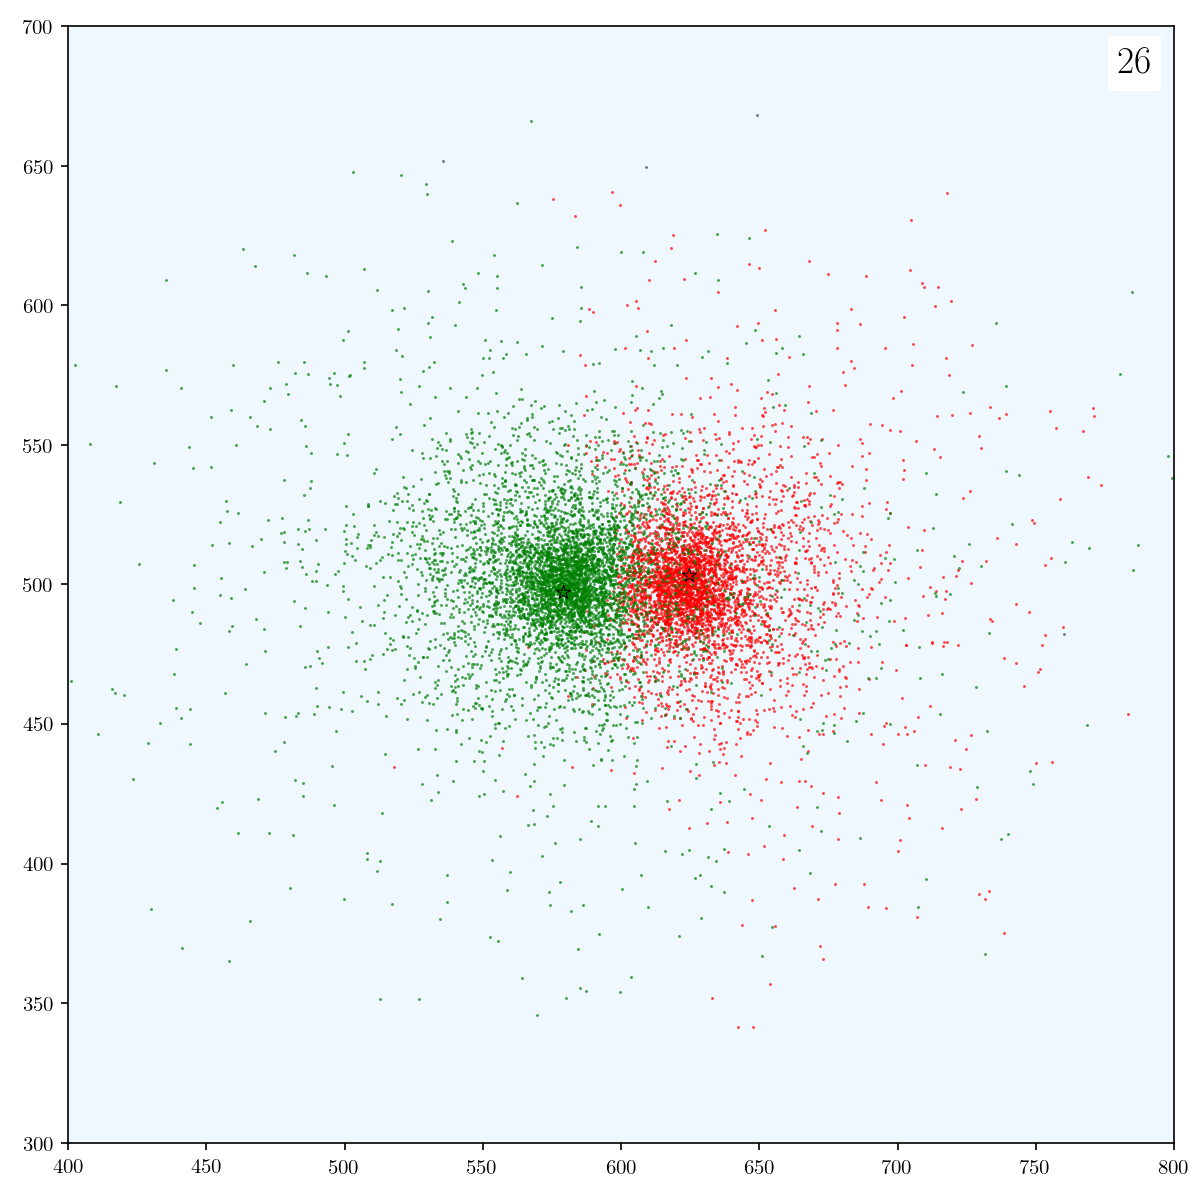
\includegraphics[width = 5.3cm]{images/jumper-demo/particleplot_00026.png}}	& 
    		{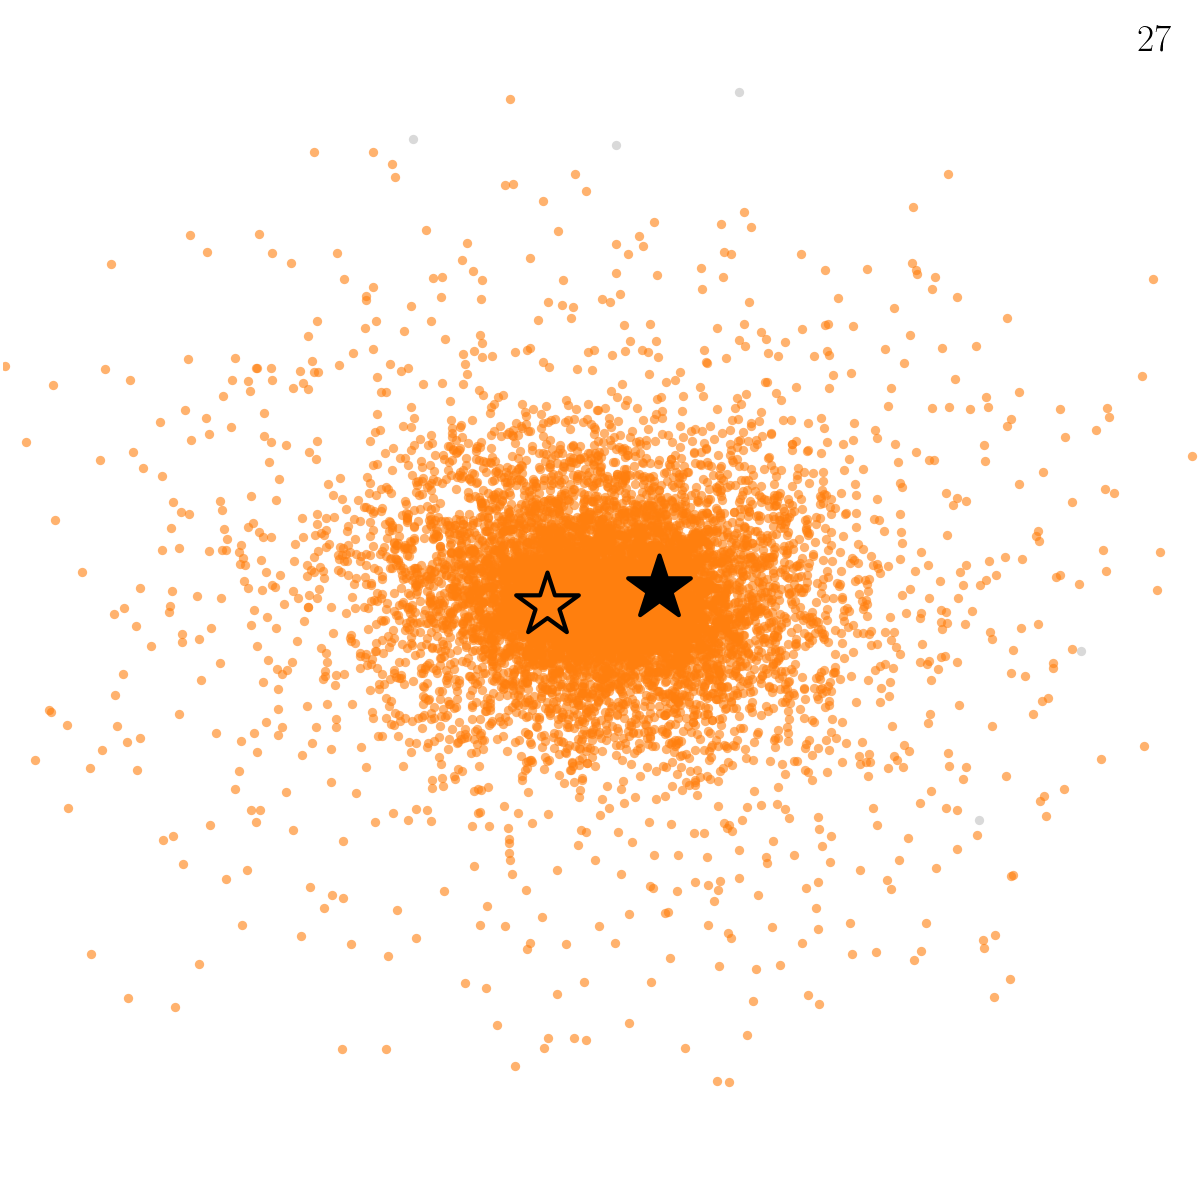
\includegraphics[width = 5.3cm]{images/jumper-demo/particleplot_00027.png}}	& 
            {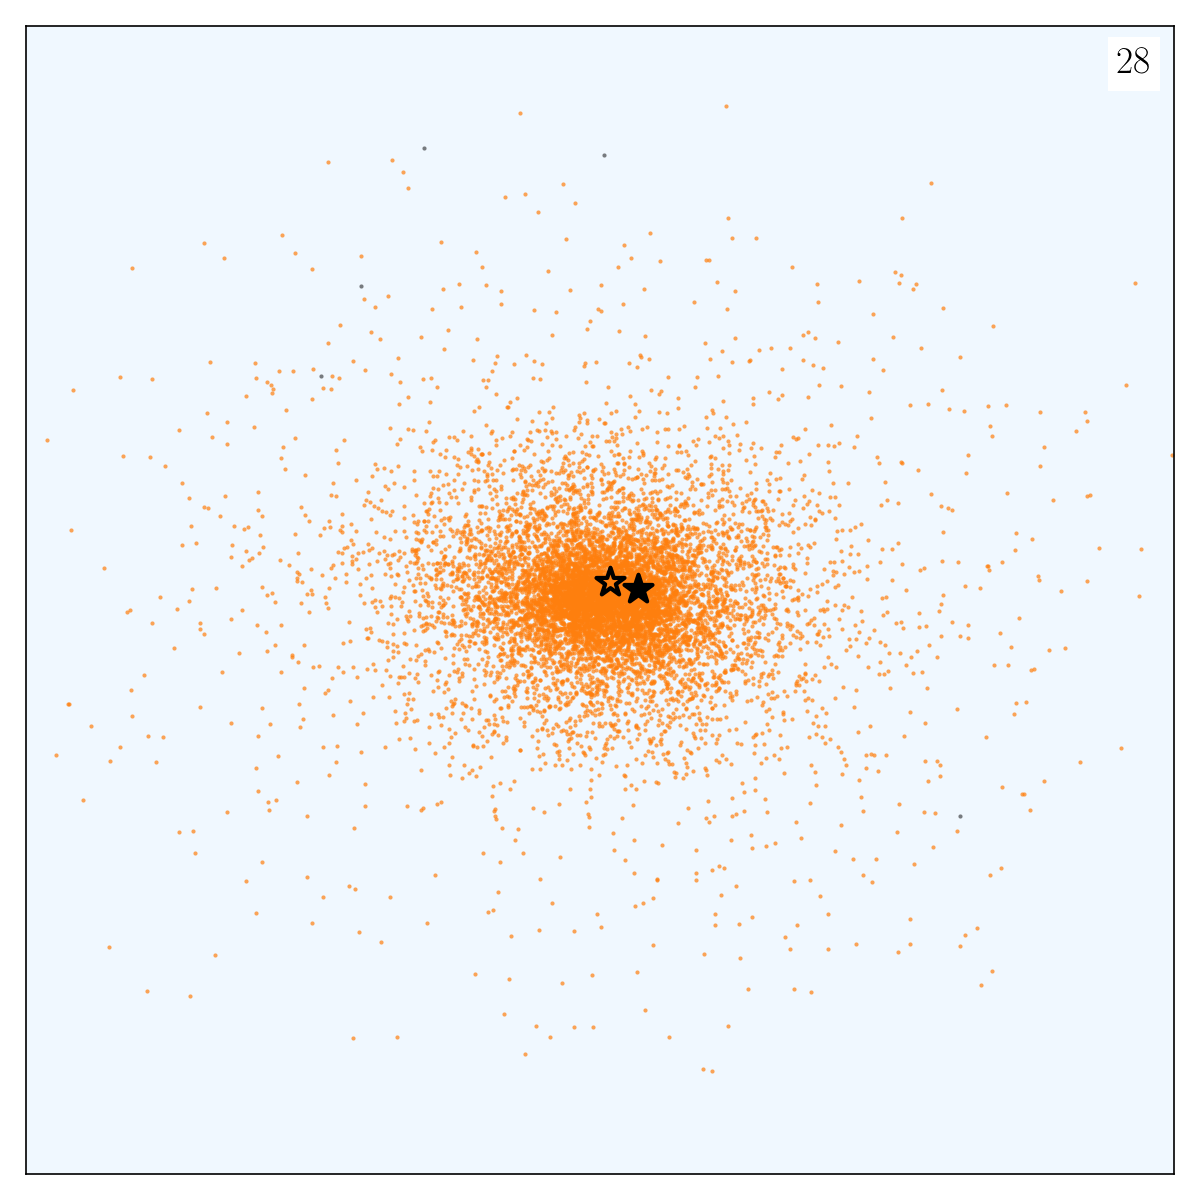
\includegraphics[width = 5.3cm]{images/jumper-demo/particleplot_00028.png}}	\\[-0.5em] 
    		%
            %
            {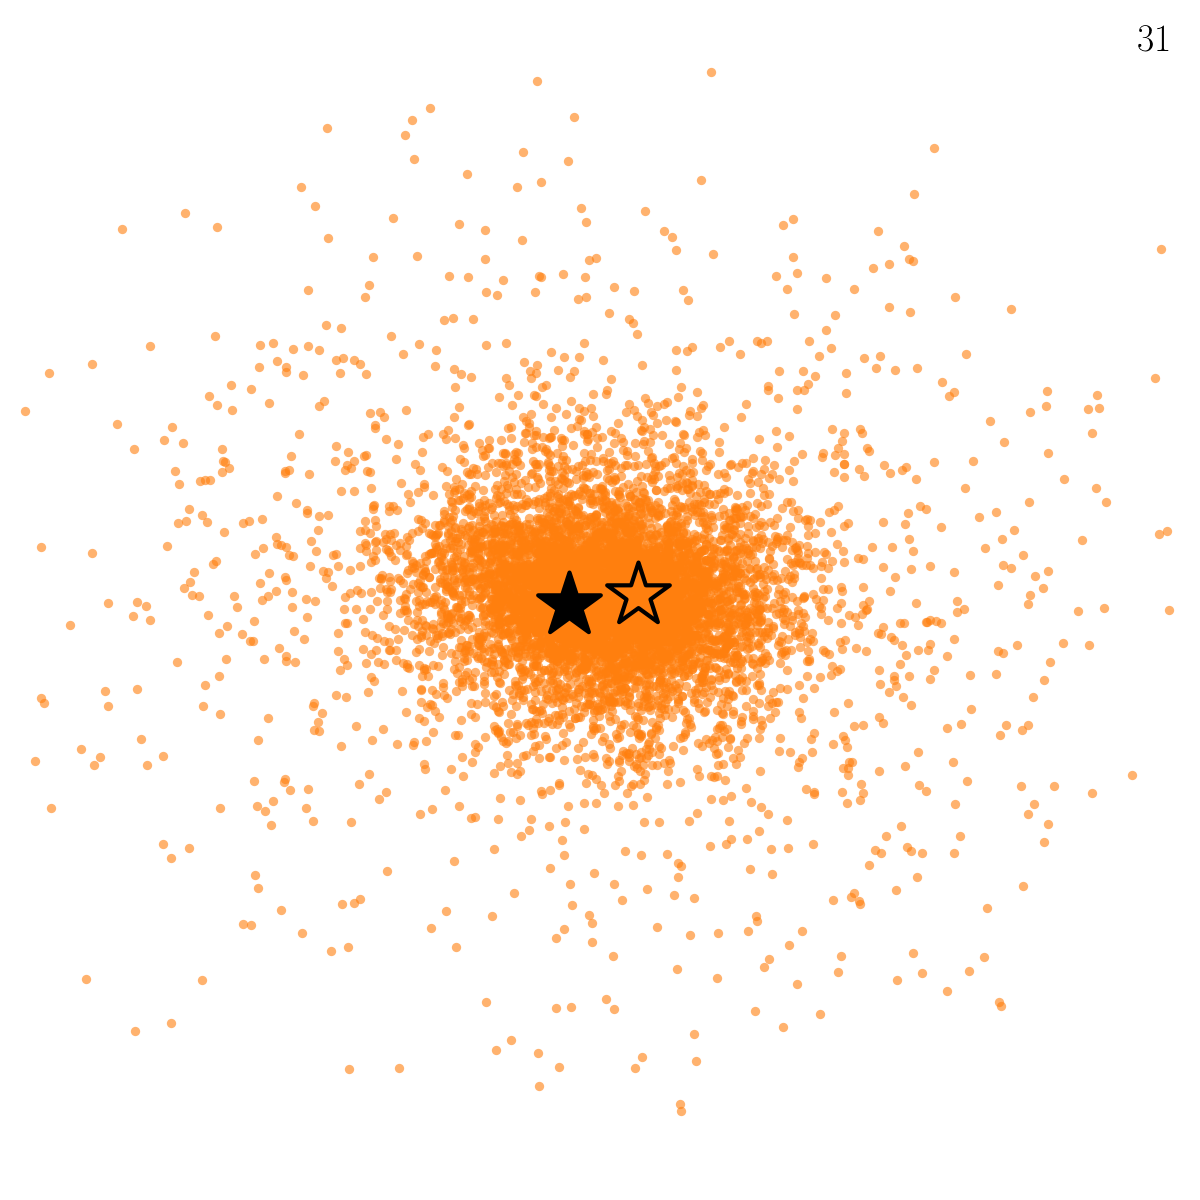
\includegraphics[width = 5.3cm]{images/jumper-demo/particleplot_00031.png}}    &
            {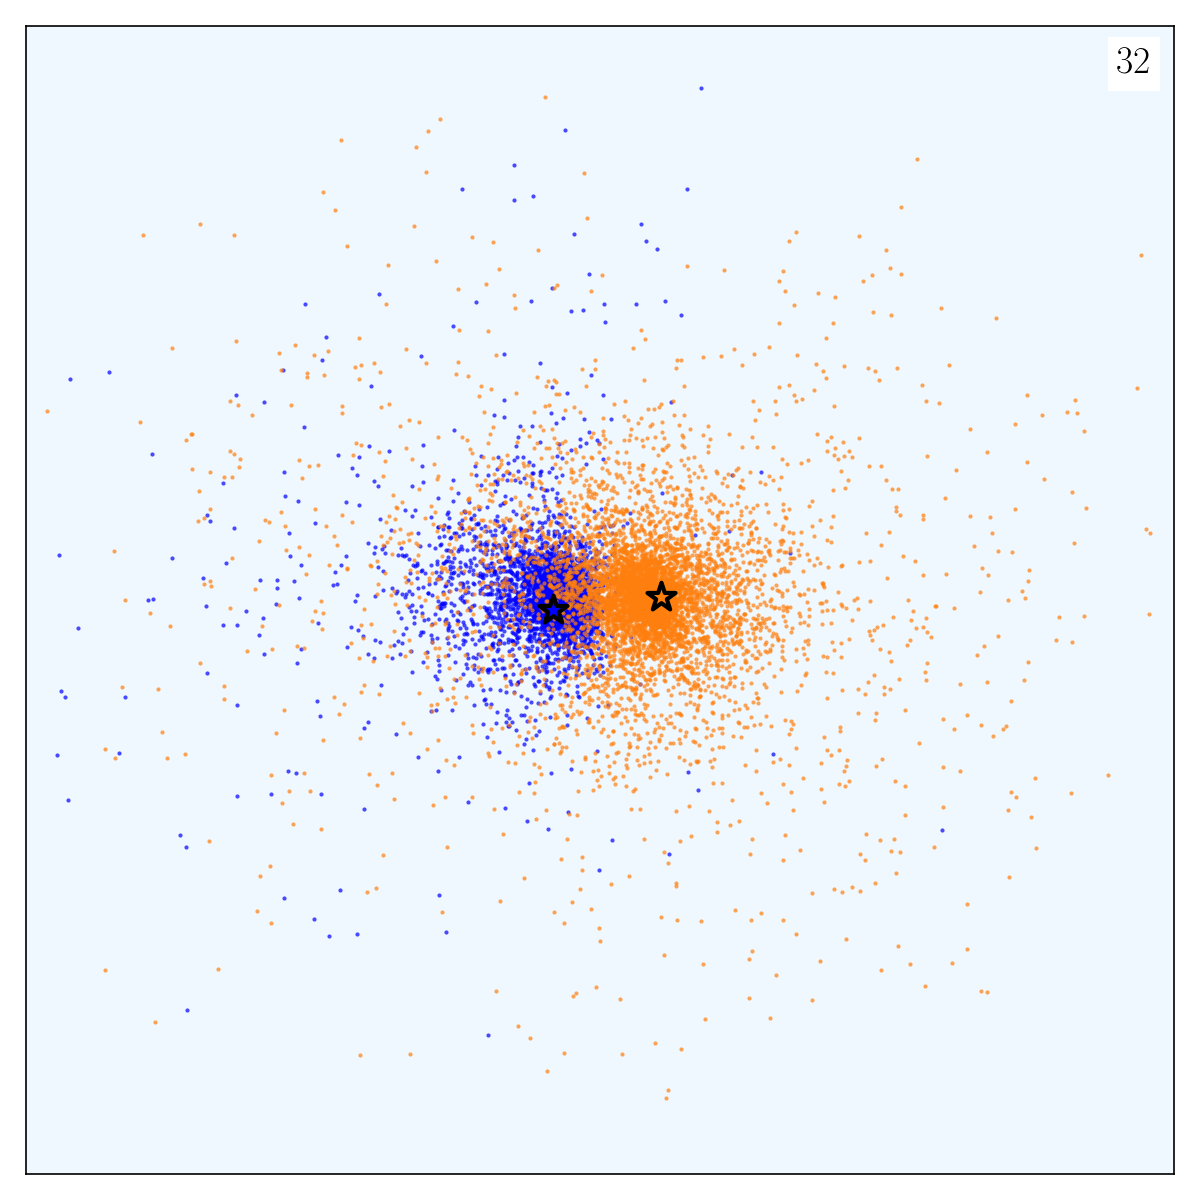
\includegraphics[width = 5.3cm]{images/jumper-demo/particleplot_00032.png}} 	&
            {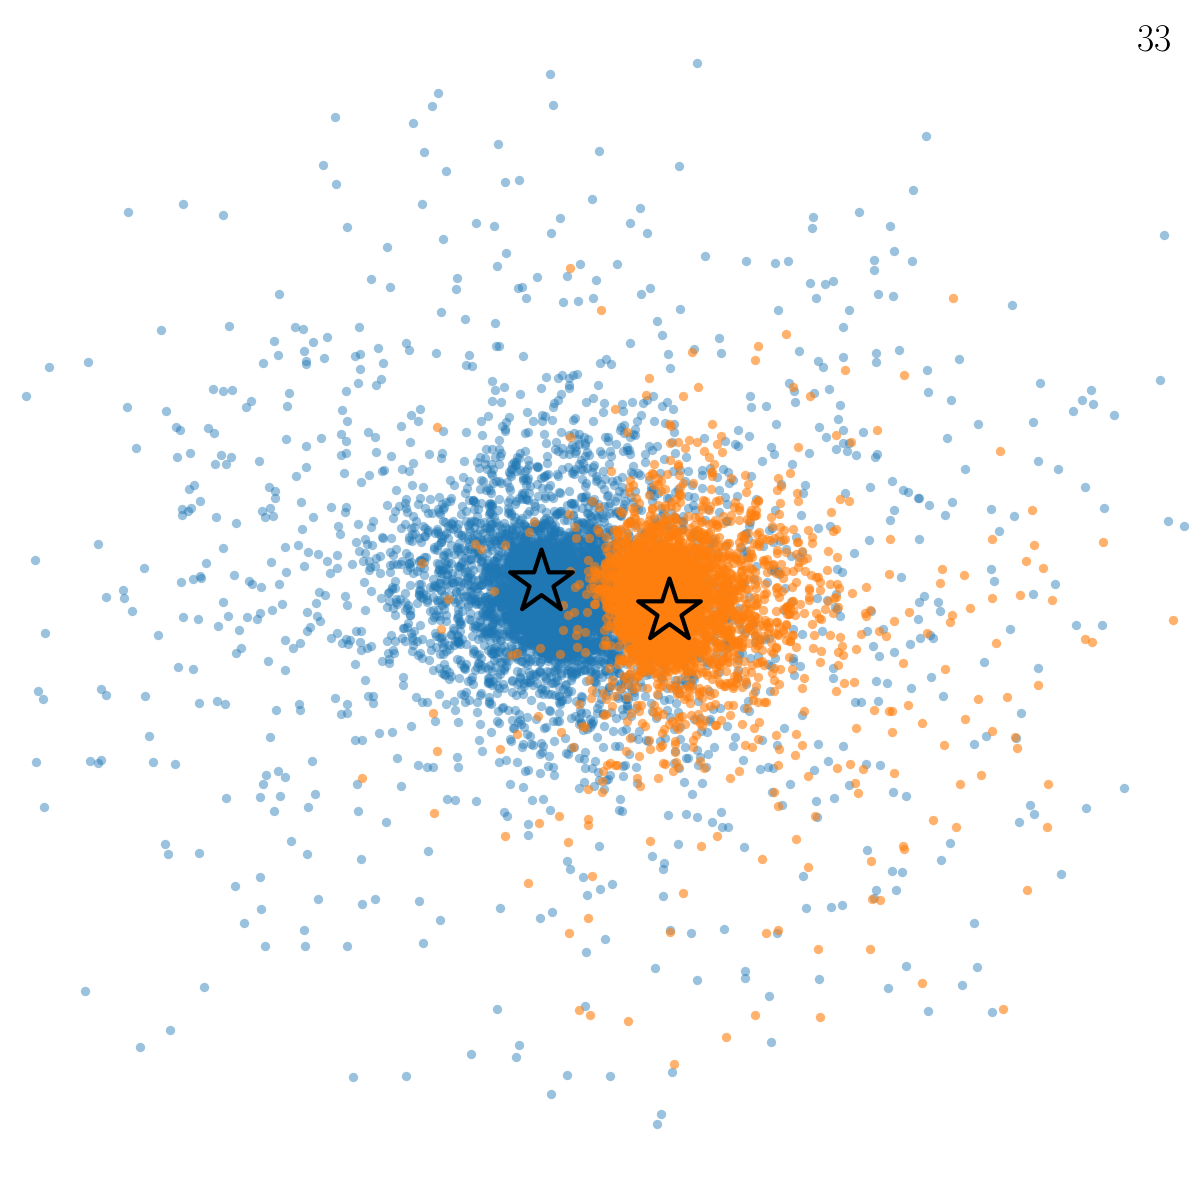
\includegraphics[width = 5.3cm]{images/jumper-demo/particleplot_00033.png}} 	\\[-0.5em]
    		%
            %
            {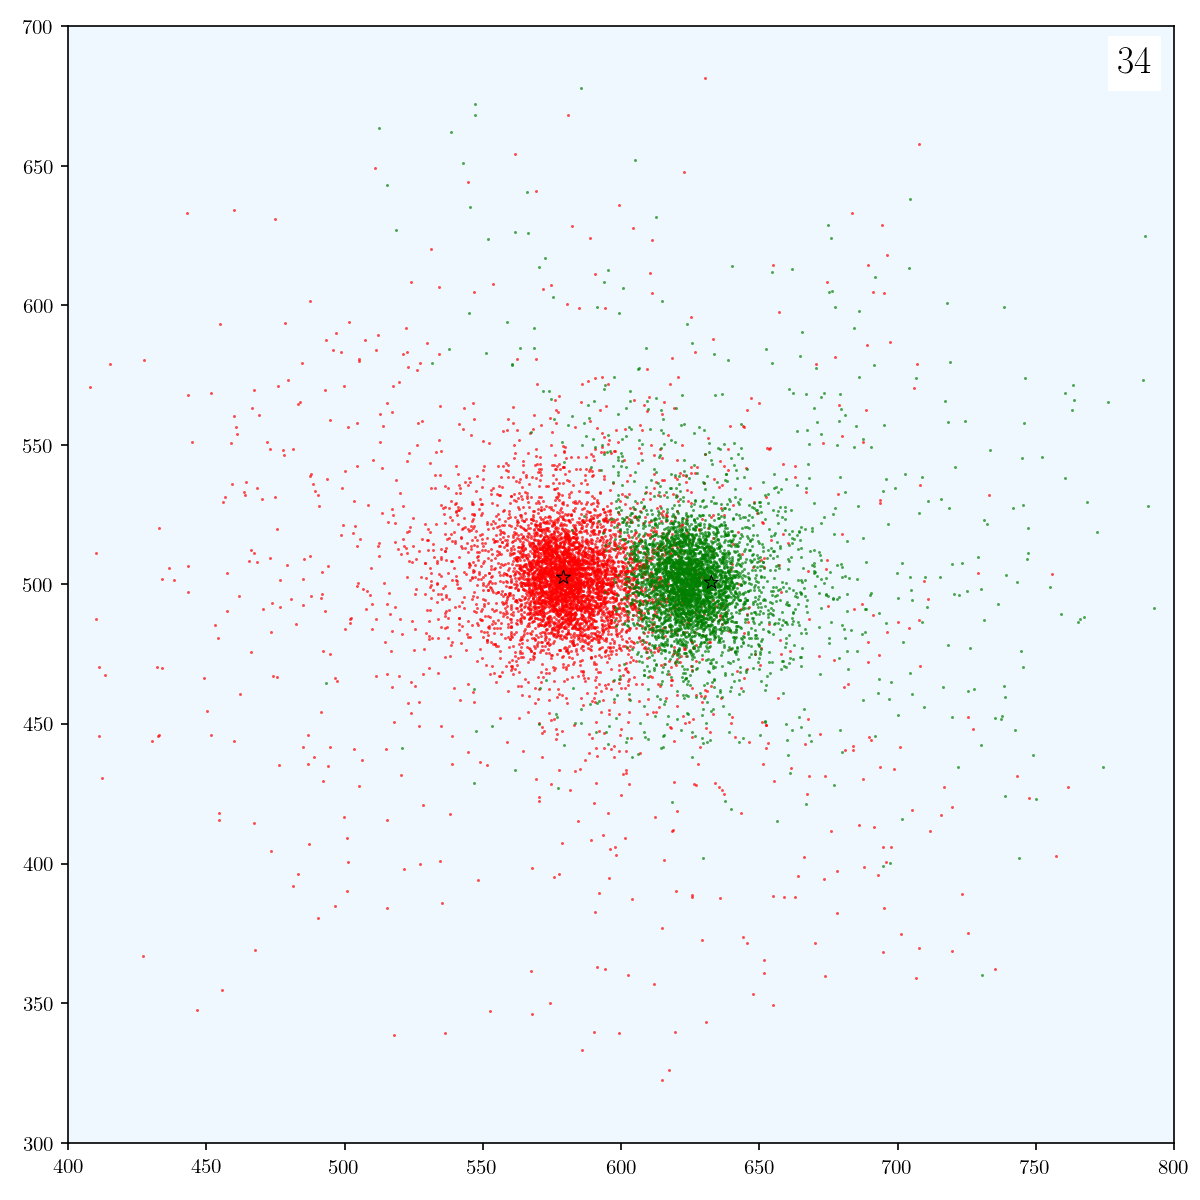
\includegraphics[width = 5.3cm]{images/jumper-demo/particleplot_00034.png}} 	& 
    		{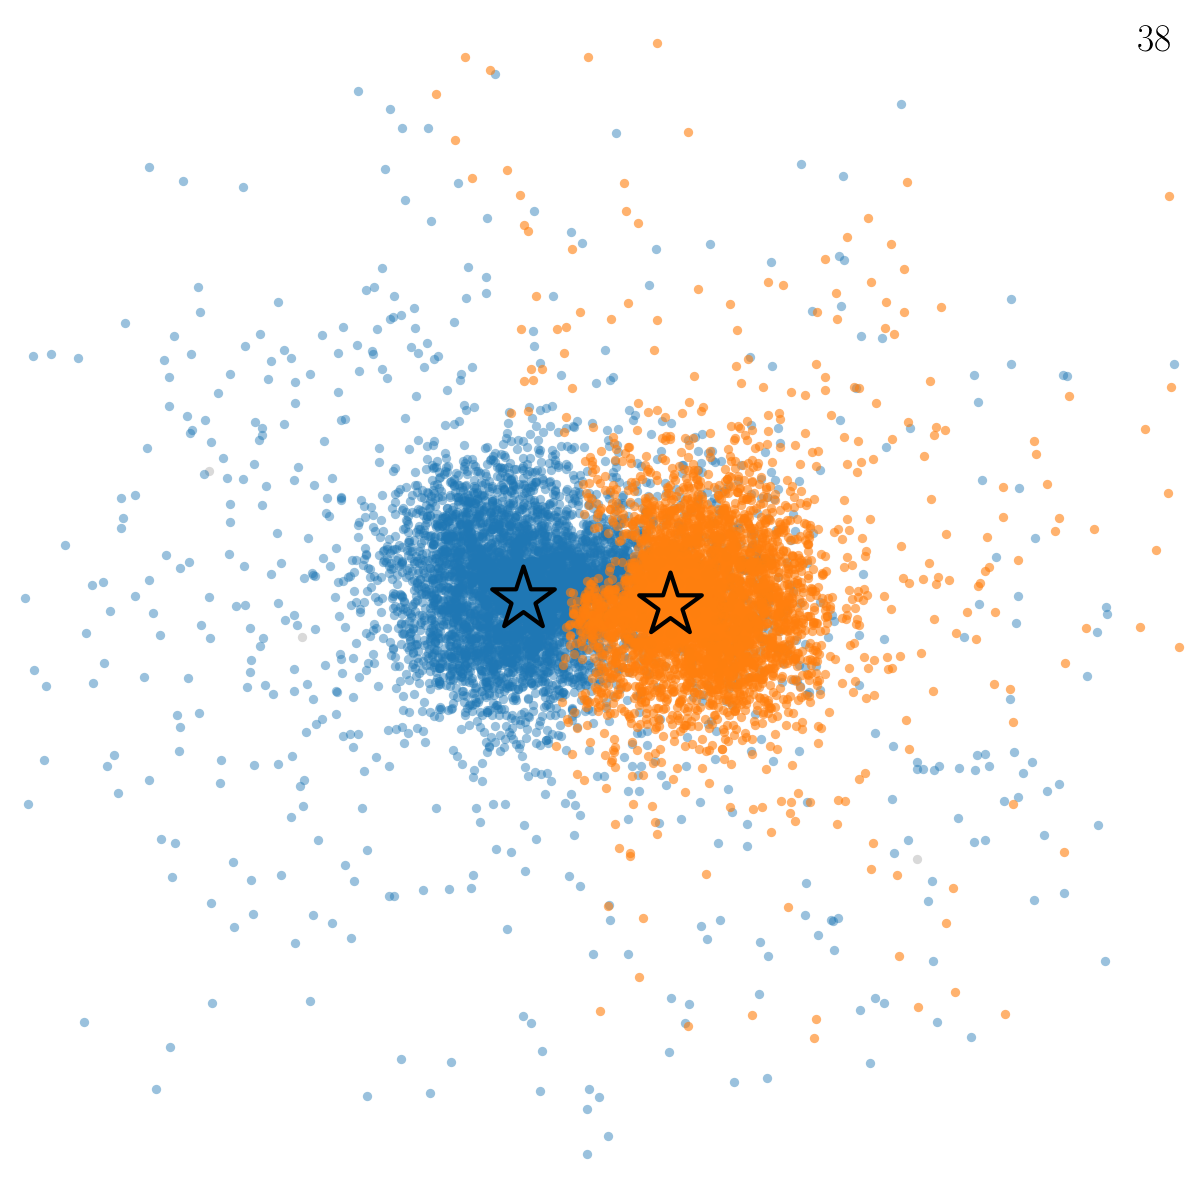
\includegraphics[width = 5.3cm]{images/jumper-demo/particleplot_00038.png}}	& 
            {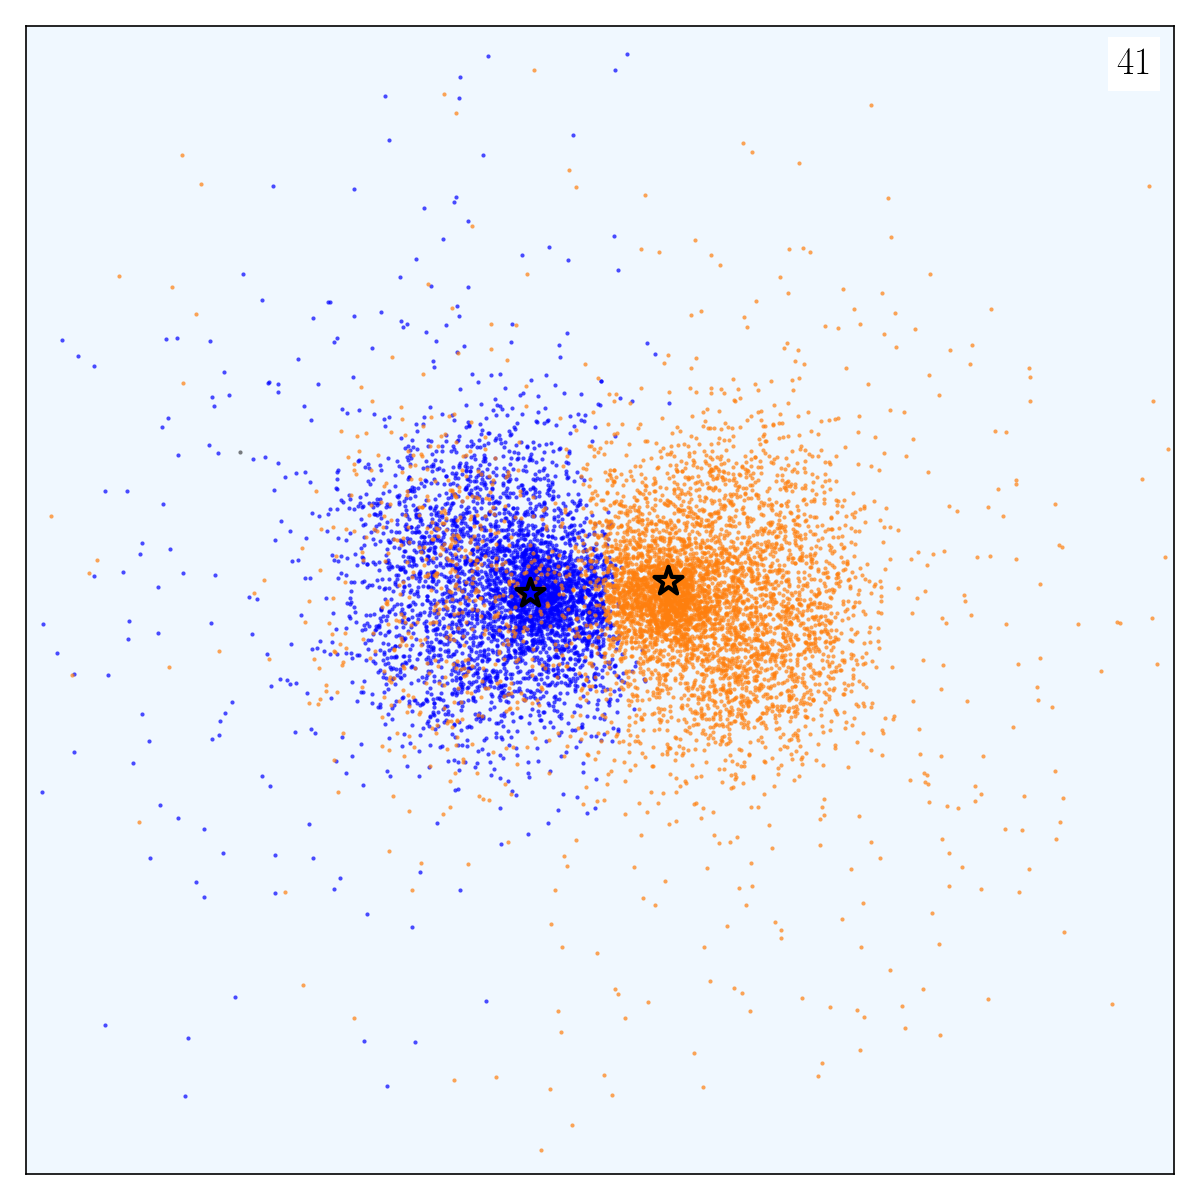
\includegraphics[width = 5.3cm]{images/jumper-demo/particleplot_00041.png}} 	\\%[-0.5em]
    		%
            %
%            {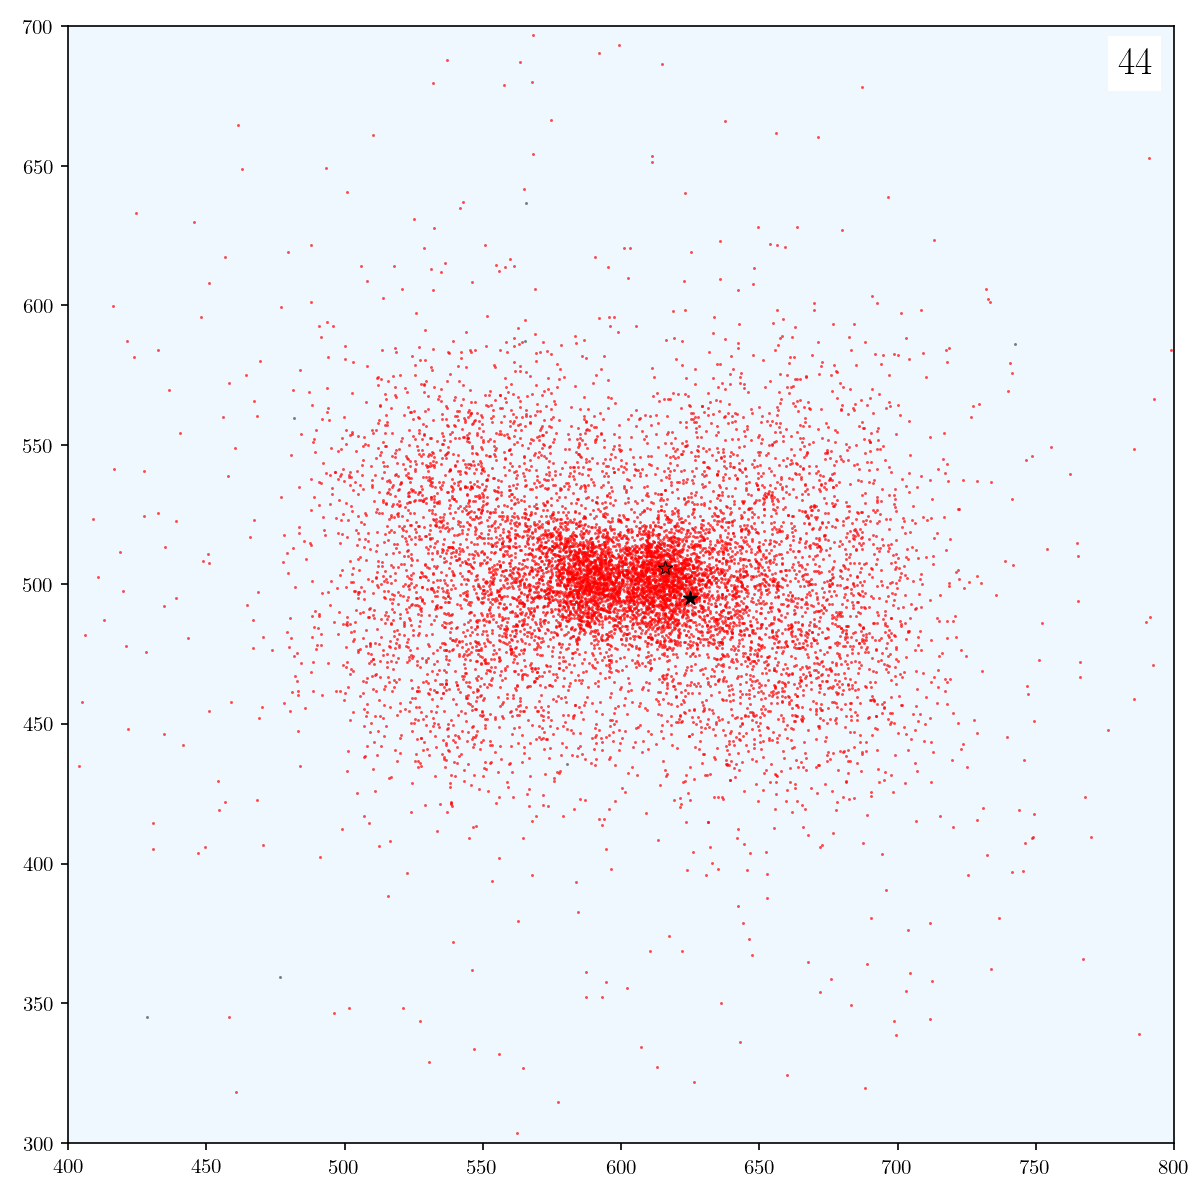
\includegraphics[width = 5.3cm]{images/jumper-demo/particleplot_00044.png}} 	& 
%    		{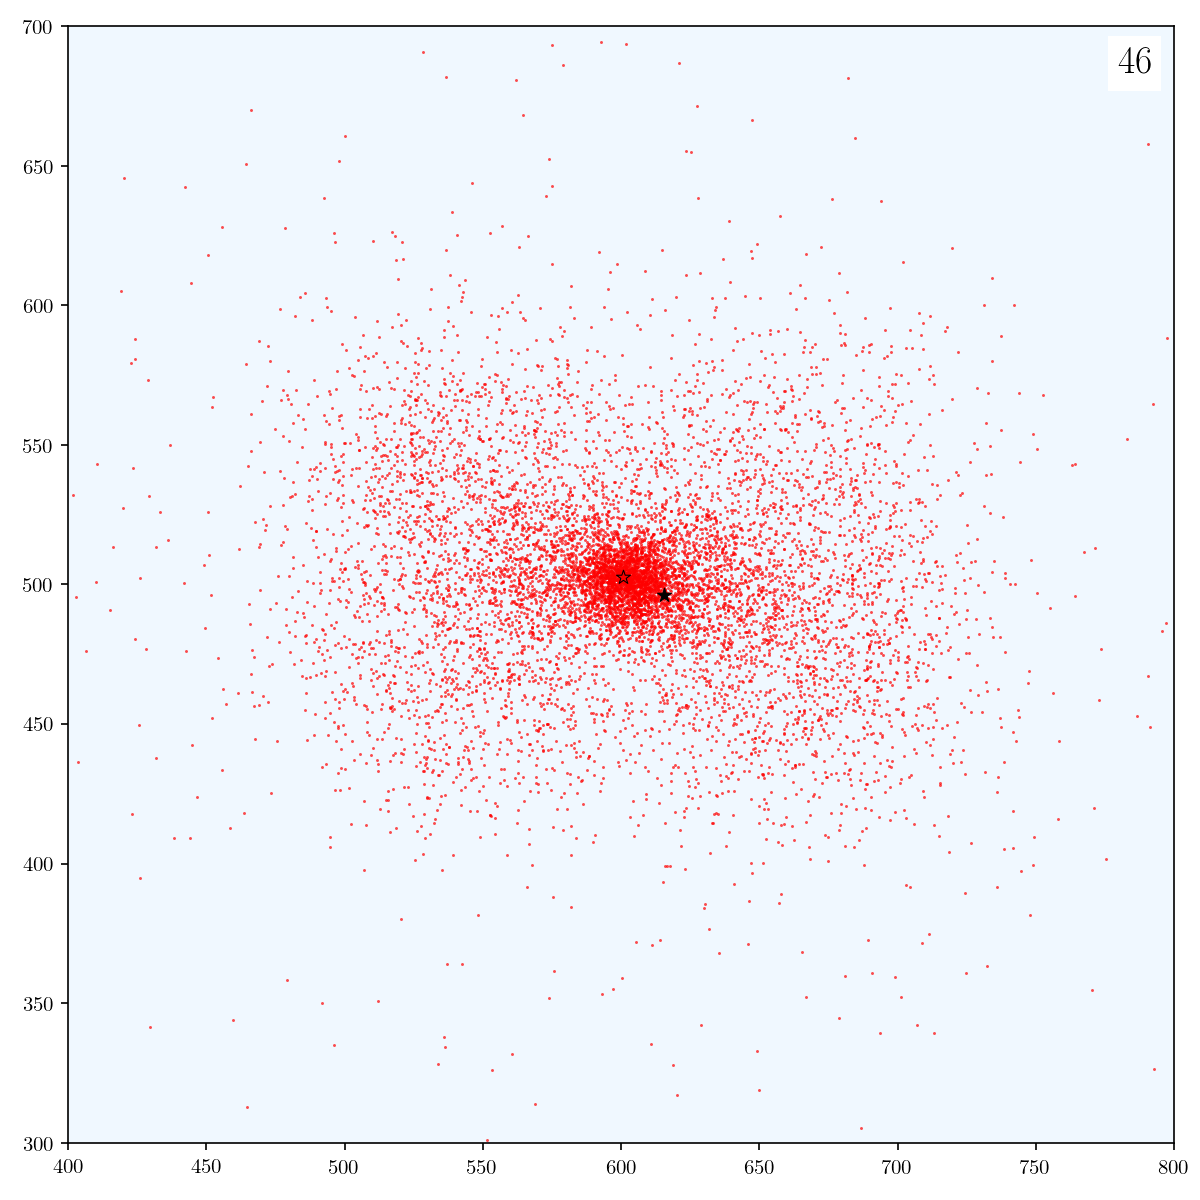
\includegraphics[width = 5.3cm]{images/jumper-demo/particleplot_00046.png}}	& 
%            {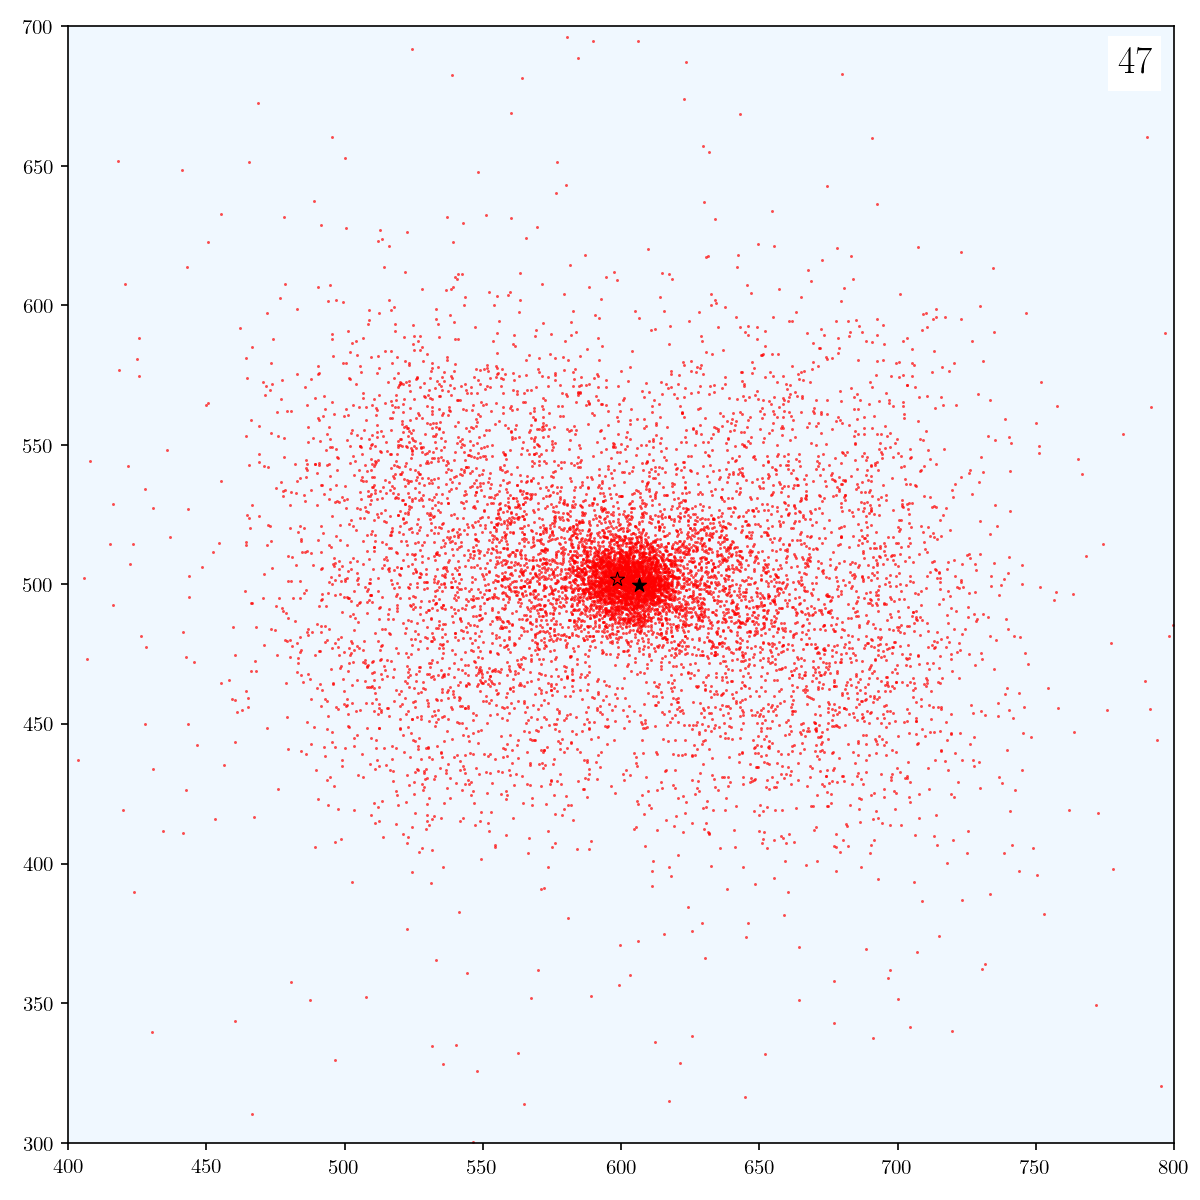
\includegraphics[width = 5.3cm]{images/jumper-demo/particleplot_00047.png}} 	& 
%            {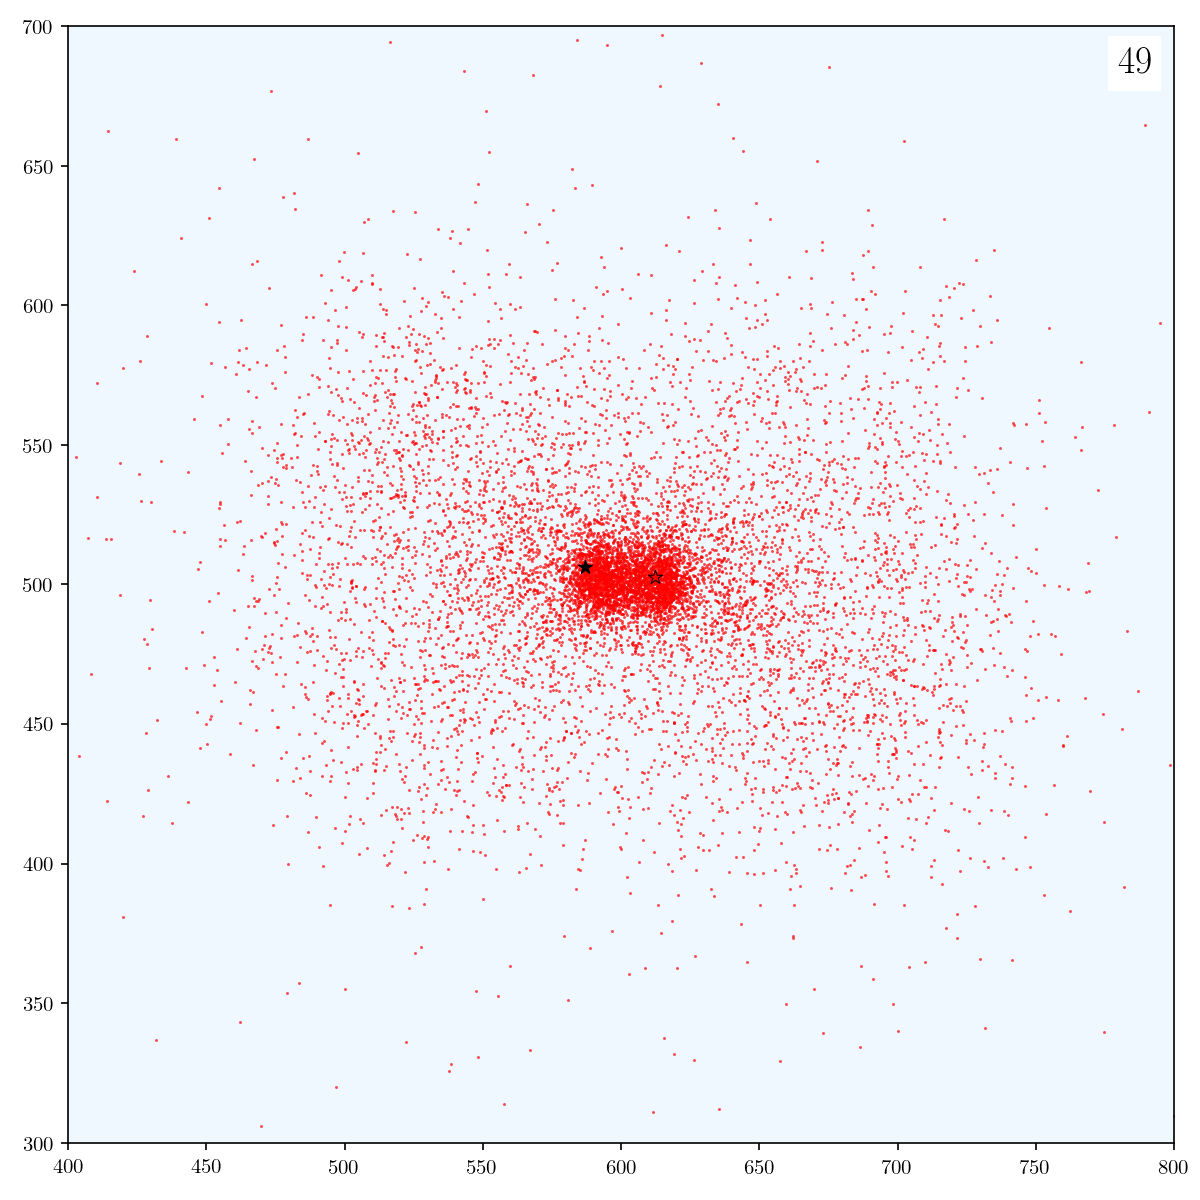
\includegraphics[width = 5.3cm]{images/jumper-demo/particleplot_00049.png}}  \\
        	\hline
    	\end{tabular}
    }
	\caption{\label{fig:jumper-demo} 
        Illustration of how haloes can seemingly merge into another one and re-appear a few snapshots later.
        The green and red particles are two initially distinct haloes that pass through each other.
        The galaxies assigned to them are marked by a star with the same colour as the particles.
        Black stars mark orphan galaxies, which have lost their unique host halo.
        The number in the upper right corner of each plot is the snapshot number that is depicted.
        In snapshots 27-31, the halo-finding algorithm didn't identify both haloes as distinct objects.
        However by tracking the red halo's orphan galaxy, it was possible to link the halo in snapshot 32 all the way back to snapshot 26.\\        
        The simulation was created using \texttt{DICE} \parencite{DICE}.
        Both haloes are identical with mass of $5\cdot 10^{10}\msol$, each containing 5000 particles and following a NFW mass profile.
        The plotted region corresponds to $400$ kpc on each side.
        }
\end{figure}




























































%\begin{sidewaysfigure}[!htbp]
%	{\renewcommand{\arraystretch}{0.1}
%		
%	\subfloat[The results of \phewon\ and \simple\ unbinding of the \ds-dataset: All particles, halo-namegiver particles only and subclumps particles only.]{
%		\begin{tabular}{|p{1cm} c c c|}
%			\hline
%			&&&\\[1em]
%													&
%			\textbf{All particles} 					&
%			\textbf{Halo-namegiver particles only} 	&
%			\textbf{Subhalo particles only} 		\\[1em]
%			%
%			%
%			\begin{sideways}{\hspace{3cm} \phewon}\end{sideways} \hspace*{-1em}%		 
%			& {\includegraphics[width = .28\textwidth]{images/dice-sub/dice-sub-plot-halo1-phew.png}} \hspace*{-1em}%
%			 & {\includegraphics[width = .28\textwidth]{images/dice-sub/dice-sub-halo-only-phew.png}} \hspace*{-1em}% 
%			 &{\includegraphics[width = .28\textwidth]{images/dice-sub/dice-sub-plot-subclumps-phew.png}} \\
%			%
%			%
%			\begin{sideways}{ \hspace{3cm}\simple\ unbinding }\end{sideways}	 \hspace*{-1em}			 &
%			{\includegraphics[width = .28\textwidth]{images/dice-sub/dice-sub-plot-halo1-nosaddle.png}} \hspace*{-1em}&
%			{\includegraphics[width = .28\textwidth]{images/dice-sub/dice-sub-halo-only-nosaddle.png}} \hspace*{-1em}&
%			{\includegraphics[width = .28\textwidth]{images/dice-sub/dice-sub-plot-subclumps-nosaddle.png}} \\
%			\hline
%		\end{tabular}
%		\label{fig:dice_sub_results_a}
%		}
%	}
%	\phantomcaption
%\end{sidewaysfigure}
%%=================================================
%%=================================================
%%=================================================
%\begin{sidewaysfigure}[!htbp]\ContinuedFloat
%	\footnotesize
%	{\renewcommand{\arraystretch}{0.1}
%	\subfloat[The results of \neigh\ and \iter\ unbinding of the \ds-dataset: All particles, halo-namegiver particles only and subclumps particles only.]{
%		\begin{tabular}{|p{1cm} c c c|}
%			\hline
%			&&&\\[1em]
%													&
%			\textbf{All particles} 					&
%			\textbf{Halo-namegiver particles only} 	&
%			\textbf{Subhalo particles only}			\\[1em]
%			%
%			%
%			\begin{sideways}{ \hspace{3cm}\neigh\ unbinding }\end{sideways}		\hspace*{-1em}		 &		
%			{\includegraphics[width = .28\textwidth]{images/dice-sub/dice-sub-plot-halo1-saddle.png}}\hspace*{-1em} &
%			{\includegraphics[width = .28\textwidth]{images/dice-sub/dice-sub-halo-only-saddle.png}}\hspace*{-1em} &
%			{\includegraphics[width = .28\textwidth]{images/dice-sub/dice-sub-plot-subclumps-saddle.png}} \\
%	%		%
%	%		%
%			\begin{sideways}{\hspace{3cm} \iter\ unbinding }\end{sideways}		\hspace*{-1em}		 &		
%			{\includegraphics[width = .28\textwidth]{images/dice-sub/dice-sub-plot-halo1-iter.png}} \hspace*{-1em}&
%			{\includegraphics[width = .28\textwidth]{images/dice-sub/dice-sub-halo-only-iter.png}} \hspace*{-1em}&
%			{\includegraphics[width = .28\textwidth]{images/dice-sub/dice-sub-plot-subclumps-iter.png}} \\
%			%
%			%
%			\hline
%		\end{tabular}
%		\label{fig:dice_sub_results_b}
%		}
%	}
%	\caption{
%	The results of different unbinding methods on the \dt-dataset.
%	}
%	\label{fig:dice_sub_results}
%\end{sidewaysfigure}
%
%

When a sub-halo travels towards the core of its parent halo, it will
merge with the central clump and disappear from the sub-halo lists.  It
can however re-emerge at a later snapshot and will be added back
to the list as a newly born halo. Such a scenario is shown in
Figure~\ref{fig:jumper-demo}.  Indeed, when this occurs, the merger
tree code will deem the sub-halo to have merged into the main halo, and
will likely find no progenitor for the re-emerged sub-halo, thus
treating it as newly formed.

This is a problematic case because we lose track of the growth history
of the sub-halo, regardless of its size, and massive clumps may be
found to just appear out of nowhere in the simulation.  This is a well
known problem for configuration-space halo finders
\citep{onionsSubhaloesGoingNotts2012}, and phase-space halo finders
like \texttt{ROCKSTAR} \citep{behrooziRockstarPhaseSpaceTemporal2013}
have been developed precisely to alleviate this issue.  While they
typically perform better than configuration-space halo finders,
\cite{SUSSING_COMPARISON} found that phase-space halo finders aren't
infallible in recovering all such missing haloes, and strongly
recommend checking for links between progenitors and descendants in
non-consecutive snapshots as well.

As our merger tree code works on the fly, future snapshots will not be
available at the time of the merger tree analysis, so it will be
necessary to check for progenitors of a descendant across multiple
snapshots.  This can be achieved by keeping track of the most bound
particles of each clump when it is merged into some other clump.
These tracer particles are also used to track {\it orphan galaxies}.
\footnote{In the context of SAM, orphan galaxies are galaxies born at
the center of dark matter haloes that merged later into bigger haloes
and eventually dissolved due to over-merging. As a consequence, these
galaxies don't have a parent halo or sub-halo anymore.}  For this
reason, we call these tracer particles ``orphan particles'', and
progenitor-descendant links over non-adjacent snapshots ``jumpers''.

These jumper links between different haloes widely separated in time
are less reliable than proper links between progenitors and
descendants from adjacent snapshots.  As we will discuss
in Section~\ref{chap:testing-nmb}, the quality of the merger trees
increases with the number of tracer particles used.  Using jumpers
corresponds to using only one tracer particle over a large time interval,
much larger than the one between two adjacent snapshots.

For this reason, priority is given to direct progenitor candidates in
adjacent snapshots.  Only if no direct progenitor candidates have been
found for some descendant, then progenitor candidates from
non-adjacent snapshots are searched for.  Because these progenitors
from non-adjacent snapshots are only tracked by one single particle,
we don't use the merit function to rank them.  Instead, we find the
orphan particle within the descendant clump which is the most tightly
bound.

In conclusion, although not ideal, using jumpers remains a necessity
to track these temporary merger events.  As a bonus, it allows us to
track orphan galaxies as will be discussed in
Section~\ref{chap:mock_catalogues}.





%============================================
\section{Details Of Our New Algorithm}
%============================================

The first step is to identify plausible progenitor candidates for
descendant clumps, as well as descendant candidates for progenitor
clumps.  In our algorithm, this is done by tracking tracer particles
across simulation snapshots. Tracer particles are selected within the
list of all particles belonging to the clump, ranked from most bound
to least bound. Indeed, the most bound particles are expected to
remain well within the clump boundary between two snapshots.  The main
parameter of our method is the maximum number of these tracer particle
used per progenitor clump, called $n_{\rm mb}$.  The minimum number of
tracer particles is obviously equal to $n_{\rm min}$, the minimum mass
threshold adopted by the \phew\ clump finder.

For every clump in the current snapshot, the $n_{\rm mb}$
most bound tracer particles are found and written to file.  In the following
output step, those files will be read in and the tracer particles
will be used to determine which clumps in the previous snapshot are the progenitors
of the clumps of the current snapshot.
 
As explained earlier, the main progenitor of each descendant and the
main descendant of each progenitor need to be found.  This search is
performed iteratively.  A main progenitor-descendant pair is
established when the main progenitor of a descendant is the main
descendant of said progenitor.  At every iteration, all descendant
candidates of all progenitors that haven't found their match yet are
checked. The descendants without a matching progenitor however only
move on to the next best progenitor candidate.  This is how we deal
with fragmentation events (see Section~\ref{sect:frag}).  For both
descendants and progenitors, all candidates are ranked from ``best''
to ``worst'' based on the merit function we have introduced before and
that we describe now in more details.

\subsection{The Merit Function}

Let $\mathcal{M}_{\rm pd}(A,B_i)$ be the merit function to be
maximised for a list of descendant candidates $B_i$ of a progenitor
$A$. Let $n_{\rm mb}$ be the total number of particles of progenitor
$A$ that are being traced. Note that $n_{mb}$ can be smaller than the
total number of particles in clump $A$.  A straightforward ansatz for
the merit function would be to based on the fraction of particle traced from the
progenitor to the descendant candidate:
\begin{equation}
\mathcal{M}_{\rm pd}(A,B_i) \propto \frac{n_{A \cap B_i}}{n_{\rm mb}}
\end{equation}
where $n_{A \cap B_i}$ is the number of tracer particles of $A$ found
in $B$.  Similarly, we define $\mathcal{M}_{\rm dp}(A_i,B)$ as the
merit function to be maximised for a list of progenitor candidates
$A_i$ of a descendant $B$. Another straightforward ansatz would be
based on the fraction of particle traced from the progenitor
candidates to the descendant:
\begin{equation}
\mathcal{M}_{\rm dp}(A_i,B) \propto \frac{n_{A_i \cap B}}{n_B}
\end{equation}
where $n_B$ is the total number of particles in the descendant $B$.
In these two merit functions, $n_{\rm mb}$ and $n_B$ are just
normalizing factors. They are independent of the properties of the
candidate and hence won't affect the selection process.  We can
therefore merge these two merit functions into one, defined as
\begin{equation}
\mathcal{M}(A,B) \propto n_{A \cap B}
\end{equation}

The \phew\ clump finder in \ramses\ identifies the main halo as the
clump with the highest density maximum.  During a major merger event,
the halo will have two clumps with similar masses and comparable
maximum densities.  It is then quite common that small variations in
the value of the density maxima will cause the identification of the
main halo to jump between these two clumps.  Indeed, the particle
unbinding algorithm will identify particles that are not bound to the
sub-halo and pass them on to the main halo, modifying the resulting
mass for the two clumps.  This effect is particularly strong if one
uses the {\it strictly bound} definition for the particle
assignment. As a consequence, because the identification of the main
halo varies, strong mass oscillations are expected. To counter this
spurious effect, we modify the merit function to preferentially select candidates with
similar masses:
\begin{equation}
\mathcal{M}(A,B) = \frac{n_{A \cap B}}{n_{\rm max} - n_{\rm min}} \label{eq:merit}
\end{equation}
where $n_{\rm max}=\max(n_A,n_B)$ and $n_{\rm min}=\min(n_A,n_B)$.  An
overview of other merit functions used in the literature is given in
Table~1 of \cite{SUSSING_COMPARISON}.

\subsection{Final Linking Process}

The iteration is repeated until every descendant has been checked
against every progenitor. Finally, the links in the tree making
process are established following these two steps:

\begin{enumerate}
  
\item Progenitors that have not found any available descendant will be
  considered to have merged into their highest ranked descendant
  candidate.  These progenitors are recorded in the merger tree as
  {\it merged progenitors}.  In this case, only one tracer particle is
  kept for future use, the most bound particle in the list of $n_{\rm
    mb}$ tracer particles.  This single particle is referred to as the
  \emph{orphan particle} of the merged progenitor.  It is used to
  check whether the merger event was a final merger or only a
  temporary merger. It is also used to track orphan galaxies.

\item Descendants that have not found any available progenitor will be
  checked against non-consecutive past snapshots. The particles of the
  descendant are compared to the orphan particles in the list of past
  merged progenitors\footnote{There is an option to remove past merged
  progenitors from the list if they have merged into their main
  descendant too many snapshots ago.  By default, however, the
  algorithm will store them all until the very end of the
  simulation.}.  The most strongly bound orphan particle will be used
  to restore the broken link with its main progenitor.  Finally,
  remaining descendants without a progenitor are considered as being
  newly formed.

\end{enumerate}
  
For the interested reader, an even more detailed description of the merger tree
algorithm is given in Appendix~\ref{app:detailed_mergertree}.


    %\begin{figure}[htb]
%	\centering
%	\fbox{\includegraphics[width = .8\textwidth ]{images/cosmo/cos-part2map-npart.png}}%
%	\caption{
%		The particle distribution of the \cosmo\ dataset.
%		It is a cosmological simulation of $128^3$ dark matter particles at redshift $z=0$ with $H_0 = 70.4$ and density parameters $\Omega_m = 0.272$ and $\Omega_\Lambda=0.728$.
%	}%
%	\label{fig:cosmo_origin}
%\end{figure}




%\begin{figure}[htbp!]
%	\centering
%	\minipage[t]{0.497\textwidth}
%	\centering
%	\fbox{\includegraphics[height=\textwidth]{images/dice-two/dice-two-original-plot.png}}%
%	\caption{
%		The initial particle distribution of the \dt\ dataset. A smaller halo (subhalo 1) made of 40'000 particles is nested within a bigger halo (halo-namegiver), which contains 200'000 particles.
%	}%
%	\label{fig:dice_two_origin}
%	\endminipage%\hspace{.1cm}
%	\hspace*{\fill}
%	%
%	\minipage[t]{0.497\textwidth}
%	\centering
%	\fbox{\includegraphics[height=\textwidth, keepaspectratio]{images/dice-sub/dice-sub-original-plot.png}}%
%	\caption{
%		The initial particle distribution of the \ds\ dataset. 3 small halos (subsubhalo 1-3), made of 20'000 particles, are around a bigger halo (subhalo 1), which contains 200'000 particles. These four structures are then enveloped by an even bigger halo (halo-namegiver), made of 1'000'000 particles.
%	}%
%	\label{fig:dice_sub_origin}
%	\endminipage\hspace*{\fill} 
%\end{figure}


%============================================================================
\subsection{Testing Parameters of the Merger Tree Algorithm}\label{chap:tests}
%============================================================================

%============================================================================
\subsubsection{Methods}
%============================================================================
The current implementation of the merger tree algorithm allows for multiple free parameters for the user to choose from, which will be introduced and tested further below in this section.
Testing these parameters is not a straightforward matter, mainly because there is no ``correct solution'' which would enable a comparison and error quantification.
Nevertheless, one could define a set of quantities one deems a priori favourable for a merger tree and cross-compare these quantities obtained for varying parameters on an identical cosmological simulation.
This method was also used in the ``Sussing Merger Trees Comparison Project'' (\cite{SUSSING_COMPARISON}, \cite{SUSSING_CONVERGENCE}, \cite{SUSSING_HALOFINDER}).
Some or similar quantifications from the ``Sussing Merger Tree'' paper series are adapted in this work, as they seem sensible and even allow for a rough cross-comparison with other merger tree codes.

The following properties will be used to quantify the merger trees:

\begin{itemize}
	\item \textbf{Length of the Main Branch}
	
		The length of the main branch of $z=0$ haloes gives a most basic measure of how far back in time the formation history of these haloes can be tracked.
		Naturally, longer main branches should be considered a favourable feature for a merger tree code.
		
		In this work, the length of the main branch is defined as the number of snapshots a halo and its progenitors appear in.
		A newly formed halo at the $z=0$ snapshot, which doesn't have any progenitors, will by definition have the main branch length of $1$.
		If a halo appears to merge into another, but re-emerges at a later snapshot and is identified to do so, then the snapshots where it is missing from the halo catalogue will still be counted towards the length of the main branch as if it weren't missing. \\

	
	\item \textbf{Branching Ratio}
	
		A further simple tree quantity is the number of branches of the tree.
		The main branch is included in this count, thus the minimal number of branches for each clump at $z=0$ will be $1$.
	
%		Even though the evaluation will be conducted on the identical simulation, some parameters will effect the definitions of haloes an therefore the resulting halo catalogues.
%		As the evaluation will be conducted on the same simulation, I expect lower branching ratios to be accompanied by longer main branches and vice versa.
		As long as the halo catalogue remains unchanged, lower branching ratios mean less merging events and therefore should be accompanied by longer main branches. 
		
		In the picture of bottom-up structure formation, where larger object form through repeated mergers of smaller ones, one would expect more massive clumps to have longer main branches and a higher branching ratio. \\
		
		
	
	\item \textbf{Misidentifications, Quantified by Displacements}
	
		Since no unique correct solution exists, the same displacement statistic $\Delta_r$ as is done in \cite{SUSSING_CONVERGENCE} to quantify misidentifications is used:
%	
		\begin{align}
			\Delta_r = \frac{
				| \mathbf{r}_{k+1} - \mathbf{r}_k - 0.5 (\mathbf{v}_{k+1} + \mathbf{v}_k) (t_{k+1} - t_k) |}
				{0.5(R_{200,k} + R_{200,{k+1}} + | \mathbf{v}_{k+1} + \mathbf{v}_k | (t_{k+1} - t_k)} \label{eq:displacements}
		\end{align}
%
		where $\mathbf{r}_{k+1}$, $\mathbf{v}_{k+1}$ and $\mathbf{r}_k$, $\mathbf{v}_k$ are the position and velocity of a clump at snapshot $k+1$ and its progenitor at snapshot $k$, respectively; $t_{k+1}$ and $t_k$ are the cosmic times at which the two clumps were defined, and $R_{200}$ is the radius that encloses an overdensity of 200 times the critical density $\rho_{c} = \frac{3 H^2}{8 \pi G}$.
		
		It can be interpreted as the difference between the actual displacement $(\mathbf{r}_{k+1} - \mathbf{r}_k)$ and the expected one $(0.5 (\mathbf{v}_{k+1} + \mathbf{v}_k) (t_{k+1} - t_k) )$, normalized by an estimate of how large the displacement is allowed to be to rule out a clear misidentification.
		This estimate is the sum of the average halo size, $0.5(R_{200,k}+R_{200,k+1})$, allowing the exact clump position to vary within its own boundaries, and an estimate for the distance travelled based on the time interval and average velocities, $0.5| \mathbf{v}_{k+1} + \mathbf{v}_k | (t_{k+1} - t_k)$.
		
		Values of $\Delta_r > 1$ would indicate a misidentification, so the parameters minimising $\Delta_r$ should be preferred, provided the acceleration is approximately uniform.
		This is often not the case for subhaloes, which will shift the distribution of $\Delta_r$ towards higher values. 
		Nevertheless, it is used for subhaloes as well, since the goal is a simple cross-comparison of varying parameters, hoping to get some indication towards which parameters produce the most reliable merger trees. \\
		
		
		
		
	\item \textbf{Logarithmic Mass Growth}
	
		The logarithmic mass growth rate of haloes is approximated discretely by
		%
		\begin{align}
			\frac{\de \log M}{\de \log t} \approx \frac{(t_{k+1}+t_{k})(M_{k+1} -M_{k})}{(t_{k+1} - t_k)(M_{k+1} + M_{k})} \equiv \alpha_M(k, k+1)
		\end{align}
		%
		where $k$ and $k+1$ are a clump and its descendant, with masses $M_k$ and $M_{k+1}$ at times $t_k$ and $t_{k+1}$, respectively.
		
		To reduce the range of possible values to the interval $(-1, 1)$, \cite{SUSSING_CONVERGENCE} define
		%
		\begin{align}
			\beta_M = \frac{2}{\pi}\arctan(\alpha_M) \label{eq:massgrowth}
		\end{align}
		%
		Within the hierarchical structure formation scenario, one would expect haloes to grow over time, thus a distribution of $\beta_M$ should be skewed towards $\beta_M > 0$.
        $\beta_M \rightarrow \pm 1$ imply $\alpha_M \rightarrow \pm \infty$, indicating extreme mass growth or losses.\\
		
	\item \textbf{Mass Growth Fluctuations}
		
		Mass growth fluctuations can be quantified by using
		%
		\begin{align}
			\xi_M = \frac{\beta_M(k, k+1) - \beta_M(k-1, k)}{2} \label{eq:massfluct}
		\end{align}
		%
		where $k-1$, $k$, $k+1$ represent consecutive snapshots.
		When far from zero, it implies an extreme growth behaviour. 
        For $\xi_M\rightarrow \pm 1$, $\beta_M(k, k+1) \rightarrow \pm 1$ and $\beta_M(k-1, k) \rightarrow \mp 1$, indicating extreme mass loss followed by extreme mass growth for the upper sign, and the opposite behaviour for the lower sign.
		Within the hierarchical structure formation scenario this behaviour shouldn't occur and such an occurrence might indicate either a misidentification by the tree code or an error in the mass assignment of the halo finder.
\end{itemize}



%In order to produce evaluations that will be comparable to \cite{SUSSING_CONVERGENCE}, only clumps with mass above $5 \cdot 10^{11} \msol$ will be considered for the displacement, mass growth and mass growth fluctuation statistics.
%In all cases that will be considered, more than 3000 clumps have masses above this mass threshold.




In the evaluation, no distinction between main haloes and subhaloes is made.
Distinguishing between those two cases gives no information on which parameters are preferable that can't already be seen when no distinction is made, so for clarity's sake, the evaluations for main haloes and subhaloes individually are omitted from the main body of this work, but the figures for the displacement statistics, logarithmic mass growth and mass growth fluctuations for haloes and subhaloes separately can be found in appendix \ref{app:halo-subhalo-mtree-evals}.
















%============================================================================
\subsubsection{Parameters Influencing the Halo Catalogue}
%============================================================================

In the current implementation, there are two parameters which influence the halo catalogue aside from mass and density thresholds.
The first one concerns the mass definition of a subhalo.
By construction, the mass of a halo contains all its substructure's mass.
This isn't necessarily the case for subhaloes though.
In a hierarchical structure formation scenario, substructures are expected to contain substructures on their own.
Whether to recursively include substructure mass to their respective parent structure is a matter of choice and application. 
The influence of this choice on the merger trees is shown in figures \ref{fig:saddle_nosaddle_masses}, \ref{fig:saddle_nosaddle_mbl_nbranch} and \ref{fig:saddle_nosaddle_displacement}.
When subhaloes' masses are defined to include their respective substructure masses, the results will be labelled as \inc, or \exc\ otherwise.




A second matter of definition is in which case a particle is to be considered as bound to a clump.
The concept of ''exclusively bound`` particles, which aren't allowed to leave the spatial boundaries of their host clump, was introduced in section \ref{chap:unbinding}.
It is to be expected that demanding particles to be exclusively bound will find more unbound particles than not doing so, thus changing the subhalo catalogue.

The influence of this choice on the merger trees is also shown in figures \ref{fig:saddle_nosaddle_masses}, \ref{fig:saddle_nosaddle_mbl_nbranch}, and \ref{fig:saddle_nosaddle_displacement}, along with the influence of the previously described \inc\ and \exc\ mass definitions.
When bound particles are allowed to leave the clump's boundaries, the results will be labelled as \nosad, or \sad\ otherwise.







%============================================================================
\subsubsection{Dataset Used for Testing}
%============================================================================
All tests are performed on the same dark matter only simulation which contains $256^3 \approx 1.7\cdot 10^7$ particles of identical mass $m_p = 1.55\cdot 10^9\msol$. 
The Hubble constant $H_0 = 70.4$ km s$^{-1}$Mpc$^{-1}$ and density parameters $\Omega_m = 0.272$ and $\Omega_\Lambda = 0.728$ were used. 
The density threshold for clump finding was chosen to be 80$\rho_c$  and the saddle threshold for halos was set to 200$\rho_c$, where $\rho_c = \frac{3 H^2}{8 \pi G}$ is the cosmological critical density. 
Only clumps with at least 10 particles were kept.

The output strategy was chosen as follows:
As virtually no haloes were found before $a\leq 0.1$, only few snapshots were stored up to $a=0.1$ in steps of $\Delta a \approx 0.02$.
From this point on, snapshots were created every $\Delta t \approx 0.3$ Gyrs up until $a = \tfrac{1}{3}$, after which a smaller time interval of $\Delta_t \approx 0.2$ Gyrs were chosen.
This choice resulted in 67 snapshots to get to $z = 0$.
The simulation was then continued for 3 further snapshots with $\Delta t \approx 0.2$ Gyrs to ensure that the merging events at $z = 0$ are actually mergers and not clumps that will re-emerge later.

A visualisation of the merger tree of the most massive main halo of this simulation is shown in figure \ref{fig:mergertree}.
Stunningly, even for a relatively low resolution simulation like the one used, incredibly complex formation histories can be uncovered and followed back to the first snapshot with identifiable haloes.
Note that this is only the tree of the central halo, not containing any subhaloes that are still identifiable as such.


\begin{figure}[H]
    \begin{minipage}[c]{0.6\textwidth}
    	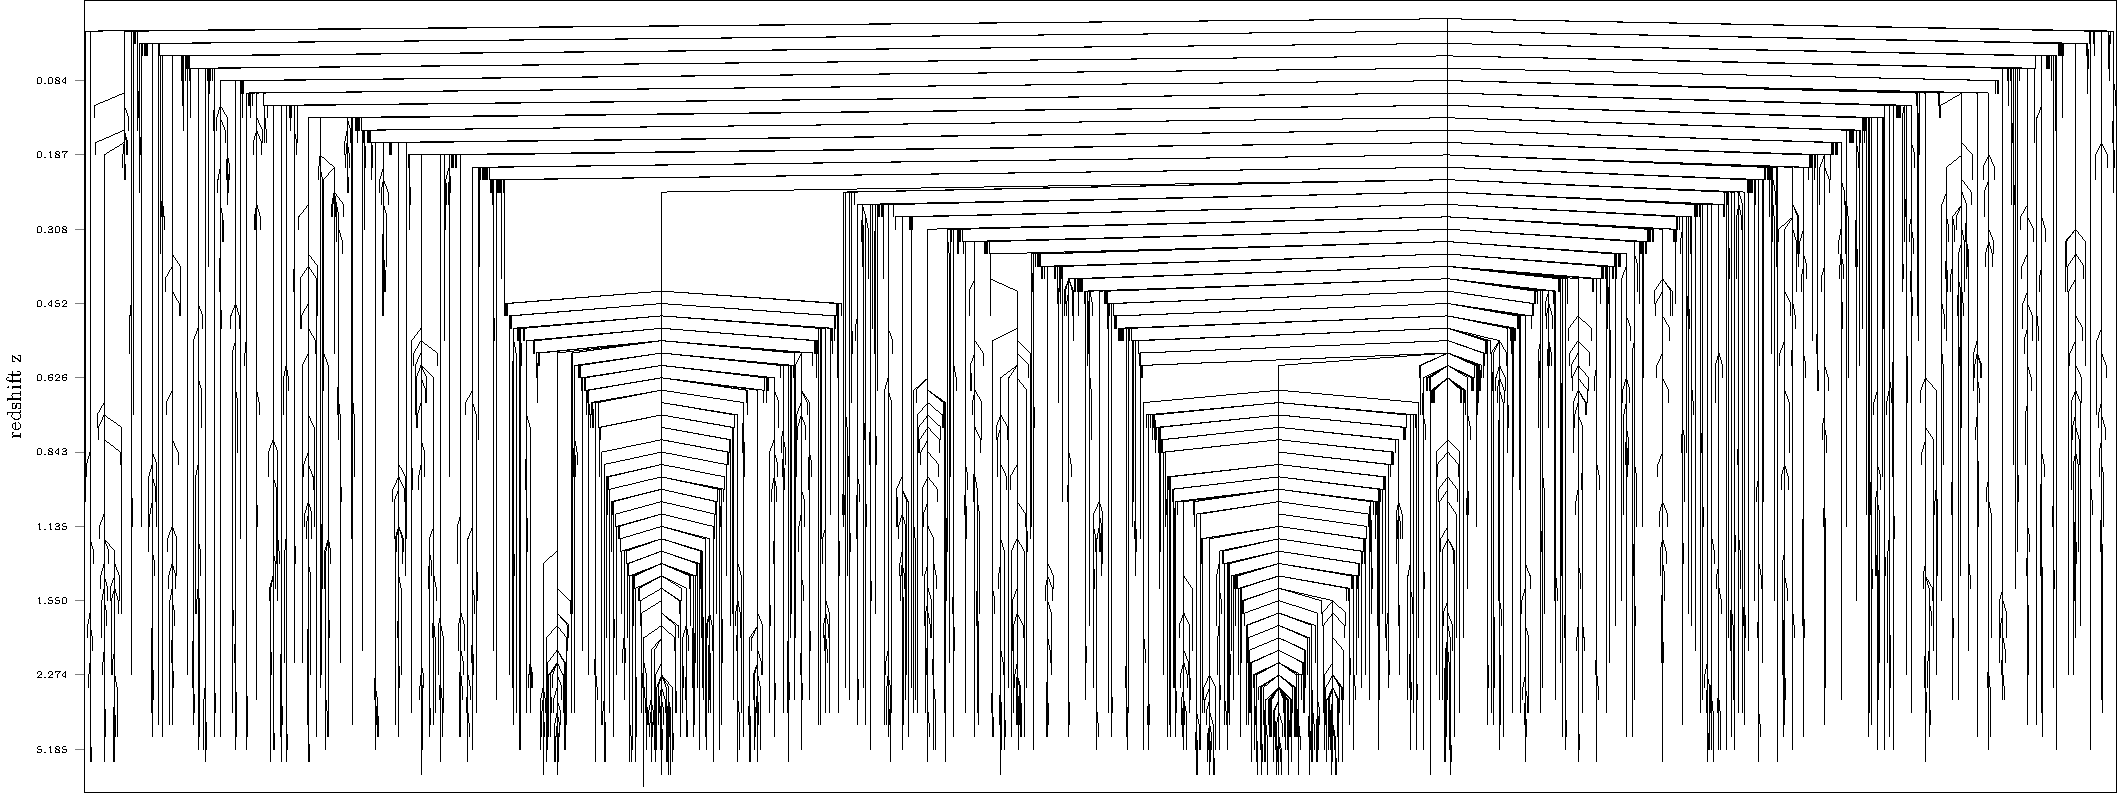
\includegraphics[width=25cm, keepaspectratio,angle=90,origin=c]{images/mergertree.pdf}%
    \end{minipage}\hfill
    \begin{minipage}[c]{0.4\textwidth}
    	\caption{
    		The merger tree of the most massive central halo in the simulation, obtained with the parameters \exc\ and $n_{mb}=1000$.
    		The redshift at the time of the snapshot is given on the $x$-axis, the $y$-axis has no physical meaning.
    	}%
    	\label{fig:mergertree}
    \end{minipage}
\end{figure}









\subsubsection{Influence of the Definition of Subhalo Mass}


\begin{figure}[H]
	\centering
	\includegraphics[width=\textwidth, keepaspectratio]{images/saddle-vs-nosaddle/mass_growth_and_fluctuation.pdf}%
	\caption{
		Logarithmic mass growth and mass growth fluctuation distributions for progenitor - descendant pairs or three consecutive nodes in a branch, respectively, with masses above $5\cdot 10^{11}\msol$ throughout the entire simulation for the halo catalogue influencing parameters: 
		whether subhalo particles are included (\inc) or excluded (\exc) in the clump mass of satellite haloes, and whether to consider particles which might wander off into another clump as bound (\nosad) or not (\sad).
		The distribution is computed as a histogram which is normalised by the total number of events found.
	}%
	\label{fig:saddle_nosaddle_masses}
\end{figure}

\begin{figure}[p]
	\centering
	\minipage[t]{0.49\textwidth}
	\centering
	\includegraphics[width=\textwidth]{images/saddle-vs-nosaddle/length_of_main_branch.pdf}
	\endminipage%\hspace{.1cm}
	\hspace*{\fill}
	%
	\minipage[t]{0.49\textwidth}
	\centering
	\includegraphics[width=\textwidth, keepaspectratio]{images/saddle-vs-nosaddle/number_of_branches.pdf}%
	\endminipage\hspace*{\fill} 
	\caption{
		Length of main branches, defined as the number of snapshots this clump appears in, and the number of branches including the main branch, for the halo catalogue influencing parameters of $z=0$ clumps: 
		whether subhalo particles are included (\inc) or excluded (\exc) in the clump mass of satellite haloes, and whether to consider particles which might wander off into another clump as bound (\nosad) or not (\sad).
		Four distributions are shown, for four different ranges of numbers of particles at $z=0$ exclusively assigned to the clump: less then 100 (top), 100-500, 500-1000 and more than 1000 (bottom), where each particle has mass $m_p = 1.55 \cdot 10^9 \msol$.
		The distribution is computed as a histogram which is normalised by the total number of events found per particle count group.
	}%
	\label{fig:saddle_nosaddle_mbl_nbranch}
\end{figure}

\begin{figure}[H]
	\centering
	\minipage[t]{0.49\textwidth}
		\includegraphics[width=\textwidth]{images/saddle-vs-nosaddle/displacements.pdf}%
		\caption{
			Distribution of the displacements for progenitor - descendant pairs with masses above $5\cdot 10^{11}\msol$ throughout the entire simulation for the halo catalogue influencing parameters: 
			whether subhalo particles are included (\inc) or excluded (\exc) in the clump mass of satellite haloes, and whether to consider particles which might wander off into another clump as bound (\nosad) or not (\sad).
			The distribution is computed as a histogram which is normalised by the total number of events found.
		}%
		\label{fig:saddle_nosaddle_displacement}
	\endminipage%\hspace{.1cm}
	\hspace*{\fill}
	%
	\minipage[t]{0.49\textwidth}
		\centering
		\includegraphics[width=\textwidth]{images/ntracers/displacements.pdf}%
		\caption{
			Distribution of the displacements for progenitor - descendant pairs with masses above $5\cdot 10^{11}\msol$ throughout the entire simulation for varying numbers of clump tracer particles $n_{mb}$.
			The distribution is computed as a histogram which is normalised by the total number of events found.
		}%
		\label{fig:ntracers_displacement}
	\endminipage
\end{figure}













%===============================================================
%\subsubsection*{Length of Main Branch and Branching Ratio}
%===============================================================

\begin{table*}
	\caption{
        Average data for all clumps at $z=0$ depending on whether to consider particles which might wander off into another clump as bound (\nosad) or not (\sad).
        The results shown are for the \exc\ mass definition, which show no significant difference to when the \inc\ mass definition is used.
%        The groups I, II, III and IV are defined as clumps that contain less then 100, 100-500, 500-1000 or more than 1000 particles, respectively.
        \label{tab:saddle_nosaddle}
    }
        
%	{\small 
%		\begin{tabular}[c]{l | p{2.8cm} | p{2.8cm} |}
%													&	 \sad\  &   \nosad\ \\ 
%			
%			\hline
%			%
%			total clumps	 						&	 16262	& 	17242 	\\			
%			%		
%%			max number of particles in a clump 		&	 414570	& 	271438 	\\			
%			%		
%			median number of particles in a clump 	&	 83		& 	93 		\\			
%			%
%			\hline
%			%		
%			average main branch length group I		&	23.153	& 	20.527 	\\			
%			%
%			average main branch length group II		&	48.835	& 	48.642 	\\			
%			%		
%			average main branch length group III	&	54.715	& 	54.904 	\\			
%			%
%			average main branch length group IV		&	53.958	& 	56.265 	\\			
%			%
%			\hline
%			%		
%			average number of branches group I		&	1.327	& 	1.230 	\\			
%			%
%			average number of branches group II		&	3.448	& 	3.603 	\\			
%			%		
%			average number of branches group III	&	8.670	& 	8.661 	\\			
%			%
%			average number of branches group IV		&	29.457	& 	28.607 	\\				
%			%
%			\hline	
%		\end{tabular}
%	}

	{\small 
		\begin{tabular}[c]{l | p{2.8cm} | p{2.8cm} |}
													&	 \sad\  &   \nosad\ \\ 
			
			\hline
			%
			total clumps	 						&	 16262	& 	17242 	\\			
			%		
%			max number of particles in a clump 		&	 414570	& 	271438 	\\			
			%		
			median number of particles in a clump 	&	 83		& 	93 		\\			
			%
			\hline
			%
			average main branch length & & \\
			%	
			clumps with < 100 particles		&	23.2	& 	20.5 	\\			
			%
			clumps with 100-500 particles	&	48.8	& 	48.6 	\\			
			%		
			clumps with 500-1000 particles	&	54.7	& 	54.9 	\\			
			%
			clumps with > 1000 particles	&	54.0	& 	56.3 	\\			
			%
			\hline
			average number of branches & & \\
			%		
			clumps with < 100 particles		&	1.3		& 	1.2 	\\			
			%
			clumps with 100-500 particles	&	3.4		& 	3.6 	\\			
			%		
			clumps with 500-1000 particles	&	8.7		& 	8.7 	\\			
			%
			clumps with > 1000 particles	&	29.5	& 	28.6 	\\				
			%
			\hline	
		\end{tabular}
	}
\end{table*}

In accordance to the hierarchic structure formation picture, more massive clumps tend to have longer main branches and a higher branching ratio in all cases.
This is clearly visible from the average length of the main branch and the average branching ratio of clumps at $z=0$, binned in four groups by their mass, which are given in table \ref{tab:saddle_nosaddle}.
The average main branch length for clumps with more that 500 particles is $\sim 55$, meaning that on average, haloes with mass above $\sim 7.75 \cdot 10^{11} \msol$ can be traced back to redshift $\sim 3$.

The length of the main branches for the same four mass bins of clumps are shown in figure \ref{fig:saddle_nosaddle_mbl_nbranch}.
Interestingly, small clumps with less than 100 particles seem to have a somewhat constant formation rate from $z \sim 2$ until $z \sim 0.2$.
Furthermore they too can be traced back to high redshifts, indicating good performance of the merger tree algorithm.

Whether subhalo masses are computed in an \exc\ or \inc\ manner seems to have negligible effect on the branching ratio and the length of main branch.

The \sad\ definition of bound particles however tends to result in longer main branch lengths for small clumps with less than 100 particles.
This might be explained by the fact that in general, when \sad\ is applied, subhaloes which are at the bottom of the clump hierarchy will tend to contain less bound particles compared to when \nosad\ is used, and have shorter lifetimes because they are found to have merged into their hosts earlier.
Therefore clumps with more than 100 particles with the \nosad\ condition might be moved to the lower mass bin of $\leq$ 100 particles when \sad\ is used, thus increasing the fraction of clumps with high main branch lengths (lengths of 50-60), as well as the number of branches.
Evidence of the earlier merging can be seen in the overall higher number of branches in the right column of figure \ref{fig:saddle_nosaddle_mbl_nbranch}, as well as the average values, total clump numbers and the median particle numbers in a clump given in table \ref{tab:saddle_nosaddle}.
%The longer main branch length can be understood by considering that with a clump definition which in general has less particles, some clumps which would otherwise be sorted in a higher mass bin are sorted in a lower one instead.
%This should increase both the length of main branches and the number of branches for lower mass clumps (below 100 particles) and decrease them for high mass clumps (above 1000 particles), as table \ref{tab:saddle_nosaddle} and figure \ref{fig:saddle_nosaddle_mbl_nbranch}.
%For intermediate masses, meaning 100-1000 particles in a clump, the distributions and average values don't vary significantly.








%==========================================
%\subsubsection*{Misidentifications}
%==========================================

The displacement statistic used to quantify misidentifications in figure \ref{fig:saddle_nosaddle_displacement} indicates that no parameter choice results in a obviously ``wronger'' progenitor-descendant pairing.
Even though there are some  $\Delta_r > 1$, indicating that there might be misidentifications present, it can't be determined easily whether they truly are.
When the displacement statistic is calculated for haloes and subhaloes separately, which is shown in appendix \ref{app:halo-subhalo-mtree-evals}, no halo descendant-progenitor pair shows a displacement above 1, indicating no obvious misidentifications, yet a significant fraction of subhalo progenitor-descendant pairs have a high displacement value $\Delta_r > 1$.
However, the displacement statistic is calculated assuming a uniform acceleration, which is not valid for subhaloes.
On the other hand, the fact that any parameter pair used found at least some clumps with more than 1000 particles at $z=0$ with main branch length of unity, which is the case when it doesn't have any progenitor, and thus essentially ``appearing out of nowhere'', is strongly suggesting present misidentifications.




%=========================================================================
%\subsubsection*{Logarithmic Mass Growth and Mass Growth Fluctuations}
%=========================================================================

The logarithmic mass growth in figure \ref{fig:saddle_nosaddle_masses} shows that as expected, the distribution is indeed skewed towards $\beta_M > 0$. 
When the \inc\ parameter is used, the distribution of mass growth contains a few more extreme mass growths and losses $(\beta_M \rightarrow \pm 1)$, as well as some high mass growth fluctuations $(\xi_M \rightarrow \pm 1)$ (see figure \ref{fig:saddle_nosaddle_masses}).
When the \nosad\ parameter is used, noticeably more extreme mass growth $(\beta_M \rightarrow \pm 1)$ and mass growth fluctuations $(\xi_M \rightarrow \pm 1)$ occur.






%==========================================
%\subsubsection*{Conclusion}
%==========================================
In conclusion, whether to use \inc\ or \exc\ mass definitions for subhaloes shows very little effect on the merger trees.
Based on the fewest extreme mass growth fluctuations, the \sad\ parameter is clearly preferable. 
%With \sad\ in use, the \exc\ parameter leads to less clumps over 1000 particles with main branch length of 1, and a little fewer extreme mass growths and fluctuations, which is why I conclude that the combination of \exc\ and \sad\ parameters should create the most reliable merger trees.





	













%===================================================================
\subsection{Influence of the Number of Tracer Particles Used}
%===================================================================

\begin{table}[ht]
	\begin{center}
		{\small 
		\begin{tabular}[c]{l | p{1cm} | p{1cm} | p{1cm} | p{1cm} | p{1cm} | p{1cm} | p{1cm} |}
			$n_{mb}=$								&	1 		& 	10 		& 	50 		& 	100 	& 200 	& 500 		& 1000 \\
			\hline
	%
%			total clumps at $z=0$					&	16262	& 	16262	& 	16262	&	16262 	& 16262  & 16262 	& 16262 \\
	%		
%			max NoP in a clump 		&	414570	& 	414570	& 	414570	&	414570 	& 414570 & 414570 	& 414570  \\ 	
	%		
%			median NoP in a clump 	&	83		& 	83		& 	83		&	83  	& 83	 & 83 	& 	83  \\	
	%
%			\hline
	%		
			average MBL group I		&	24.188	& 	24.330	& 	23.567	&	23.353 	& 23.153 & 22.876 	& 22.656  \\	
	%
			average MBL group II		&	50.399	& 	50.116	& 	49.472	&	49.122 	& 48.835 & 48.777 	& 48.762  \\	
	%		
			average MBL group III	&	55.233	& 	54.863	& 	53.264	&	54.059 	& 54.715 & 54.327 	& 54.165  \\	
	%
			average MBL group IV		&	56.690	& 	54.884 	& 	52.345	&	52.900 	& 53.958 & 55.761 	& 56.448  \\
	%
			\hline
	%		
			average NoB group I		&	1.228	& 	1.305	& 	1.296	&	1.305 	& 1.327  & 1.357 	& 1.367  \\	
	%
			average NoB group II		&	2.699	& 	3.062	& 	3.265	&	3.337 	& 3.448  & 3.586 	& 3.596  \\	
	%		
			average NoB group III	&	6.625	& 	7.229	& 	8.051	&	8.206 	& 8.670  & 8.914 	& 9.121  \\	
	%
			average NoB group IV		&	20.407	& 	25.237	& 	27.288	&	28.554 	& 29.457 & 30.443 	& 31.420  \\	
	%
			\hline	
		\end{tabular}
		}
	\caption{
		Average data for all clumps at $z=0$ for varying numbers of clump tracer particles $n_{mb}$. 
		The groups I, II, III and IV are defined as clumps that contain less then 100, 100-500, 500-1000 or more than 1000 particles, respectively.
		``MBL'' is an abbreviation for ``main branch length'', ``NoB'' stands for ``number of branches''.
        % ``NoP'' for ``number of particles''.
		}
	\label{tab:ntracers}
	\end{center}	
\end{table}
\begin{table}[ht]
	\begin{center}
		{\small 
		\begin{tabular}[c]{l | p{1cm} | p{1cm} | p{1cm} | p{1cm} | p{1cm} | p{1cm} | p{1cm} |}
			$n_{mb}=$								&	1 		& 	10 		& 	50 		& 	100 	& 200 	& 500 	& 1000  \\
			\hline	
			trees pruned from tree catalogue		&	33924	&	23091	&	22146	& 	22131 	& 22130 & 22129 & 22129 \\	
	%
			highest particle number of a LIDIT		&	1369	&	236		&	236		&	236 	& 236 	& 157 	& 157  	\\	
	%
			median particle number of a LIDIT		&	19		&	20		&	20		&	20 		& 20 	& 20 	& 20  	\\
	%
			LIDITs with >100 particles pruned 		&	513		&	42		&	32		&	26 		& 25 	& 24 	& 24  	\\
    %
            total number of jumpers                 &  20176    &   20905   &   22074   &   22041   & 20970 & 19307 & 18249 \\
			\hline
		\end{tabular}
		}
	\caption{
		Trees pruned from the merger tree catalogue for varying numbers of clump tracer particles $n_{mb}$ throughout all snapshots. 
		``LIDIT'' is an abbreviation of ``last identifiable descendant in tree''. 
		For LIDITs no further descendants could be identified throughout the simulation and consequently their tree was pruned from the merger tree catalogue.
        A ``jumper'' refers to a clump that has been merged into another clump at some snapshot, but re-emerged at a later snapshot, like shown in figure \ref{fig:jumper-demo}.
		}
	\label{tab:ntracers-pruning}
	\end{center}	
\end{table}

\begin{figure}[H]
	\centering
	\includegraphics[width=\textwidth, keepaspectratio]{images/ntracers/mass_growth_and_fluctuation.pdf}%
	\caption{
		Logarithmic mass growth and mass growth fluctuation distributions for progenitor - descendant pairs or three consecutive nodes in a branch, respectively, with masses above $5\cdot 10^{11}\msol$ throughout the entire simulation for varying numbers of clump tracer particles $n_{mb}$.
		The distribution is computed as a histogram which is normalised by the total number of events found.
	}%
	\label{fig:ntracers_masses}
\end{figure}

\begin{figure}[p]
	\centering
	\minipage[t]{0.49\textwidth}
	\centering
	\includegraphics[width=\textwidth]{images/ntracers/length_of_main_branch.pdf}
	\endminipage%\hspace{.1cm}
	\hspace*{\fill}
	%
	\minipage[t]{0.49\textwidth}
	\centering
	\includegraphics[width=\textwidth, keepaspectratio]{images/ntracers/number_of_branches.pdf}%
	\endminipage%\hspace*{\fill}
	\caption{
		Length of main branches, defined as the number of snapshots this clump appears in, and the number of branches including the main branch of $z=0$ clumps for varying numbers of clump tracer particles $n_{mb}$.
		Four distributions are shown, for four different ranges of numbers of particles at $z=0$ exclusively assigned to the clump: less then 100 (top), 100-500, 500-1000 and more than 1000 (bottom), where each particle has mass $m_p = 1.55 \cdot 10^9 \msol$.
		The distribution is computed as a histogram which is normalised by the total number of events found per particle count group.
	}%
	\label{fig:ntracers_mbl_nbranch}
\end{figure}













%===================================================================
%\subsubsection*{Length of Main Branch and Branching Ratio}
%===================================================================

The average number of branches and average main branch lengths are shown in table \ref{tab:ntracers}.
The average number of branches increases with the number of tracers used, the case for $n_{mb}=10$ for clumps with less than 100 particles being the only exception.
The average main branch length decreases for the two lower mass clump bins (less than 500 particles).
This can also be seen in the top two rows of figure \ref{fig:ntracers_mbl_nbranch}, where the length of the main branches and the number of branches are plotted.
This indicates that more mergers were detected.
Counter-intuitively, this can be seen as a sign that more reliable trees are created with increasing $n_{mb}$.
Recall that progenitors from adjacent snapshots are given priority over non-adjacent ``jumpers''.
By tracking more particles per clump, more candidates can be expected to be found, which is supported by the fact that the number of jumpers in the simulations decreasing with increasing $n_{mb}$ (see table \ref{tab:ntracers-pruning}).
Considering that also being a main progenitor to any descendant is given priority over being merged into the main descendant of the progenitor, it should be safe to say that it should be true merging events that have been misidentified by tracking fewer $n_{mb}$ particles.
%A contributing factor might be that with more tracers, more progenitor-descendant links of adjacent snapshots are made and less connections across multiple snapshots are necessary, reducing the risk of assigning the wrong formation history across multiple snapshots.
%However, since direct progenitors from adjacent snapshots are given priority to non-adjacent ones, misidentifications might just as well be introduced by this behaviour.
%Table \ref{tab:ntracers-pruning} also shows that for $n_{mb}>100$, the total number of connections across multiple snapshots (``jumpers'') starts to decrease.

When a clump has no descendant candidates at all, its tree is removed from the list of trees.
How many of these trees have been pruned throughout the simulation is shown in table \ref{tab:ntracers-pruning}, as well as the particle number of the most massive pruned clump, the median particle number of pruned clumps and the number of clumps containing more than 100 particles that have been pruned.
With increasing $n_{mb}$, the number of pruned clumps, the highest particle number of a pruned clump, and the number of clumps with more than 100 particles decreases.
Notice that for $n_{mb}=1$, there is a drastic increase in all these three quantities.
In particular, clumps with more than 1000 particles are pruned, meaning that haloes with mass above $1.5\cdot 10^{12} \msol$ simply vanished between two snapshots.
These statistics indicate furthermore that with increasing number of tracing particles, more merging events are detected.









%===============================================
%\subsubsection*{Misidentifications}
%===============================================
The displacements in figure \ref{fig:ntracers_displacement} show virtually no differences.
The only noticeable difference is towards the high end of $\Delta_r$, where $n_{mb}=1$ and $n_{mb}=10$ have a small peak further out than the other choices for $n_{mb}$.










%====================================================================
%\subsubsection*{Logarithmic Mass Growth and Mass Growth Fluctuations}
%====================================================================
The logarithmic mass growth and mass growth fluctuations in figure \ref{fig:ntracers_masses} show that these distributions mostly overlap, but extreme growths $(\beta_M \rightarrow \pm 1)$ and fluctuations $(\xi_M \rightarrow \pm 1)$ decrease with increasing $n_{mb}$.






%===============================================
%\subsubsection*{Conclusion}
%===============================================

It seems that $n_{mb} = 100-200$ is a good compromise between computational efficiency and good results.
Note that for this simulation, the median number of particles in $z=0$ clumps was 83, meaning that with $n_{mb} = 100$, more than half of identified clumps were being tracked by every particle they contain.













\subsection{Outlook}

Based on the previously shown results, the current implementation of the merger tree algorithm seems to perform well.
The shapes of the logarithmic mass growths and mass growth fluctuations in figures \ref{fig:saddle_nosaddle_masses} and  \ref{fig:ntracers_masses} as well as the distributions of lengths of main branches and number of branches are in good agreement with the results from other merger tree codes, which have been compared in \cite{SUSSING_HALOFINDER}. 
However, there are still some unanswered conceptual questions and possible algorithm optimisations to be discussed.

On the conceptual side, when linking progenitors and descendants across multiple snapshots, one must ask:
How far in the future or in the past does one need to look for a descendant or progenitor, respectively?
At what point should one assume that the tracked progenitor is really dissolved and definitely won't reappear at later times?
The current implementation only contains the option to forget past merged progenitors after a user defined number of snapshots has passed, but by default, it will track them until the simulation ends.
By not removing orphans at all and using them to link descendants with progenitors across multiple snapshots, misassignments are enabled, leading to wrong formation histories.

Two possible solutions would be the following:

\begin{enumerate}
    \item Estimate the time a clump would require to completely merge into its parent structure, after which the progenitor shouldn't be tracked anymore. This is for example done in \cite{Moster}, where they compute the dynamical friction time $t_{df}$ of a merged subhalo based on the orbital parameters found at the last snapshot where this subhalo was identified:
    \begin{equation}
        t_{df} = \alpha_{df} \frac{V_{vir} r_{sat}^2}{G M_{sat}\ln \Lambda} \label{eq:dynamical_friction_time}
    \end{equation}
    where $r_{sat}$ is the distance between the centres of the main halo and of the subhalo, $M_{sat}$ is the mass of the subhalo, $\ln\Lambda = (1 + M_{vir}/M_{sat})$ is the Coulomb logarithm, $M_{vir}$ is the virial mass of the main halo, $V_{vir}$ is the circular velocity of the main halo at the virial radius and $\alpha_{df} = 2.34$. 
    A smaller subhalo inside a main halo experiences dynamical friction because of its gravitational attraction: 
    At any given moment, it attracts the particles of the host towards the point in space where it currently resides, but because the subhalo itself is in orbit, it will move away from that point, thus leaving a slightly denser trail along the path it moves.
    The gravitational attraction from this trail on the other hand will eventually slow it down and cause it to fall into the main halo's centre.
    
    Another possibility would be to use the fitting formula for the merger timescale of galaxies in cold dark matter models by \cite{merger_timescales}.
    
    
    \item The particle used to track a past merged progenitor is also the same particle that an orphan galaxy is assigned to.
    In principle, it should be possible to define some galaxy merging cross-sections such that the probability of a collision between an orphan galaxy and a non-orphan galaxy which will result in a galaxy merger can be computed.
    Unknown parameters of these cross-sections should be able to be calibrated using N-body simulations.
    After a collision, one could remove the orphan from future snapshots.
\end{enumerate}



From a technical viewpoint, one clear bottleneck in the current merger tree algorithm is the requirement to write progenitor particles and data to file and read them back in and sort them out at a later snapshot.
An elegant solution would be to permanently store the clump IDs of particles in memory, however this would require an extra integer per particle in the simulation, which becomes prohibitively expensive for large simulations not only because it would need a lot of memory, but also because more data needs to be communicated between MPI tasks.

An option would be to track which particles left each task's domain and which particles entered between two snapshots.
The clump IDs of particles would still be read and written to and from files, but it would minimise the sorting part of the algorithm where each MPI task figures out which tracker particles it contains.
The necessary data of particles that left or entered new domains between snapshots could then be communicated with one collective MPI communication, provided they've been tracked in a clever manner.

Another option would be to change the amount of data each MPI task needs to read in.
Currently, every MPI task reads in and writes to one shared file using MPI reading and writing routines in order to maximally make use of the parallel architecture.
Instead, each task could write its own file.
Meanwhile, between snapshots, the maximal velocity of any particle should be traced.
This way, once the simulation advances to the next snapshot, it would be possible to estimate the maximal distance any particle could've travelled.
Provided every MPI task has knowledge on how the entire computational domain is split between tasks, it could skip reading in data written by tasks where no particle currently in this task's domain could have come from.
This would however probably require a more sophisticated communication for progenitor data such as their mass or descendant candidates.
(Currently, because every MPI task reads in all the progenitor data, this communication are simple collective scatter and gather operations.)
Furthermore, the situation will get more complicated if the domain decomposition changes its shape between snapshots to e.g. load balance.





%Dynamical friction plays a crucial role in the formation and
%evolution of galaxies. During the merger of two dark matter halos,
%galaxies in a less massive halo will become the satellite galaxies of
%the more massive one. These satellite galaxies gradually lose their
%energy and angular momentum under the action of dynamical
%friction and are predestined to sink to the center of the massive
%dark matter halo if they are not disrupted by the tidal force.
%Dynamical friction takes effect through interaction of galaxies
%with background dark matter particles. Chandrasekhar (1943) gave
%a description of this phenomenon for an idealized case where a
%rigid object moves through a uniform sea of collisionless matter
%particles. This description can be applied to the case of a satellite
%galaxy moving in a dark matter halo. The orbits of dark matter
%are deflected by the galaxy, which produces an enhancement of
%dark matter density behind the galaxy. Consequently, the galaxy
%suffers a steady deceleration by the drag of the wake and will
%eventually merge to the central galaxy of the dark matter halo.
%The merger timescale, i.e., the time elapsing between entering
%the virial radius of the dark matter halo and final coalescence of
%satellite and central galaxy, can be derived using Chandrasekhar’s
%formula (see, e.g., Binney & Tremaine 1987). In addition, taking
%into account the dependence on the orbital circularity, Lacey &
%Cole (1993) derived the following expression for the merger time-
%scale of a satellite galaxy orbiting around a massive halo with
%circular velocity




    %============================================================================
\section{Application of the Merger Tree Algorithm: Creating a Mock Galaxy Catalogue}
%============================================================================
\label{chap:mock_catalogues}

Now that we  know the optimal parameters to create  a merger tree with
\texttt{ACACIA}, we  use it to  generate a mock galaxy  catalogue.  We
summarize here the main data products generated by our code.
\begin{enumerate}
\item For  every snapshot of the  N body simulation, we  have the full
  clump catalogue  generated by \texttt{PHEW}. Every  clump is uniquely
  classified as a main halo or as a sub-halo.
\item Every dark  matter particle is given the clump  index it belongs
  to, or zero if it belongs to the smooth background.
\item For  each clump, we follow  and store the index  of the $n_{mb}$
  most strongly bound particles, the position of the density peak, the
  clump  bulk  velocities,  centre  of mass,  mass,  and  other  clump
  properties.
\item For each clump, we store the index of the direct progenitors (in
  particular its  main progenitor) and  its peak mass over  its entire
  past formation history.
\item We augment our clump database with orphan particles, storing for
  each of  them the index  of the last  known main progenitor  and its
  peak mass.
\end{enumerate}
To generate  the mock  galaxy catalogue,  we use  the well-established
technique of  Sub-Halo Abundance  Matching (SHAM). This  technique was
introduced  more than  ten  years  ago as  a  surprisingly simple  and
accurate  method  to  populate  a pure  dark  matter  simulation  with
galaxies  with the  correct  clustering statistics 
\citep{valeNonparametricModelLinking2006, shankarNewRelationshipsGalaxy2006, 
conroyModelingLuminositydependentGalaxy2006a}.


Although  several   implementations  of  SHAM  exist   in  the  recent
literature \citep{guoHowGalaxiesPopulate2010, 
wetzelWhatDeterminesSatellite2010, 
Moster2010, trujillo-gomezGalaxiesLCDMHalo2011, 
nuzaClusteringGalaxiesSDSSIII2013,
zentnerGalaxyAssemblyBias2014,
chaves-monteroSubhaloAbundanceMatching2016a} we use here  the variant 
based on the peak clump mass as a proxy for the stellar mass
\citep{reddickConnectionGalaxiesDark2013},          using          the
Stellar-Mass-to-Halo-Mass (SMHM) relation of \cite{Behroozi}.


Using the  peak clump mass  is believed  to mimick the  actual stellar
mass growth of a galaxy, first as a central galaxy when the host clump
was a main halo, then as a satellite galaxy when the halo was accreted
and became  a sub-halo.  After  infall, although the clump  mass might
decrease quickly due to interactions within the parent main halo, this
model assumes  that the  stellar mass in  the galaxy  remains constant
\citep{Nagai}.

Note that in  the SHAM methodology, the merger tree  algorithm plays a
central role.
\begin{enumerate}
\item In order to compute the clump peak mass, we need the entire mass
  growth past history.
\item  In order  to follow  galaxies even  when the  parent clump  has
  dissolved due  to numerical  overmerging, we  need to  follow orphan
  particles and their peak clump mass.
\end{enumerate}

Our parent DMO simulation uses $512^3 \simeq 1.3\times 10^8$ particles
and a box wize of 100 comoving  Mpc with a particle mass resolution of
$m_p \simeq  3.1 \times  10^8\msol$.  The cosmological  parameters are
taken from  the 2015 Planck Collaboration  results \citep{Planck2015},
with  Hubble constant  $H_0  = 67.74$  km s$^{-1}$Mpc$^{-1}$,  density
parameters  $\Omega_m  =  0.309$,  $\Omega_\Lambda  =  0.691$,  scalar
spectral index  $n_s = 0.967$,  and fluctuation amplitude  $\sigma_8 =
0.816$.  The initial conditions  were created using the \texttt{MUSIC}
code \citep{MUSIC}.   As explained  before, the density  threshold for
clump finding was  chosen to be 80 times the  mean background density,
$\bar{\rho} =  \Omega_m \rho_c$, and  the saddle threshold  for haloes
was set to  200$\bar{\rho}$, where $\rho_c = \frac{3  H_0^2}{8 \pi G}$
is the cosmological critical density.

As a  first application of our  merger tree code, we  will now compute
the two point correlation functions and the average radial profiles of
galaxy  clusters in  our simulation.  We will  compare our  results to
observational data, and demonstrate that  this is only when we include
orphan  galaxies  that   our  results  are  in   good  agreement  with
observations.

%============================================================================
\subsection{The Stellar Mass Correlation Function}\label{chap:correlation}
%============================================================================

\begin{figure}
  \centering
  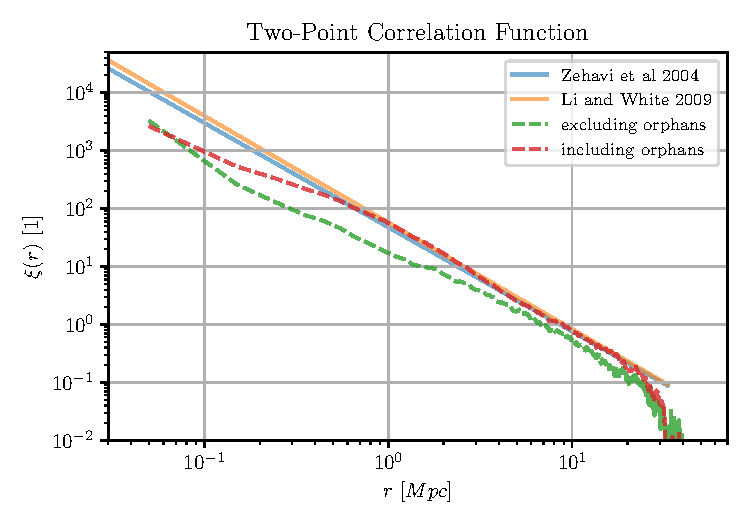
\includegraphics[width=\linewidth, keepaspectratio]{images/correlation.pdf}%
  \caption{The  predicted stellar  mass  2-point correlation  function
    (2PCF) $\xi(r)$ of our SHAM  model, including and excluding orphan
    galaxies, compared to  the power law fits of the  observed 2PCF in
    \citet{LiWhite} and \citet{Correlation1}.
  }%
  \label{fig:correlations}
\end{figure}

The  stellar mass  two-point correlation  function (2PCF)  $\xi(r)$ is
computed via  inverse Fourier transform  of the power  spectrum $P(k)$
\citep[e.g.][]{Mo},  which itself  can  be obtained  from the  Fourier
transform    of   the    stellar   mass    density   contrast    field
$\delta(\mathbf{r})$:
%
\begin{align}
  \delta_\mathbf{k} = \frac{1}{V}\int e^{i\mathbf{kr}} \delta(\mathbf{r}) \de ^3 \mathbf{r}
\end{align}
%
with
%
\begin{align}
	\delta(\mathbf{r}) = \frac{\rho(\mathbf{r})}{\langle \rho(\mathbf{r}) \rangle } - 1
\end{align}
%
Where $\rho(\mathbf{r})$ is the galaxy  stellar mass density field and
$\langle \rho(\mathbf{r}) \rangle$ is  the corresponding mean density,
$V = L^3$ is the volume of our large box on which the density field is
assumed  periodic,  and  $\mathbf{k}=\frac{2\pi}{L}(i_x,  i_y,  i_z)$,
where  $i_x,  i_y,  i_z$  are  integers.   The  Fourier  transform  is
performed using  the FFTW library \citep{FFTW05}.   The power spectrum
$P(k)$ and the 2PCF $\xi(r)$ are given by
%
\begin{align}
  P(k)    &= V \langle |\delta_\mathbf{k}|^2 \rangle \\
  \xi(r)  &= \frac{1}{(2\pi)^3} \int e^{-i\mathbf{kr}} P(k) \de^3 \mathbf{k} 
\end{align}
The simulation box is divided in  a uniform grid of $1024^3$ cells and
the  stellar mass  is  deposited  on the  grid  using a  cloud-in-cell
interpolation scheme.  The cloud-in-cell scheme consists  of assigning
each  galaxy a  cubic  volume  (``cloud'') the  size  of  a grid  cell
centered on the galaxy's position.  The galaxy stellar mass is assumed
to be uniformly distributed within the  cloud, and is deposited on the
uniform grid cells according to the  volume fraction of the cloud that
resides within each cell.

We only  include galaxies with  masses above $10^9 \msol$.   Using our
adopted SMHM relation,  these galaxies are hosted in  haloes with mass
larger than  $\sim 10^{11} \msol$,  or more than 300  particles.  This
threshold  ensures that  we  only  use well  resolved  clumps for  our
analysis, as discussed in the previous sections.

The predicted 2PCF $\xi(r)$ is shown in Figure \ref{fig:correlations},
and is  compared to  the observational  results of  \cite{LiWhite} and
\cite{Correlation1}.   Note  that  the observed  galaxy  catalogue  is
presented as  complete down  to $10^8 \msol$,  one order  of magnitude
smaller than our  simulated catalogue.  To highlight  the influence of
orphan galaxies,  we have  computed the predicted  2PCF both  with and
without  orphan  galaxies.   Including   orphan  galaxies  produces  a
correlation function in much  better agreement with observations.  Our
theoretical 2PCF obtained  reproduces the observed power  law fit over
two orders  of magnitude  in scale  of $r\sim 0.3  - 25$~Mpc.   On the
smallest  scales, below  0.3~Mpc,  our predictions  are  likely to  be
affected by our limited mass resolution and the grid resolution which 
is used for the Fourier Transform ($\sim 0.1$~Mpc per cell). We have 
verified that using a lower mass threshold for the stellar masses of 
galaxies makes no visible difference in the resulting correlation function.

The  role  of  the  orphan   galaxies  is  particularly  important  on
intermediate scales $\sim  0.2$ Mpc $<\ r \ <  2$ Mpc.  This behaviour
is explained by the fact that  orphan galaxies are located within host
haloes, thus contributing to the  correlations at small distances, the
so-called 1-halo term.  Our conclusion are in agreement  with those of
\cite{crisis}, who  have found that  the inclusion of  orphan galaxies
for mass-based SHAM models improves  the clustering statistics of mock
galaxy catalogues, particularly so at small scales.

%============================================================================
\subsection{Radial Profiles of Satellites in Large Clusters}\label{chap:radial-profiles}
%============================================================================

\begin{figure}
  \centering
  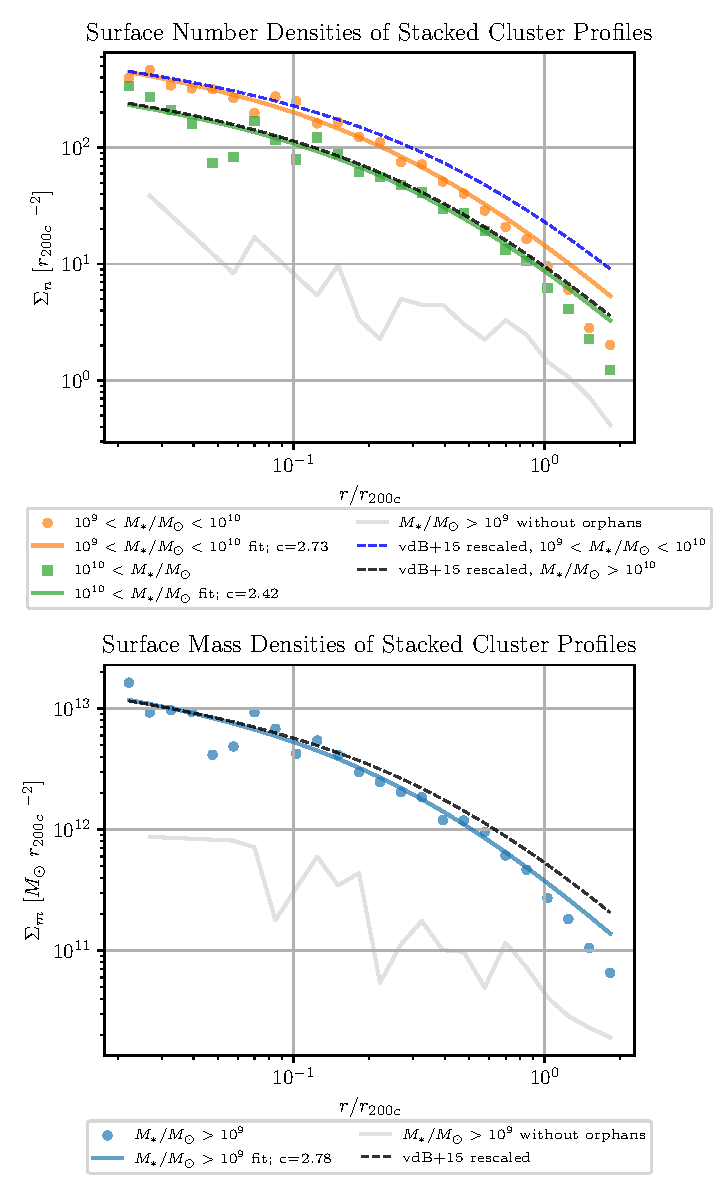
\includegraphics[width=\linewidth, keepaspectratio]{images/radial-profiles.pdf}%
  \caption{Upper panel: the light grey  solid line shows the satellite
    number density profile averaged over  the 10 largest haloes in our
    simulation {\it including only  satellite galaxies with a detected
    parent clump with masses above $10^9 \msol$}.   Satellites are  
    then grouped  in two  mass bins
    indicated in  the legend.   The colored  symbols show  the average
    number  density  profile  {\it  including  also  orphan  satellite
      galaxies}.  The colored solid  lines show the corresponding best
    fit projected NFW  profiles, while the  dashed lines  show the best  
    fit projected NFW profiles of the observed sample in
    \citet{vanderburgEvidenceInsideoutGrowth2015}.  Note  that for the
    latter,  we have  renormalized the  surface density  to match  the
    lower median mass of the  simulated sample (see text for details).
    The lower  panel shows the  stellar mass surface  density averaged
    over our  simulated sample. Here  again the light grey  solid line
    shows the  mass density profile  {\it only for  satellite galaxies
      within a detected  clump} while the blue symbols  shows the same
    quantity {\it also including  orphan satellite galaxies}. The blue
    solid  line corresponds  to our  best  fit projected NFW  profile while  the
    dashed line shows the best fit NFW profiles of the observed sample
    in \citet{vanderburgEvidenceInsideoutGrowth2015}.  Here again this
    last profile has  been renormalized to account  for the difference
    in  median mass  between the  simulated and  the observed  cluster
    samples.}
%
  \label{fig:radial-profiles}
\end{figure}

In this  section, we compute  the radial  profiles of number  and mass
densities  of satellite  galaxies in  the 10  largest clusters  in our
simulation. In  order to  compare to observations,  we will  follow as
closely      as     possible      the     method      described     in
\citet{vanderburgEvidenceInsideoutGrowth2015}, who analyzed 60 massive
clusters between 0.04<$z$<0.26 in  the Multi-Epoch Nearby Cluster Survey
and the Canadian Cluster Comparison Project.

We identified 10  haloes at $z=0$ with the highest  mass.  The mass is
defined here like  in \citet{vanderburgEvidenceInsideoutGrowth2015} as
$M_{200c}$, the  mass included within  radius $R_{200c}$ at  which the
average  enclosed  mass   density  of  the  halo  is   200  times  the
cosmological critical density $\rho_c$.   The $M_{200c}$ masses of our
10 selected  haloes range between  $1.4 \times 10^{14}\msol$  and $4.8
\times 10^{14}\msol$ with a median value of $1.6 \times 10^{14}\msol$.
Due to our limited box size, these  haloes are on the lower end of the
sample observed  in \citet{vanderburgEvidenceInsideoutGrowth2015}, who
reported masses ranging from $0.8 \times 10^{14}\msol$ and $1.6 \times
10^{15}\msol$ with a median value of $8.6 \times 10^{14}\msol$.

We compute  the projected number  density profiles and  projected mass
density  profiles as  follows: For  each  halo, we  first project  the
galaxies  (excluding the  central galaxy)  along each  coordinate axis
obtaining three  images.  We  then compute cylindrical  profiles using
radial shells equally space in log  radius in units of $r_{200c}$.  We
then average  the 30 profiles  (three projections for 10 clusters) to
obtain the final average radial surface density profile.  Each profile
is then fitted to a projected NFW profile \citep{navarroStructureColdDark1996b} using a
standard least square fitting procedure.   We obtain in particular the
concentration parameter that we can compare to the observed value.

The resulting profiles  are shown in Figure~\ref{fig:radial-profiles},
again including  and excluding  orphan galaxies. Orphan  galaxies play
here  also   a  crucial   role,  as   the  profiles   without  orphans
underestimate  the true  value by  an order  of magnitude.   Following
\citet{vanderburgEvidenceInsideoutGrowth2015},   we  adapt   the  same
galaxy  stellar   mass  $M_*$  thresholds   of  $10^9\msol  <   M_*  <
10^{10}\msol$ and $M_* > 10^{10}\msol$  for the surface number density
profile, and  a stellar mass threshold  of $M_* > 10^9  \msol$ for the
surface mass  density profile. It  is worth stressing that  this lower
mass threshold correspond exactly to  the mass resolution limit of our
mock galaxy catalogue.

As already noted above, the median  mass of the simulated and observed
catalogues  widely  differ.  In   order  to  facilitate  a  meaningful
comparison,  we  assume that  the  total  stellar mass  in  satellites
roughly  scales with  $M_{200c}$ in  the halo  mass range  of interest
here. We then adopt the following simple scaling relation
\begin{equation}
\Sigma \propto \frac{M_{200c}}{R_{200c}^2} \propto M_{200c}^{1/3}
\end{equation}
and    rescale    the    observed    average    profile    found    by
\citet{vanderburgEvidenceInsideoutGrowth2015}   using   this   scaling
relation  and  the  ratio  of  the  two  median  masses.  We  plot  in
Figure~\ref{fig:radial-profiles} the corresponding best fit projected NFW
profiles, showing excellent agreement with our simulated results.

Interestingly, the  observed surface density profiles  have a slightly
smaller concentration than  the simulated ones.  Although  we find for
the  number densities  of  satellite galaxies  above $10^{10}\msol$  a
concentration $c  = 2.4$,  in strikingly  good agreement  with $c=2.3$
found  by \citet{vanderburgEvidenceInsideoutGrowth2015}  for the  same
mass range, our results differ for the  mass range $10^9 \msol < M_* <
10^{10}        \msol$:       we        find       $c=2.7$        while
\citet{vanderburgEvidenceInsideoutGrowth2015} found  $c=1.8$. The same
mismatch is  found using the  mass density profile.  we  find $c=2.8$,
while \citet{vanderburgEvidenceInsideoutGrowth2015} found $c=2.0$.

We  believe  that this  mismatch  in  the concentration  parameter  is
consistent  with  the   difference  we  have  in   the  median  sample
mass. Indeed, the  theory predicts a larger  concentration for smaller
mass haloes, roughly in the amplitude observed here \citep{zhaoAccurateUniversalModels2009}. 
We therefore  could in principle improve the agreement
between   our    simulation   results   and   the    observations   of
\citet{vanderburgEvidenceInsideoutGrowth2015}  by  also rescaling  the
radial direction according to the theoretical expectations. We believe
this is  beyond the  scope of this  paper to try  and fit  exactly the
data.

In   addition,    we   believe   there    is   much   more    to   the
story. \citet{vanderburgEvidenceInsideoutGrowth2015} found that larger
mass  satellite galaxies  have  a  significantly larger  concentration
parameter   than    the   low   mass   bin    ($c=2.3$   compared   to
$c=1.8$). Moreover, they have also  found a strong excess of satellite
galaxies compared to the best fit NFW  profile in the centre ($r < 0.1
R_{200c}$).   These observations  are  consistent with  the effect  of
dynamical friction  bringing the more  massive galaxies faster  to the
central regions of  the cluster. Dynamical friction is  expected to be
sufficiently efficient  for the  most massive  sub-haloes, with  a mass
larger than a few  percent of that of the host  halos 
\citep[e.g.][]{binneyGalacticDynamicsSecond2008,Mo}. 
In our case, this  translates into
sub-haloes  more  massive  than  a  few  $10^{12}\msol$  and  satellite
galaxies  more  massive than  a  few  $10^{10}\msol$.  Our  simulation
clearly suffers from  numerical overmerging in this  mass range 
\citep{vandenboschDisruptionDarkMatter2018}, as highlighted  by the 
importance of including  orphan galaxies in
our  methodology.  Moreover,  our  pure DMO  parent simulation  cannot
follow precisely the many baryonic  effects that are needed to predict
accurately the  individual trajectory  of these higher  mass satellite
galaxies.

With these  caveats in mind,  we conclude  that using our  merger tree
code and a  state-of-the-art SHAM method, we can  model reasonably well
the cluster satellite galaxy number density and mass density profiles.

    %=================================================
\section{Conclusion}\label{chap:conclusion}
%=================================================




An algorithm to identify dark matter halo merger trees, designed to work on the fly on parallel computing systems with the adaptive mesh refinement code \ramses, was presented.
Clumps of dark matter are tracked across snapshots through up to some user-defined number, $n_{mb}$, of particles they consist of.
The best choice for $n_{mb}$ seems to be around 100-200, where the trade-off between computational cost and performance appears optimal.
Furthermore, the influence of various definitions of substructure properties on the resulting merger tree were tested.
Whether substructures contain their respective substructures' masses or not had negligible effect on the merger trees.
However defining particles of substructure to be gravitationally bound to that substructure if and only if the particles can't leave the spatial boundaries of that substructure leads to much less extreme mass growths and extreme mass growth fluctuations of dark matter clumps, suggesting that it should be the preferred definition for accurate merger trees.

In agreement with the bottoms-up hierarchical structure formation picture for dark matter haloes, the merger trees of massive haloes at $z=0$ were found to tend to have more branches and their formation history can often be traced to very high redshifts.
Even clumps on the lower mass end were successfully tracked back to high redshifts.


With the known formation history of dark matter clumps, using a stellar-mass-halo-mass relation (eqns. \eqref{eq:SMHM_start}-\eqref{eq:SMHM_end}) galaxies can be placed in a dark matter only simulation to obtain mock galaxy catalogues.
The galaxies are placed at the position of the most tightly bound particle of any dark matter clump.
Once a clump merges into another and dissolves beyond the possibility of identification, its last assigned galaxy is kept track of.
Such an ``orphan'' galaxy is used two reasons.
Firstly, just because a clump can't be identified any more due to the environment it currently resides in, it doesn't mean that the galaxy that it hosted is also dissipated.
On the contrary: \cite{Nagai} showed that tidal stripping of galaxies inside a dark matter halo sets in much later than for the subhalo they reside in.
Secondly, it is possible for a subhalo to re-emerge from its host halo at later snapshots because it wasn't detected by the clump finder in the density field of the host halo, but still existed.
Such a situation is illustrated in figure \ref{fig:jumper-demo}.
In these cases, orphan galaxies are used to establish a link between progenitor and descendant clumps across multiple snapshots.

However, the current implementation only contains the option to forget past merged progenitors after a user defined number of snapshots has passed, but by default, it will track them until the simulation ends.
This might lead to misidentifications of progenitor-descendant pairs and therefore wrong formation histories.
Solutions for this problem would be either to remove the orphans after the estimated time for them to merge into the parent structure has passed, which could be e.g. the dynamical friction time (eq. \eqref{eq:dynamical_friction_time}), or introduce some form of galaxy-galaxy merging cross sections to compute the probability of a collision between galaxies that will result in a galaxy merger.

From a technical viewpoint, one clear bottleneck in the current merger tree algorithm is the requirement to write progenitor particles and data to file and read them back in and sort them out at a later snapshot. 
A possible improvement would be to track which particles left each task’s domain and which particles entered in between two snapshots. The progenitor particles would still be read and written to and from files, but it would minimise the sorting part of the algorithm where each MPI task figures out which tracker particles it contains.
Another option would be to change the amount of data each MPI task needs to read in. 
The maximal velocity of any particle in the time interval between two snapshots should be traced. This way, once the simulation advances to the next snapshot, it would be possible to estimate the maximal distance any particle could’ve travelled.
Provided every MPI task has knowledge on how the entire computational domain is split between tasks, it could skip reading in data written by tasks where no particle currently in this task’s domain could have come from.



Given that the mock galaxy catalogues in this work were created using simulations with relatively low spatial and mass resolution of $512^3$ particles in boxes of 69 and 100 comoving Mpc each, the obtained correlation functions (shown in figure \ref{fig:correlations}) and stellar mass functions (figure \ref{fig:smf}) show good agreement with observed stellar mass functions.
By comparing the results of the two simulations it can be expected that a higher spatial resolution should improve the clustering statistics, and together with a higher mass resolution the stellar mass functions of central galaxies should also improve.





       
       
       
       
       
%%%%%%%%%%%%%%%%%%%%%%%%%%%%%%%%%%%%%%%%%%%%%%%%%%

%%%%%%%%%%%%%%%%%%%% REFERENCES %%%%%%%%%%%%%%%%%%

    % The best way to enter references is to use BibTeX:
    
    \bibliographystyle{mnras}
    \bibliography{references} % if your bibtex file is called references.bib
    
    \appendix
   	%========================================================================================================
\section{Tree Statistics Using \citet{SUSSING_HALOFINDER} Selection Criteria}\label{app:performance_comparison}
%========================================================================================================



\begin{table}
\centering
\caption{
	Comparison of simulation and evaluation parameters used in this work and of A14, where the parameters of the latter have been converted using $h = 0.704$.
	$m_m$ is the mass threshold for main haloes, $m_s$ is the mass threshold for sub-haloes.
	\label{tab:parameter-comparison}
}
	\begin{tabular}[c]{l l l}
																	&	This work		&	A14 \\
		\hline
		particle mass	[$10^9 \msol$]	&	$1.55$			& $1.32$						\\
		particles used								& $256^3$			& $270^3$ 					\\
		box size [Mpc/h]							& $62.5$			& $62.5$						\\
		snapshots until $z = 0$				& 62					& 62								\\				
		$m_m$ [$10^{12} \msol$]				&	$1.35$			& $1.12$ - $1.37$		\\
		$m_s$ [$10^{11} \msol$]				&	$4.03$			& $4.26$ - $9.72$		\\
		\hline
	\end{tabular}
\end{table}


\begin{figure}
	\centering
	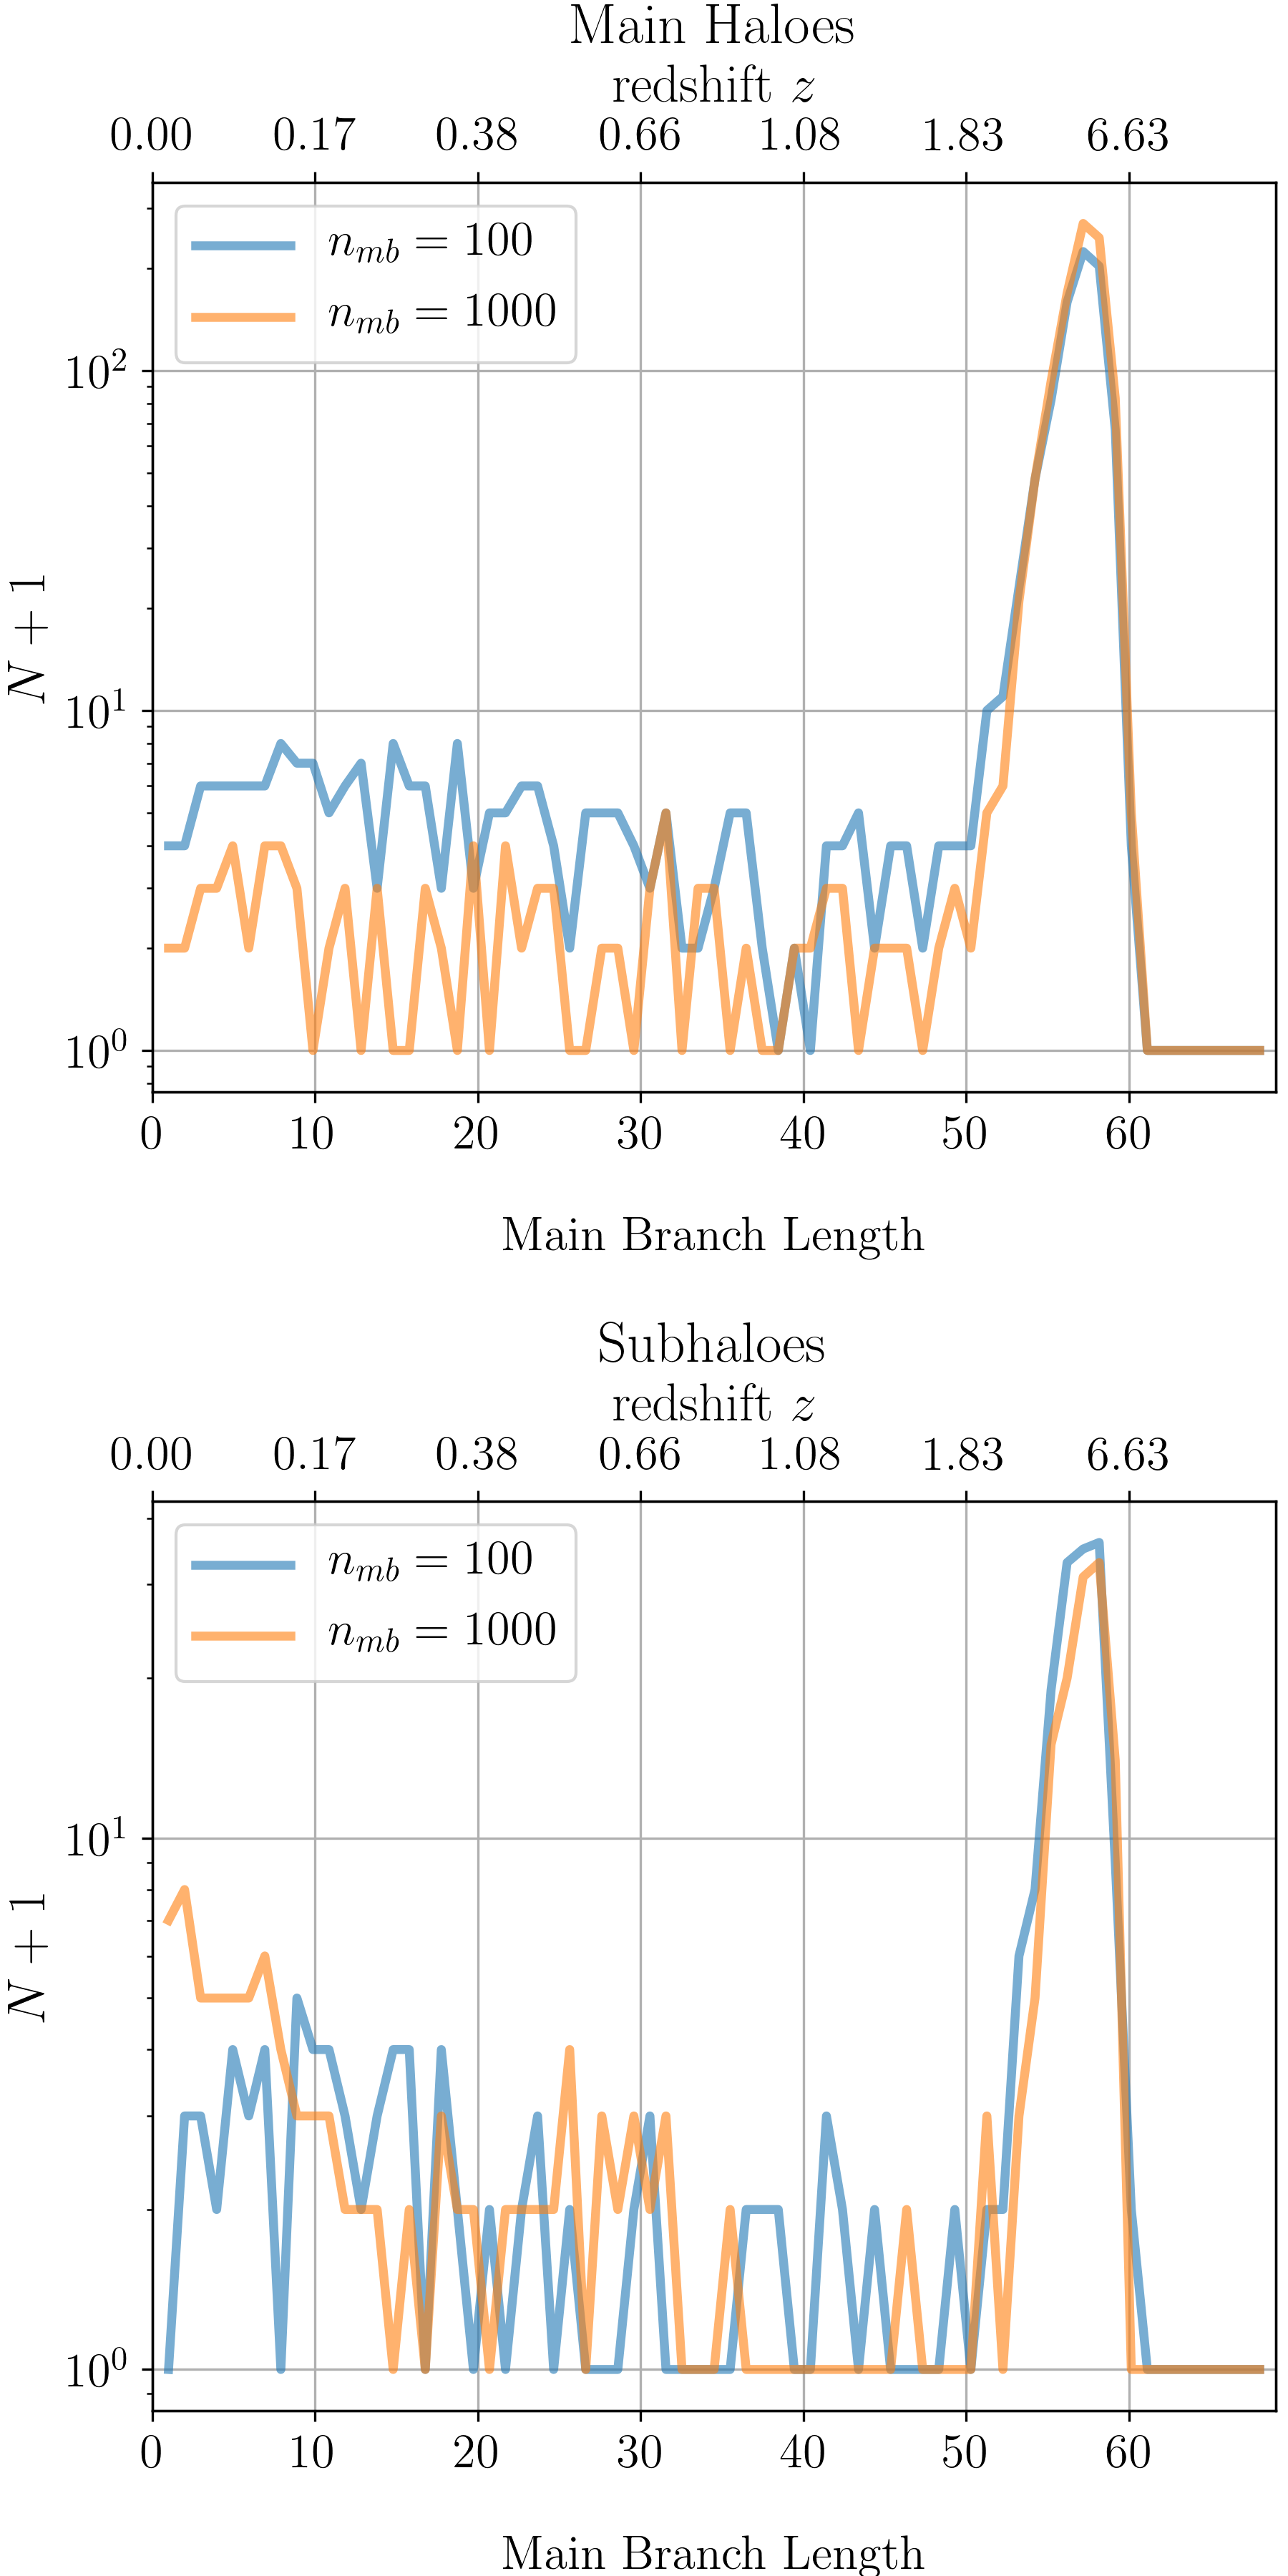
\includegraphics[width=.95\linewidth, 
	keepaspectratio]{images/tree-statistics-sussing-threshold/main-branch-lenghts-all-bins-ntrace.png}%
	\caption{
		Histograms of the length of the main branch. 
		The top plot shows the length of the 1000 most massive haloes at $z = 0$, the bottom plot shows 
		the length of the 200 most massive sub-haloes for $n_{mb} = 100$ and $1000$ tracer particles 
		per clump.
	}%
	\label{fig:sussing-branch-lengths}
\end{figure}


\begin{figure}
	\centering
	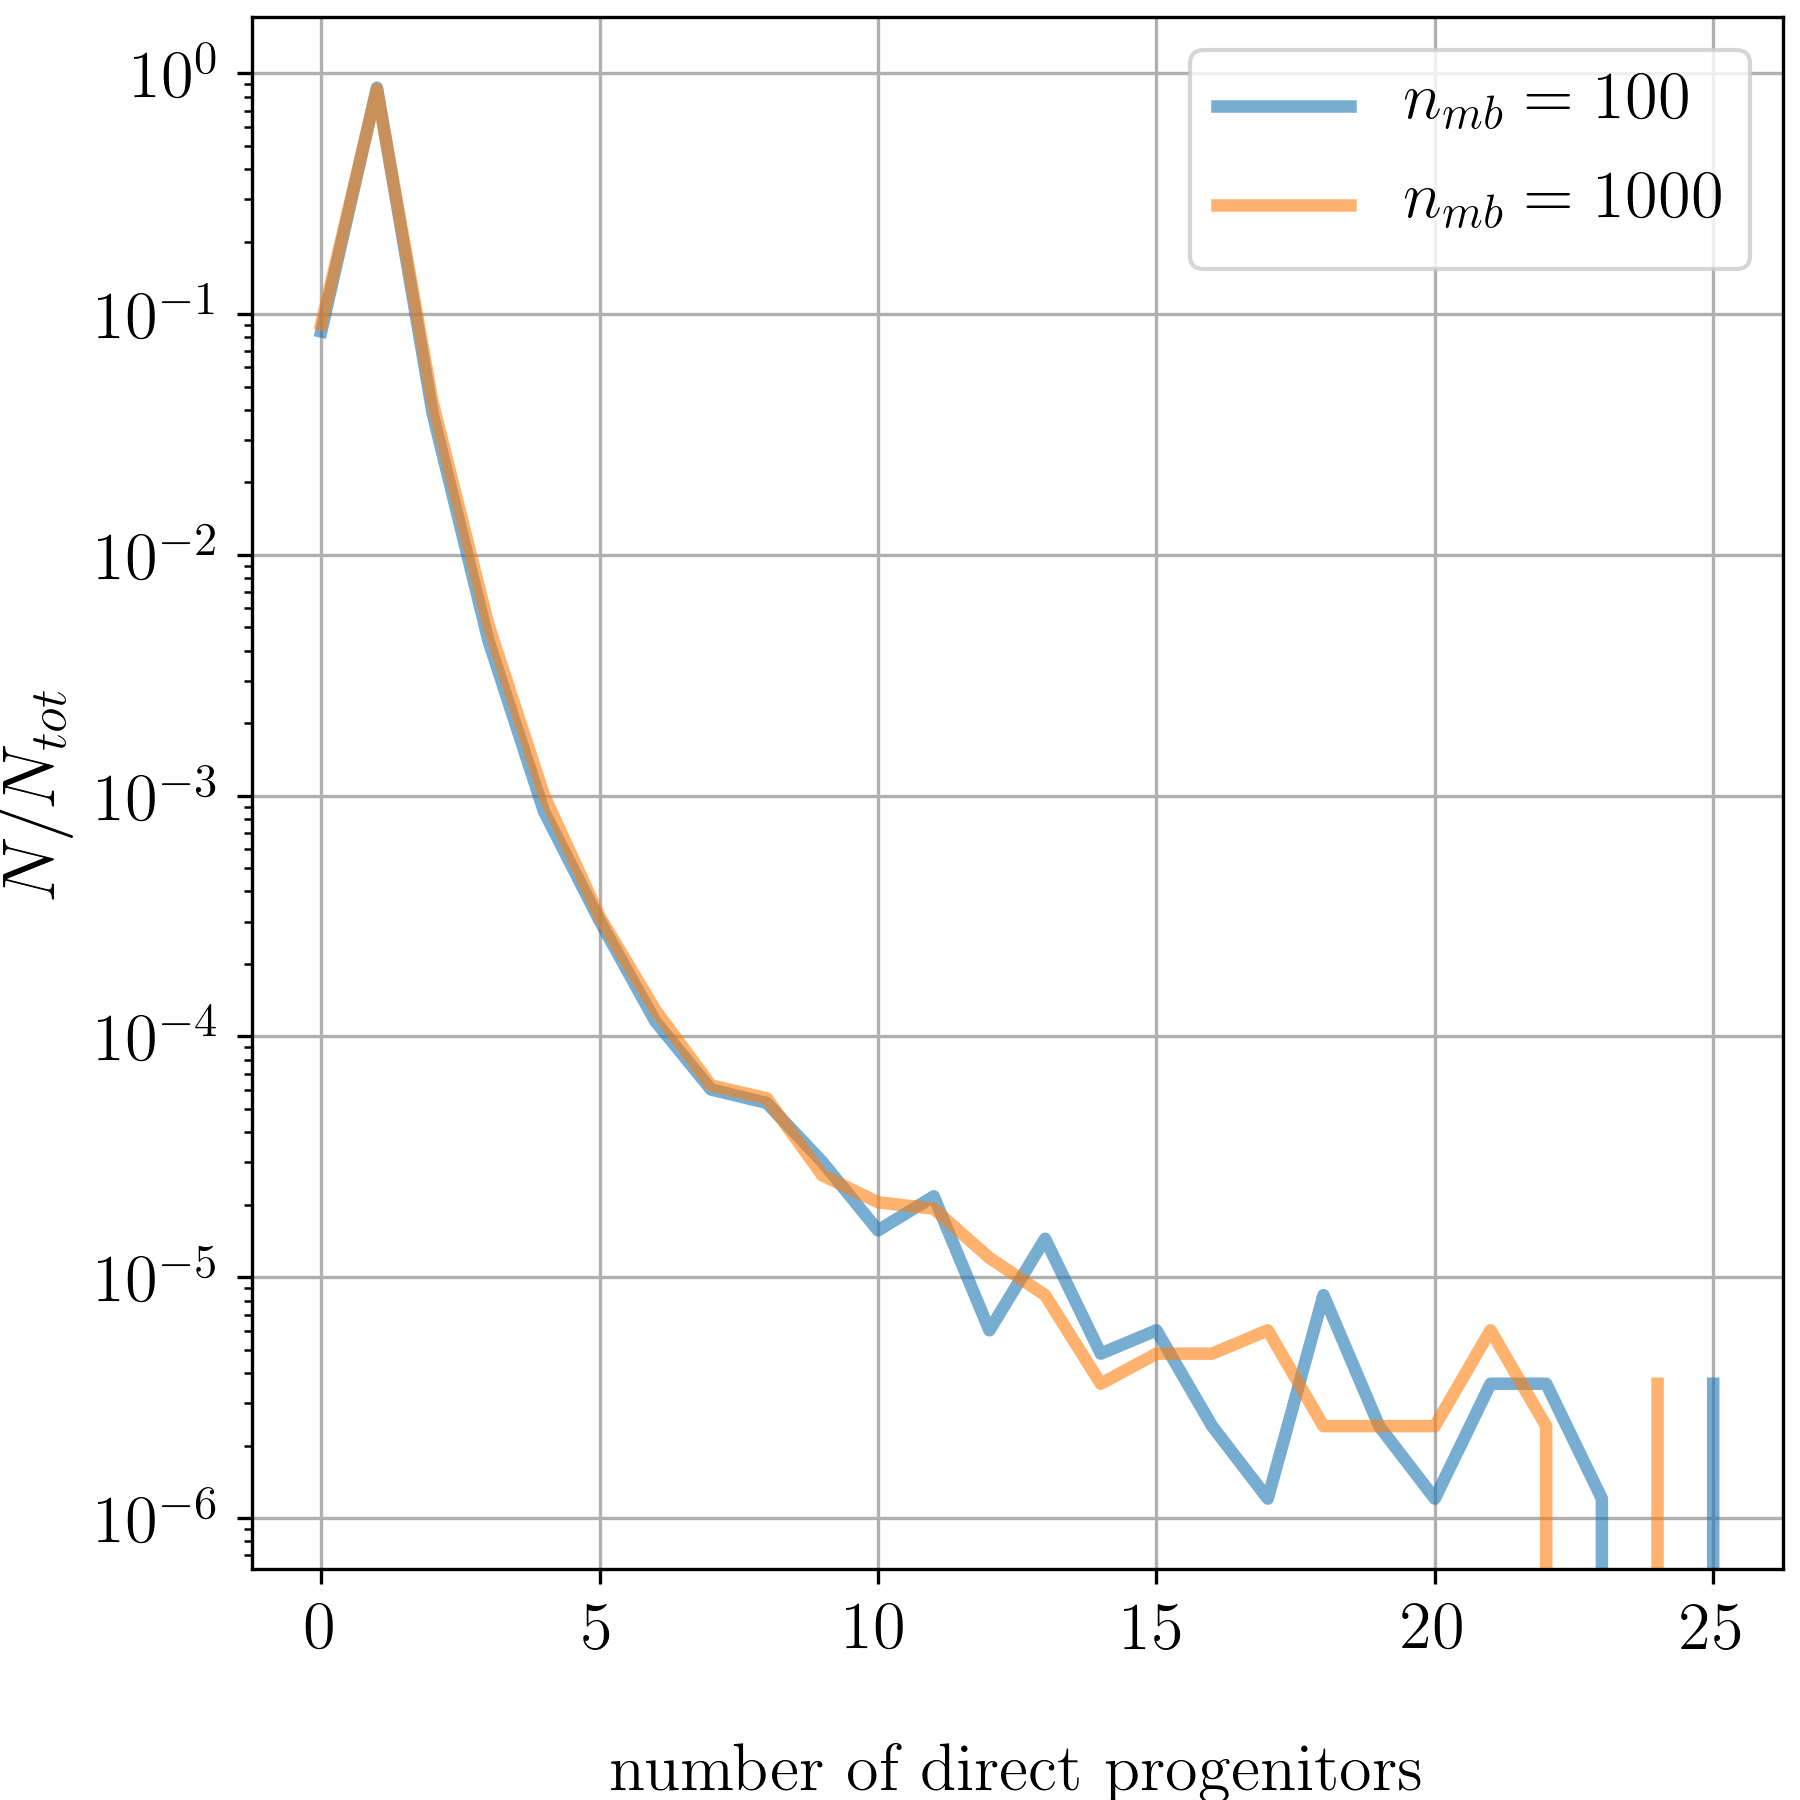
\includegraphics[width=.9\linewidth, keepaspectratio]{images/tree-statistics-sussing-threshold/branching-ratio-ntrace.png}\\%
	\caption{
		Histogram of the number of direct progenitors for all clumps from $z = 0$ to $z = 2$ for $n_{mb} = 100$ and $1000$ tracer particles per clump.
		The histogram is normalized by the total number of events found.
	}%
	\label{fig:sussing-branching-ratio}
\end{figure}


\begin{figure*}
	\centering
	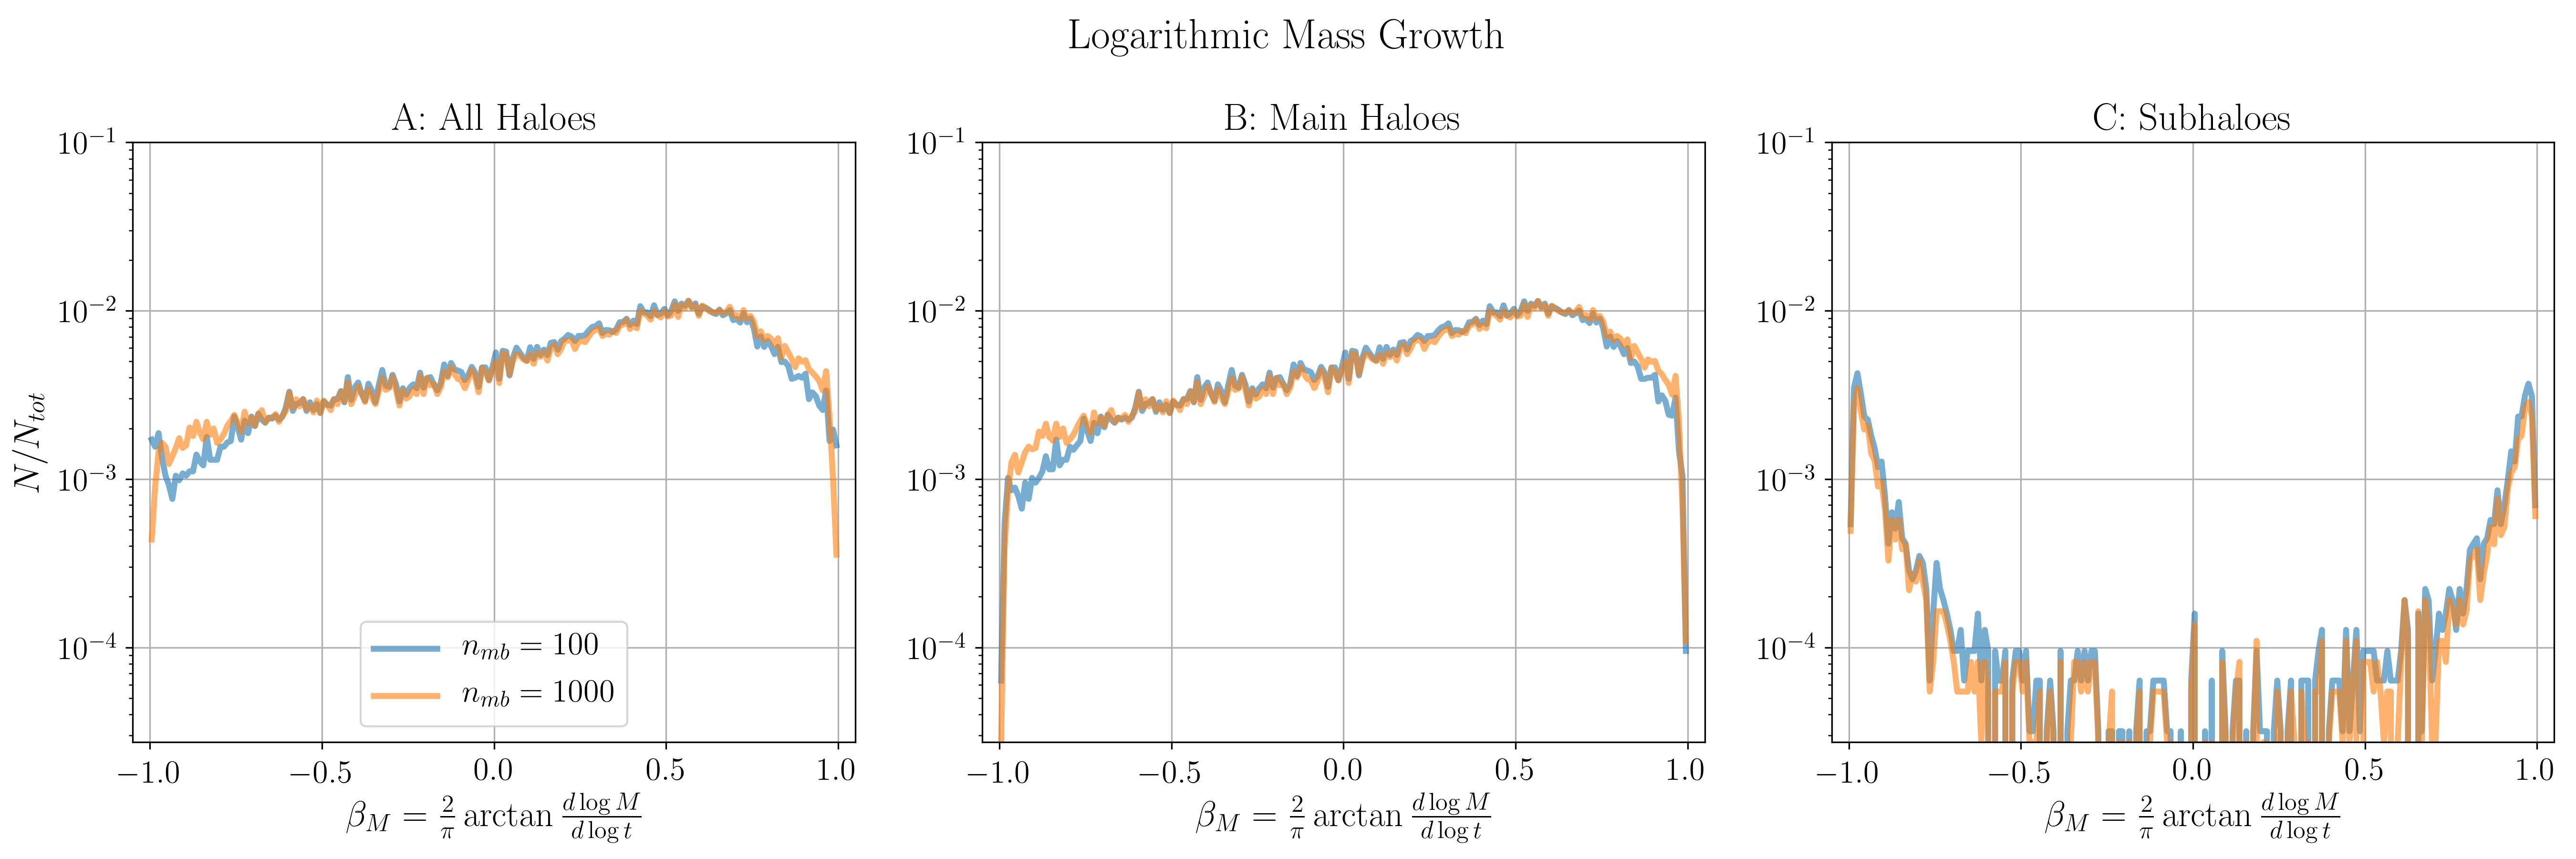
\includegraphics[width=\textwidth, keepaspectratio]{images/tree-statistics-sussing-threshold/mass_growth-ntrace.png}%
	\caption{
		Logarithmic mass growth for haloes and sub-haloes satisfying the mass thresholds.
		Group $A$ contains clumps that are either haloes or sub-haloes in consecutive snapshots $k$ and $k+1$ with masses $m \geq m_{m}$.
		Group $B$ contains clumps that are only haloes in two consecutive snapshots with mass above $m_{m}$, group $C$ contains only clumps that were sub-haloes in two consecutive snapshots with mass greater than $m_{s}$.
		The histogram is normalized by the total number of events found for group $A$.
	}%
	\label{fig:sussing-mass-growth}
\end{figure*}

\begin{figure*}
	\centering
	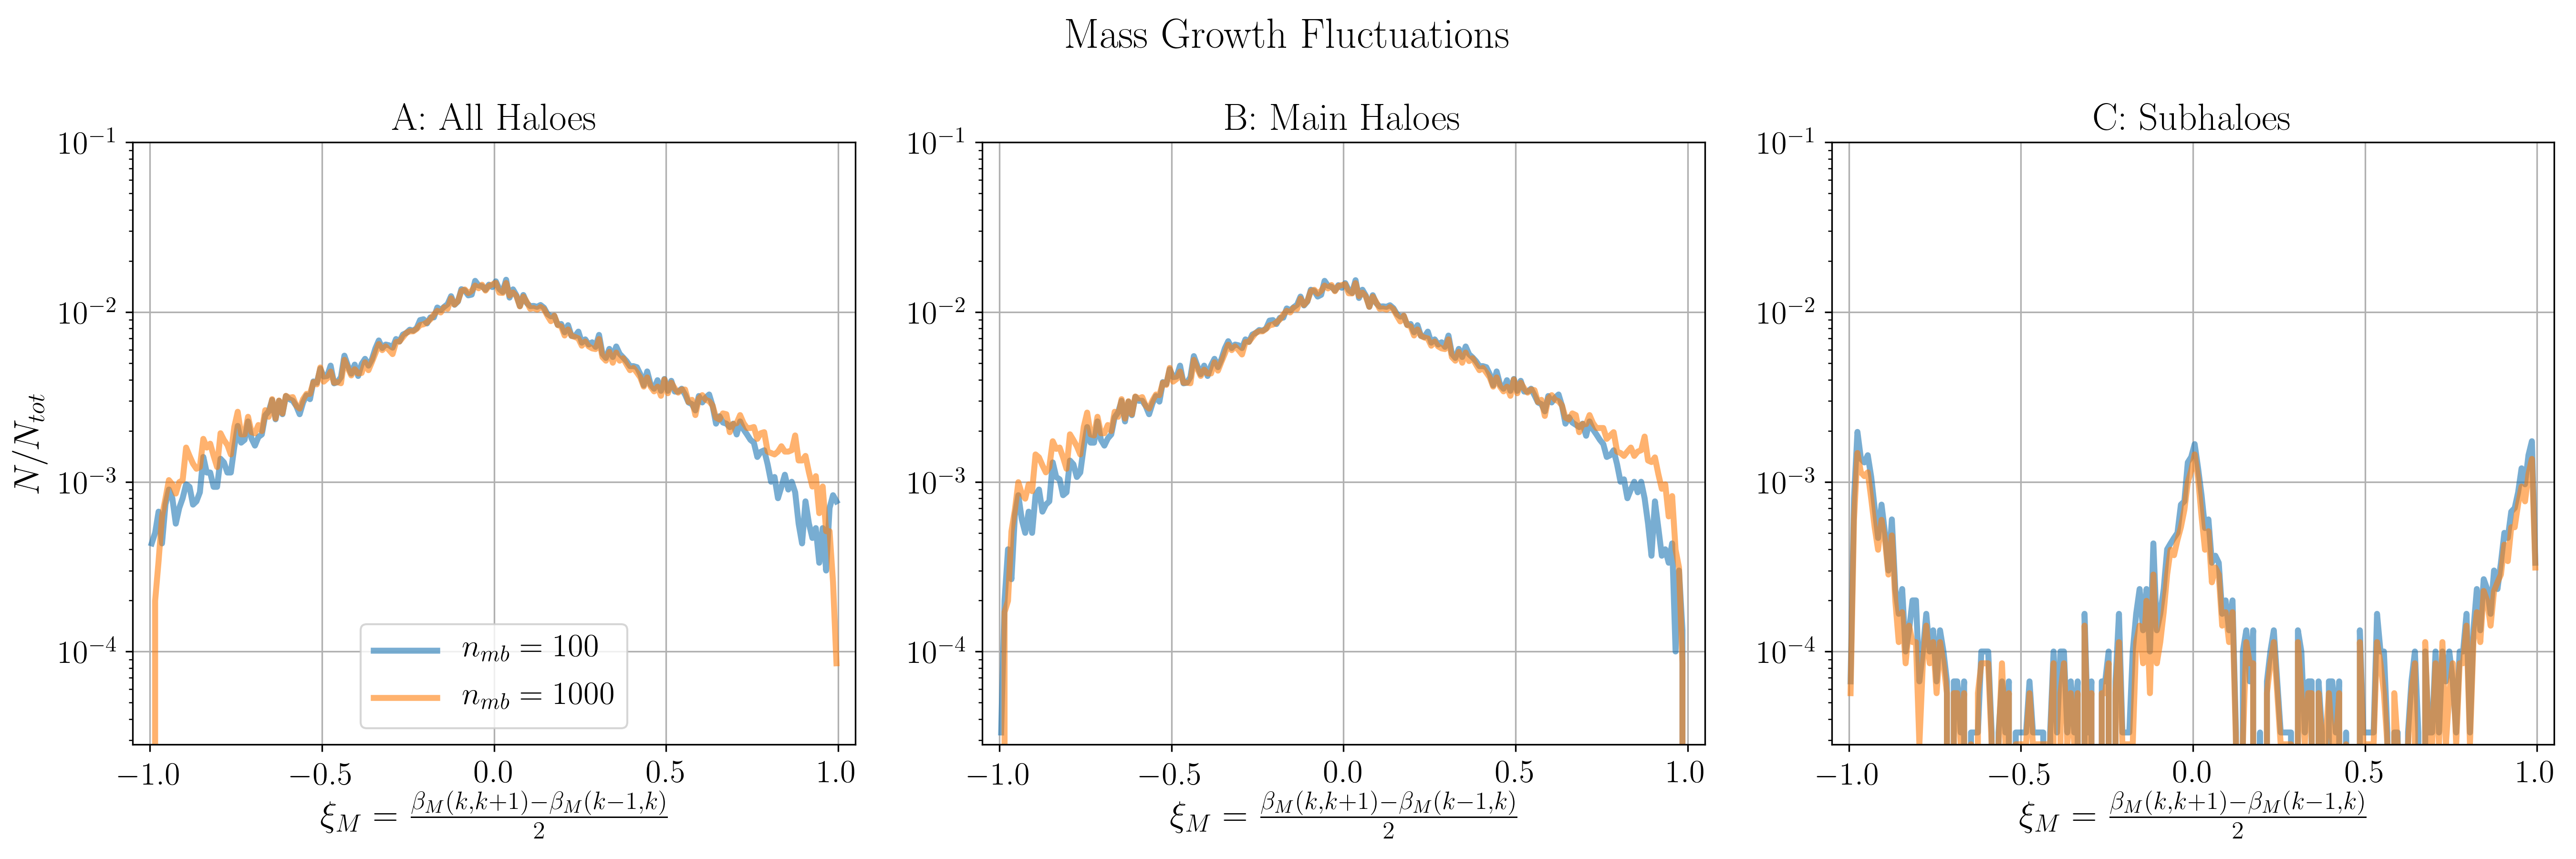
\includegraphics[width=\textwidth, keepaspectratio]{images/tree-statistics-sussing-threshold/mass_fluctuations-ntrace.png}\\%
	\caption{
		Histogram of mass growth fluctuations for haloes and sub-haloes satisfying the mass thresholds.
		Group $A$ contains clumps that are either haloes or sub-haloes in three consecutive snapshots with masses $m \geq m_{m}$.
		Group $B$ contains clumps that are only haloes in three consecutive snapshots with mass above $m_{m}$, group $C$ contains only clumps that were sub-haloes in three consecutive snapshots with mass greater than $m_{s}$.
		The histogram is normalized by the total number of events found for group $A$.
	}%
	\label{fig:sussing-mass-fluct}
\end{figure*}




In this section, the merger tree statistics introduced in Section \ref{chap:tests} when following the selection criteria that are used in \citet{SUSSING_HALOFINDER} (A14 from here on) are presented.
Ideally, \texttt{ACACIA} should be tested on the same datasets and halo catalogues used in the Comparison Project to enable a direct comparison to the performance of other merger tree codes. 
However, since \texttt{ACACIA} was designed to work on the fly, using it as a post-processing utility would defeat its purpose.
Furthermore, \texttt{ACACIA} is not necessarily compatible with other definitions of haloes and sub-haloes.
But most importantly, we also want to demonstrate that the halo finder \phew\ can be used to produce reliable merger trees. 
So instead, the tests are performed on our own datasets and halo catalogues, which are described in section \ref{chap:testing_methods}.
A comparison of the used parameters of our simulations and the ones used in A14 is given in Table \ref{tab:parameter-comparison}.
In the following, the results for $n_{mb} = 100$ and $n_{mb} = 1000$ are shown.
Like before, when the influence of the number of tracer particles was investigated, the \sad\ parameter and the \exc\ mass definition were used.


The difference to the results presented in Section \ref{chap:tests} is that the mass thresholds are set such that only the 1000 most massive main haloes and only the 200 most massive sub-haloes at $z = 0$ are included.
This gives effective mass threshold $m_{m} = 1.35 \times 10^{12} \msol$ and $m_{s} = 4.0 \times 
10^{11}\msol$, which are on one hand comparable to the mass thresholds applied in A14 (Table 
\ref{tab:parameter-comparison}), but already show differences in the resulting halo catalogue.
\phew\ finds a mass threshold for main haloes that is close to the upper limit found in A13, 
but a lower mass threshold for sub-haloes.
This is consistent with the fact that the \sad\ parameter was used:
Unbound particles are passed on to substructure that is higher up in the hierarchy, and the unbinding is repeated until the top level, which are the main haloes, is reached.
The more strict unbinding criterion tends to assign more particles to the main haloes and remove them from sub-haloes, which is reflected in the mass thresholds.
Indeed, using the \nosad\ parameter instead leads to $m_m = 1.27 \times 10^{12}\msol$ and $m_s = 
1.92 \times 10^{12}\msol$.



The length of the main branches for haloes and sub-haloes individually are shown in Figure 
\ref{fig:sussing-branch-lengths}. Compared to Figure 3 of A14, we note the following similarities 
and differences:
%
\begin{enumerate}
	\item \texttt{ACACIA} finds some main haloes with short (< 10) main branches.
		In A14, his only happens for the \texttt{JMerge} and \texttt{TreeMaker} tree builders
		regardless	of the halo finder employed, and the \texttt{MergerTree}, \texttt{SubLink}, 
		and \texttt{VELOCIraptor} tree makers for \texttt{AHF} and \texttt{Subfind} halo finders.
%	
	\item Like in nearly all cases in A14, the distribution of main branch lengths for
		main haloes peaks at high numbers and the bulk of the distribution is about 20 snapshots
		wide. The peak of the main branch length distribution of \texttt{ACACIA} is at 40,
		while in most cases in A14, it's around 45 with the exception of the \texttt{AHF}
		halo finder. This indicates that \texttt{ACACIA} and \phew\ result in on average 
		somewhat smaller main branch lengths than other codes. However, we also find the 
		maximal main branch length of 50, while nearly all combinations of
		halo finders and tree makers in A14 find higher values. Both these differences can be 
		explained by the slightly lower resolution that we used in our simulations, where we 
		found no identifiable clumps before snapshot 11, which corresponds to a maximal main 
		branch length of 51. 
%
	\item The main branch lengths for sub-haloes also follow the trends noted above. Additionally,
		the distribution is flat for main branch lengths smaller than 30, which is not the case
		for \texttt{Rockstar} and \texttt{AHF} sub-haloes in A14 for nearly all tree builders. Instead,
		their main branch lengths peak again around unity.
\end{enumerate}
%
In summary, regarding the main branch lengths of main haloes, \phew\ and \texttt{ACACIA} perform
comparably to \texttt{Subfind} and \texttt{Rockstar} halo finders and \texttt{MergerTree}, 
\texttt{TreeMaker}, and \texttt{VELOCIraptor} tree builders. Concerning sub-haloes, the results are
most closely to \texttt{Subfind} sub-haloes and the same tree builders as for the main haloes. This 
is not surprising, because \texttt{Subfind} employs a similar definition of substructure being 
arbitrarily shaped self-bound structure that is truncated at the isodensity contour that is 
defined by the density saddle point between the sub-halo and the main halo. 

In Figure \ref{fig:sussing-branching-ratio} the number of direct progenitors for all clumps between 
$z = 0$ and $z = 2$ are shown. Comparing to Figure 5 of A14, \texttt{ACACIA} gives very comparable 
results: $\sim 10^{-1}$ haloes have no direct progenitor, almost all have one, and the distribution 
follows an exponential decay with the maximal number of direct progenitors lying around 20-25, save 
for a very few outliers. Many tree makers and halo finders in A14 exhibit the same kind of 
behaviour, particularly so for the \texttt{AHF}, \texttt{Subfind}, and \texttt{Rockstar all} halo 
finders in Figure 5 of A14.


For the logarithmic mass growth (Figure \ref{fig:sussing-mass-growth}) and the mass growth fluctuations (Figure \ref{fig:sussing-mass-fluct}), the statistics are separated into three groups.
Group $A$ contains clumps that are either haloes or sub-haloes in \emph{consecutive} snapshots $k$ 
and $k+1$ with masses greater than the mass threshold $m_m$ in both snapshots. Group $B$ contains 
clumps that are exclusively main haloes in two consecutive snapshots with mass above $m_{m}$, group 
$C$ contains only clumps that were sub-haloes in two consecutive snapshots with mass greater than 
$m_{s}$. We follow clumps of the $z = 0$ snapshot along the main branch only.

The logarithmic mass growth resulting from \texttt{ACACIA} follows the general trend that the tree 
makers in A14 exhibit too. The growth for groups $A$ and $B$ increases steadily and peaks around 
$\beta_M \sim 0.5$, where the peak is $\sim2 \times 10^{-2}$. For $n_{mb} = 100$, the extreme mass 
loss  with $\beta_M = -1$ increases for group $A$, which is an undesirable property, but is also 
exhibited by \texttt{Sublink} in A14. For $n_{mb} = 1000$, it drops to about $10^{-3}$ ($10^{-4}$ 
for group $B$), which is comparable behaviour to \texttt{MergerTree}, \texttt{Sublink}, and 
\texttt{VELOCIraptor}, particularly so in combination with \texttt{AHF} and \texttt{Subfind} halo 
finders. Group $C$, containing only mass growths of clumps that have been sub-haloes in two 
consecutive snapshots, shows a distribution peaking around extreme mass growths $\beta_M 
\rightarrow \pm 1$ at $\sim 5 \times 10^{-3}$, which can again be seen in A14 for almost all tree 
makers, albeit not for all halo finders. More noticeably, almost no sub-haloes are found with $-0.5 
< \beta_M < 0.5$ with \phew\ and \texttt{ACACIA} in Figure \ref{fig:sussing-mass-growth}.
This is due to the fact that once a halo is merged into another, it quickly loses its 
outer mass due to the strict unbinding method used here. However, the distribution that 
\texttt{ACACIA} finds displays some differences with respect to the results in A14. Firstly,
we find almost no mass growth with $-0.5 < \beta_M < 0.5$, similar only to the results of 
\texttt{JMerge} in A14. This is partially due to the strict selection criteria used for this 
analysis: We only include clumps that are classified as sub-haloes in two consecutive snapshots and 
satisfy the mass threshold $m_s$ in both snapshots as well. In particular, this excludes all 
non-adjacent ``jumper'' links that we find, since we don't modify the halo catalogue like e.g. 
\texttt{ConsistentTrees}. Furthermore, we employ the \sad\ unbinding criterium, which strips more
particles from sub-haloes and assigns them to main haloes, leaving the halo catalogue with fewer 
sub-haloes that satisfy the mass threshold. When we instead use the \nosad\ 
criterium, we find that the distribution is on average around $3 \times 10^{-4}$ for $-0.5 < 
\beta_M < 0.5$, albeit noisy, which is in good agreement with most halo finders and tree builders 
in A14. 
Secondly, the distribution \texttt{ACACIA} finds looks remarkably symmetric w.r.t. $\beta_M = 0$.
While e.g. \texttt{MergerTree} and \texttt{TreeMaker} trees with \texttt{AHF}, \texttt{Subfind}, 
and \texttt{Rockstar} haloes find peaks close to $\beta \pm 1$ of similar height, they are also 
always have distributions skewed towards mass losses $\beta_M < 0$ and the peaks at $\beta_M = -1$ 
higher than the one at $\beta_M = 1$. 

We found that the reason why our distribution looks so 
symmetrical is due to the particle unbinding method and the way sub-halo hierarchies are 
established in \phew, similarly to what we have found to be a reason for the short main branch
lengths in Section~\ref{chap:varying_clump_mass_definition}. The hierarchy is determined by the 
density of the density peak of each clump: 
A clump with a lower peak density will be considered lower in the hierarchy of substructure. So in 
situations where two adjacent sub-haloes have similarly high density peaks, their order in the 
hierarchy might change in between two snapshots due to small changes. The unbinding algorithm then 
strips the particles from the sub-haloes that have the lowest level in the hierarchy and passes it 
on to the next level, amplifying the mass loss which these sub-haloes experience. If in the next 
snapshot the order in the hierarchy for these two clumps are inverted, the clump which experienced 
a mass loss previously will now experience a strong mass growth and vice versa. In 
Figure~\ref{fig:sussing-mass-growth} such an oscillation over two snapshots will simultaneously add 
a strong mass growth and a strong mass loss twice in place of a net smoother mass loss, leading to 
the symmetry of the distribution. We verified that about 10$\%$ of strong mass growth events with 
$\beta_M > 0.75$ are also accompanied by the respective sub-haloes increasing their level in the 
hierarchy. Similarly, about 10$\%$ of strong mass loss events with $\beta_M < -0.75$ are 
accompanied by the respective sub-haloes decreasing their level in the hierarchy.


The mass growth fluctuations (Figure \ref{fig:sussing-mass-fluct}) of \texttt{ACACIA} share the 
general trend with the ones from Figure 8 in A14, in that they peak around $\xi_M = 0$ and decrease 
outwards towards $\xi_M = \pm 1$. In A14, in all cases groups $A$ and $B$ peak just below 
$10^{-1}$, while our results peak around $4 \times 10^{-2}$. However, similarly to the results of 
e.g. \texttt{Sublink}, \texttt{TreeMaker}, and \texttt{VELOCIraptor} with the \texttt{AHF} or 
\texttt{Subfind} halo finders, the distribution around $\xi_M \sim \pm 0.5$ drops to $\sim 5 \times 
10^{-3}$, and then continues dropping below $10^{-4} - 10^{-3}$ at $\xi_M \sim \pm 1$. 
%For $n_{mb} = 100$, the group $A$ distribution rises again for $\xi_M \sim 1$, as it does for 
%\texttt{TreeMaker} and \texttt{Sublink} tree makers with \texttt{AHF}. 
Group $B$ shows a steeper drop around the extreme values $\xi_M \sim \pm 1$ compared to group $A$, 
dropping below $10^{-4}$ at these values, similarly to the behaviour of many tree makers and halo 
finders in A14.
The sub-halo group $C$ of this work shows three main peaks, around $-1$, $0$, and $1$.
These peaks also appear in the A14 results.
However, the peaks at the extreme values in A14 are lower than the ones of this work, while the 
peaks around $0$ is higher. The reason why these peaks are so pronounced in our results is the same 
as for why the mass growths in Figure~\ref{fig:sussing-mass-growth} is remarkably symmetric 
compared to others: it's sub-haloes and their respective sub-sub-haloes switching their order in the 
substructure hierarchy repeatedly and the particle unbinding algorithm stripping particles from the 
lower level substructure and assigning it to the higher level substructure.
The missing values around $\xi_M \sim \pm 0.5$ that were also seen in the mass growth in Figure 
\ref{fig:sussing-mass-growth} remain unsurprisingly, and are mitigated if the \nosad\ unbinding 
criterion is applied instead.
Similar distributions are obtained by e.g. the \texttt{AHF} and \texttt{Rockstar} halo finders in 
combination with the \texttt{MergerTree}, \texttt{JMerge}, \texttt{Sublink}, and \texttt{TreeMaker} 
tree builders.

In summary, we find that \texttt{ACACIA} and \texttt{PHEW} produce merger tree statistics which are 
similar to what multiple other state-of-the-art codes find as well. The results coincide most 
commonly with those of the \texttt{AHF}, \texttt{Rockstar}, and \texttt{Subfind} halo finders in 
combination with the \texttt{MergerTree}, \texttt{TreeMaker}, \texttt{Sublink}, and 
\texttt{VELOCIraptor} tree builders. One notable difference in our result however is that we 
recover more extreme mass growths and losses as well as fluctuations for sub-haloes due to the way 
the sub-halo hierarchy is established by \phew, specifically in cases where a sub-halo and its 
subsub-halo switch their order in the hierarchy between snapshots.

%%%%%%%%%%%%%%%%%%%%%%%%%%%%%%%%%%%%%%%%%%%%%%%%%%
   	
  	
	% Don't change these lines
	\bsp	% typesetting comment
	\label{lastpage}
\end{document}